% 高一15_七宝中学_抱孩子练习.tex
%   —— 高一上数学「2026-2027 年七宝中学高一上抱孩子练习 9.8」（试卷版/答案版）
% 试卷版：xelatex 高一15_七宝中学_抱孩子练习.tex
% 答案版：xelatex "\def\isanswer{1}% 高一15_七宝中学_抱孩子练习.tex
%   —— 高一上数学「2026-2027 年七宝中学高一上抱孩子练习 9.8」（试卷版/答案版）
% 试卷版：xelatex 高一15_七宝中学_抱孩子练习.tex
% 答案版：xelatex "\def\isanswer{1}% 高一15_七宝中学_抱孩子练习.tex
%   —— 高一上数学「2026-2027 年七宝中学高一上抱孩子练习 9.8」（试卷版/答案版）
% 试卷版：xelatex 高一15_七宝中学_抱孩子练习.tex
% 答案版：xelatex "\def\isanswer{1}% 高一15_七宝中学_抱孩子练习.tex
%   —— 高一上数学「2026-2027 年七宝中学高一上抱孩子练习 9.8」（试卷版/答案版）
% 试卷版：xelatex 高一15_七宝中学_抱孩子练习.tex
% 答案版：xelatex "\def\isanswer{1}\input{高一15_七宝中学_抱孩子练习.tex}"
% 紧凑版：xelatex "\def\iscompact{1}\input{高一15_七宝中学_抱孩子练习.tex}"
%
% 原始材料是微信公众号图文（公众号「魔都数学加油站」），正文为 7 张 PNG 页（1080×1527）。
% 原文本身就是一份**讲评版**——题目下方直接印出【答案】或【解析】。试题文字、答案与解析
% 均照原卷录入，未改内容。卷面上的粉色斜水印「魔都数学加油站」属水印，未录入。
%
% 卷首标题：原卷印作「2026-2027 年七宝中学高一上抱孩子练习 9.8」——「抱孩子练习」四字
% 确系原卷所印（已放大 imgs_B/00.png 卷首核对），句末的「9.8」亦印在同一标题行内，
% 本稿一并照录，未改作「周末作业」；年份区间按全稿惯例排 en dash。
%
% 与原卷的排版差异（均已在 README「说明」中交代）：
%   ① 原文自**第 3 题**起（第 1、2 题未在该文中发布），故本稿题号亦自 3 起；
%   ② 原卷本就印有「一、填空题」「二、选择题」「三、解答题」三节标题，末节另印「附加题」，
%      本稿照原卷分节，只把标题改排成全稿统一的「大节标题」样式；
%   ③ 原卷填空、选择的答案直接印在题目下方，本稿统一改为试卷版隐去、答案版以【答案】或
%      【解析】给出（第 11 题原卷的答案是写在解析末句「故选 B」里的），使两版彻底分离；
%   ④ 原卷的集合符号 $R$、$Z$、$N$ 有正体与粗体两种写法（第 4 题的 $\mathbf{R}$、
%      第 16(3)、17、19、20 题的 $\mathbf{N}$、$\mathbf{Z}$ 为粗体，第 15 题解析的 $B=R$
%      为正体），本稿按全稿惯例统一写作 $\R$、$\Z$、$\N$；
%   ⑤ 原卷用**半角**括号（第 13 题「$\varnothing(i=1,2,3,4,5,6)$」、第 16(1)「(无需写计算过程)」、
%      第 16(2)「$A=\{x_1,x_2,x_3,x_4\}$」、第 20 题「$n(n\geqslant 2)$」），本稿按全稿惯例排全角；
%   ⑥ 原卷未印副标题，本稿按全稿惯例补出副标题「集合与常用逻辑用语」；
%   ⑦ 第 18、20 题的 $\subseteq$（带下划线，真包含写作 $\subset$ 与之形近）已逐处放大比对确认，
%      第 18 题的答案 $\{\varnothing\}$ 亦与 $\subseteq$ 口径相符（若为真包含则答案应为 $\varnothing$）。
%
% 原卷存疑两处（均已放大到能看清字形后核对，无法确证原意，本稿照抄原卷、未改）：
%   ① 第 10 题【解析】末句原卷印「所以 $1-k^2\neq 0$，即 $k\neq\pm 1$」——按此式，当 $k=1$
%      时两方程为同一直线、有无穷多解，$A\cap B\neq\varnothing$ 仍成立，故 $A\cap B\neq\varnothing$
%      当且仅当 $k\neq -1$；原卷结论与题设不合，疑为原卷笔误，但无法确证原意，本稿照抄原卷；
%   ② 第 16(2)【解析】原卷印「因为 $x_1=0<x_3-x_2<x_4-x_2<x_4$，所以 $x_3$ 即 $x_4-x_2=x_3-x_1$，」
%      ——「所以 $x_3$ 即 …」一句语义不完整，疑有漏排（按本段结论应得 $x_4-x_2=x_3$），
%      无法确证原意，本稿照抄原卷。

\documentclass[a4paper,11pt]{article}
\usepackage{common}

\begin{document}

\examtitlest[3]{2026--2027 年七宝中学高一上抱孩子练习 9.8}{集合与常用逻辑用语}

\bigsec{一、填空题}

\begin{enumerate}
\setcounter{enumi}{2}

\item 方程 $\sqrt{x+2}=-x$ 的解的集合为 \blankline[4.4em].

\ifanswer
\solbegin
\step{因为 $\sqrt{x+2}=-x$，所以 $\begin{cases}x\leqslant 0\\ x+2=x^2\end{cases}$，解得 $x=-1$，}
\step{所以方程 $\sqrt{x+2}=-x$ 的解的集合为 $\{-1\}$.}
\solend

\fi

\item 若 $A=\{x\mid a-4<x\leqslant a+4\}$，$B=\{x\mid x>5\text{ 或 }x<-1\}$，且 $A\cup B=\R$，则实数 $a$ 的取值范围是 \blankline[3.6em].

\ans{$[1,3)$}

\item 设集合 $A=\{x\mid x=2n+1,n\in\N\}$，$B=\{x\mid x=3n,n\in\N\}$，则 $A\cap B=$ \blankline[4.4em].

\ans{$\{x\mid x=6n+3,n\in\N\}$}

\item 已知集合 $A=\{1,2\}$，集合 $B=\{x\mid ax=6\}$，若 $A\cup B=A$，则 $a$ 的所有取值构成的集合为 \blankline[4.4em].

\ifanswer
\solbegin
\step{因为 $A\cup B=A$，所以 $B\sub A$，}
\step{当 $a=0$ 时，$B=\varnothing$，满足 $B\sub A$；}
\step{当 $a\neq 0$ 时，$B=\left\{\dfrac{6}{a}\right\}$，则 $\dfrac{6}{a}=1$ 或 $\dfrac{6}{a}=2$，解得 $a=6$ 或 $a=3$，}
\step{综上所述，$a$ 的所有取值构成的集合为 $\{0,3,6\}$.}
\solend

\fi

\item 设 $U=\{2,4,a^2-a+1\}$，$A=\{2,|a+1|\}$，$\overline{A}=\{7\}$，则 $a=$ \blankline[2.4em].

\ans{$3$}

\item 已知集合 $A=\{x\mid x^2-px-q=0\}$，$B=\{x\mid x^2+qx-p=0\}$，且 $A\cap B=\{1\}$，则 $A\cup B=$ \blankline[4.4em].

\ans{$\{0,-1,1\}$}

\item 定义集合运算：$A\odot B=\{z\mid z=xy(x+y),x\in A,y\in B\}$，若 $A=\{1,2\},B=\{3,4\}$，则 $A\odot B$ 的所有元素之和是 \blankline[3.6em].

\ans{$110$}

\item 已知集合 $A=\{(x,y)\mid kx+y=k+1\}$，$B=\{(x,y)\mid x+ky=2k\}$，其中 $k$ 为实数，$A\cap B\neq\varnothing$，则 $k$ 的取值范围是 \blankline[4.4em].

\ifanswer
\solbegin
\step{因为 $A\cap B\neq\varnothing$，所以方程组 $\begin{cases}kx+y=k+1\\ x+ky=2k\end{cases}$ 有解，消 $y$ 得 $(1-k^2)x=k-k^2$，}
% 注：末句原卷印「所以 $1-k^2\neq 0$，即 $k\neq\pm 1$」。按此式，$k=1$ 时两方程为同一直线、
%     有无穷多解，$A\cap B\neq\varnothing$ 仍成立，故结论应为 $k\neq -1$。疑为原卷笔误，
%     但无法确证原意，本稿照抄原卷、未改（详见文件头「原卷存疑」①）。
\step{所以 $1-k^2\neq 0$，即 $k\neq\pm 1$.}
\solend

\fi

\end{enumerate}

\bigsec{二、选择题}

\begin{enumerate}
\setcounter{enumi}{10}

\item 给出关系式：①$0\in\varnothing$；②$\varnothing=\{0\}$；③$\{a,b\}=\{b,a\}$；④$\{y\mid y=x^2-2\}=\{(x,y)\mid y=x^2-2\}$，其中正确的关系式的个数是\mbox{（\quad）}

\keepwithprev
A. $0$\qquad B. $1$\qquad C. $2$\qquad D. $3$

\ans{$B$}

\ifanswer
\solbegin
\step{在①中，$\varnothing$ 表示空集，$0\notin\varnothing$，故①错误；在②中，$\varnothing\sub\{0\}$，故②错误；}
\step{在③中，$\{a,b\}=\{b,a\}$，故③正确；}
\step{在④中，因为，$\{y\mid y=x^2-2\}$ 和 $\{(x,y)\mid y=x^2-2\}$ 的代表元素不同，}
\step{所以 $\{y\mid y=x^2-2\}\neq\{(x,y)\mid y=x^2-2\}$，故④错误.}
\step{故正确的是③，故选 $B$.}
\solend

\fi

\item 设集合 $M$、$P\neq\varnothing$，定义集合 $M-P=\{x\mid x\in M,x\notin P\}$，则集合 $M-(M-P)$ 是\mbox{（\quad）}

\keepwithprev
A. $P$\qquad B. $M$\qquad C. $M\cup P$\qquad D. $M\cap P$

\ans{$B$}

\ifanswer
\solbegin
\step{$M-(M-P)=\{x\mid x\in M,\text{ 且 }x\notin(M-P)\}$，}
\step{用 venn 图表示集合 $M$、$P$ 的关系如图：}

\begin{center}
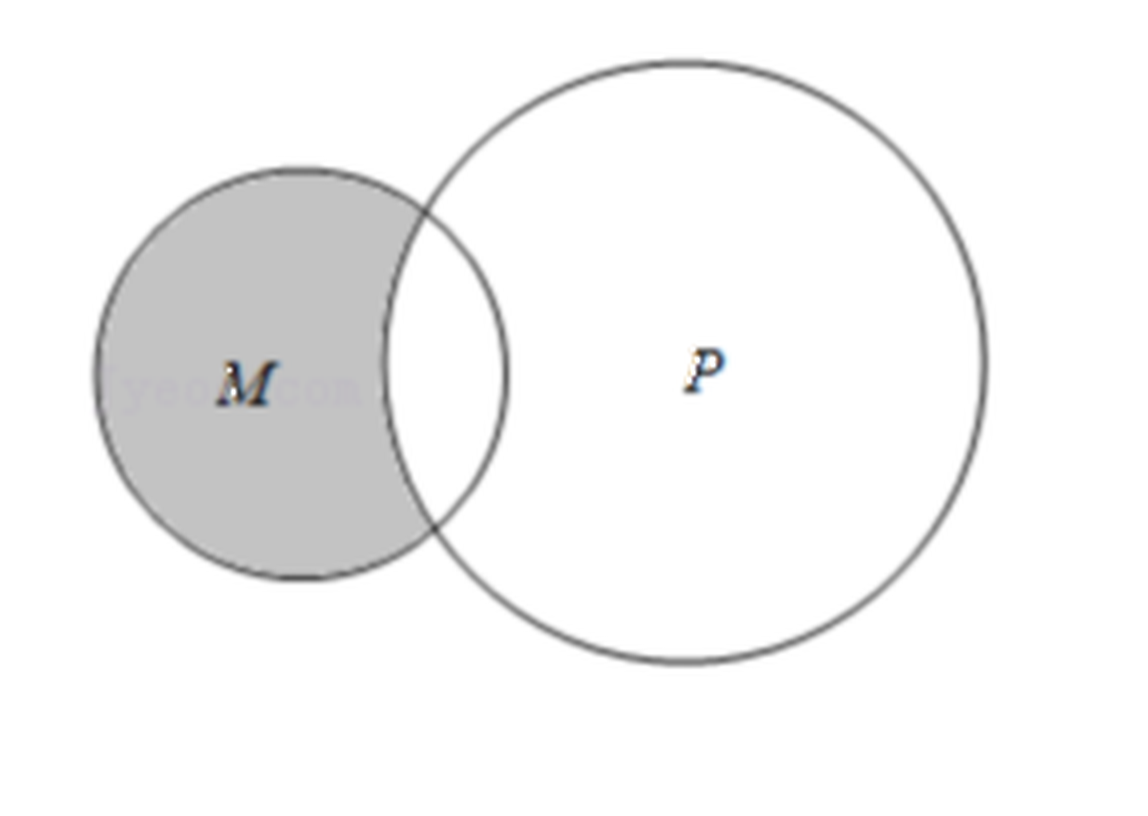
\includegraphics[width=0.36\textwidth]{figures/venn_M_shaded_P.png}
\end{center}

\step{阴影部分表示 $M-P$，所以 $M-(M-P)=M\cap P$. 故选 $B$.}
\solend

\fi

\item 设 $A_1$、$A_2$、$\cdots$、$A_7$ 均是含有 2 个元素的集合，且满足：

$A_i\cap A_{i+1}=\varnothing(i=1,2,3,4,5,6)$，$A_1\cap A_7=\varnothing$. 记 $B=A_1\cup A_2\cup\cdots\cup A_7$，则 $B$ 中元素个数的最小值是\mbox{（\quad）}

\keepwithprev
A. $4$\qquad B. $5$\qquad C. $6$\qquad D. $7$

\ans{$B$}

\ifanswer
\solbegin
\step{$A_1\cap A_7=\varnothing$，$A_i\cap A_{i+1}=\varnothing(i=1,2,3,4,5,6)$，}
\step{所以 $A_1$ 与 $A_2$ 的元素不同，则 $A_1\cup A_2$ 元素个数为 $4$，}
\step{若 $B$ 中元素个数的最小值是 $4$，则只能是 $A_3=A_1=A_5=A_7$，$A_4=A_2=A_6$，}
\step{与 $A_1\cap A_7=\varnothing$ 矛盾，}
\step{若 $A_3$ 从 $A_1$ 中选择 1 个元素，再加入一个新元素，}
\step{这样 $A_1\cup A_2\cup A_3$ 元素个数为 5 个，}
\step{这 5 个元素适当排列，得到 $A_4$、$A_5$、$A_6$、$A_7$，}
\step{例如 $A_1=\{1,2\},A_2=\{3,4\},A_3=\{1,5\}$，}
\step{取 $A_4=\{2,4\},A_5=\{3,5\},A_6=\{1,2\},A_7=\{3,5\}$，符合题意，}
\step{则 $B$ 中元素个数的最小值是 $2+2+1=5$，故选 $B$.}
\solend

\fi

\end{enumerate}

\bigsec{三、解答题}

\begin{enumerate}
\setcounter{enumi}{13}

\item 设 $A=\{x\mid x^2-ax+a^2-19=0\}$，$B=\{x\mid x^2-5x+6=0\}$，$C=\{x\mid x^2+2x-8=0\}$.

\begin{enumerate}[label=(\arabic*)]
\item 若 $A\cap B$ 非空，且 $A\cap C=\varnothing$，求 $a$ 的值；
\item $A\cap B=A\cap C\neq\varnothing$，求 $a$ 的值.
\end{enumerate}

\ifanswer
\solbegin
\stepm{(1)}{由题意，$C=\{-4,2\}$，}
\step{因为 $A\cap B$ 非空且 $A\cap C=\varnothing$，所以 $3\in A$，}
\step{即 $9-3a+a^2-19=0$，解得 $a=-2$ 或 $a=5$，}
\step{当 $a=-2$ 时，$A=\{3,-5\}$，满足题意；}
\step{当 $a=5$ 时，$A=\{2,3\}$，此时 $A\cap C=\{2\}$，不满足题意；}
\step{综上，$a=-2$；}
\stepm{(2)}{因为 $A\cap B=A\cap C\neq\varnothing$，所以 $2\in A$，}
\step{即 $4-2a+a^2-19=0$，解得 $a=-3$ 或 $a=5$，}
\step{当 $a=-3$ 时，$A=\{2,-5\}$，满足题意；}
\step{当 $a=5$ 时，$A=\{2,3\}$，不满足题意，}
\step{故 $a=-3$.}
\solend

\fi

\ansspace[6]

\item 已知 $A=\{x\mid x<-3\text{ 或 }x>1\}$.

\begin{enumerate}[label=(\arabic*)]
\item 若 $B=\{x\mid x<3m+1\text{ 或 }x>m+2\}$，$A\sub B$，求 $m$ 的取值范围.
\item 若 $B=\{x\mid m+2<x<3m+1\}$，$B\sub A$，求 $m$ 的取值范围.
\end{enumerate}

\ifanswer
\solbegin
\stepm{(1)}{当 $3m+1>m+2$，即 $m>\dfrac{1}{2}$ 时，$B=\R$，满足 $A\sub B$；}
\step{当 $3m+1\leqslant m+2$，即 $m\leqslant\dfrac{1}{2}$ 时，要使 $A\sub B$，}
\step{得 $\begin{cases}3m+1\geqslant-3\text{ ①}\\ m+2\leqslant 1\text{ ②}\end{cases}$，解得 $-\dfrac{4}{3}\leqslant m\leqslant-1$.}
\step{综上所述，$m$ 的取值范围为 $\left\{m\mid -\dfrac{4}{3}\leqslant m\leqslant-1\text{ 或 }m>\dfrac{1}{2}\right\}$；}
\stepm{(2)}{当 $B=\varnothing$ 时，则 $3m+1\leqslant m+2$，即 $m\leqslant\dfrac{1}{2}$ 时，满足 $B\sub A$；}
\step{当 $B\neq\varnothing$ 时，且 $B\sub A$，则 $\begin{cases}3m+1>m+2\\ 3m+1\leqslant-3\text{ 或 }m+2\geqslant 1\end{cases}$，所以 $m>\dfrac{1}{2}$.}
\step{综上所述，$m$ 的取值范围为 $\R$.}
\solend

\fi

\ansspace[6]

% 压轴题：其后已无内容，故作答区全用可丢弃胶水（\ansspace*），并在题目前先量一下版面。
\ansneed{7cm}

\item 已知集合 $A$ 为非空集合，定义

$S=\{x\mid x=a+b,a,b\in A\},T=\{x\mid x=|a-b|,a,b\in A\}$.

\begin{enumerate}[label=(\arabic*)]
\item 若集合 $A=\{1,3\}$，直接写出集合 $S$、$T$（无需写计算过程）；
\item 若集合 $A=\{x_1,x_2,x_3,x_4\}$，$x_1<x_2<x_3<x_4$，且 $T=A$，求证：$x_1+x_4=x_2+x_3$；
\item 若集合 $A=\{x\mid 0\leqslant x\leqslant 2021,x\in\N\}$，$S\cap T=\varnothing$. 记 $|A|$ 为集合 $A$ 中元素的个数，求 $|A|$ 的最大值.
\end{enumerate}

\ifanswer
\solbegin
\stepm{(1)}{$S=\{2,4,6\},T=\{0,2\}$；}
\stepm{(2)}{集合 $T$ 中最小的元素为 0，因为 $T=A$，且 $x_1<x_2<x_3<x_4$，所以 $x_1=0$，}
\step{所以集合 $T$ 中元素为 $x_2-x_1=x_2,x_3-x_1=x_3,x_4-x_1=x_4$，}
\step{以及 $x_3-x_2,x_4-x_2,x_4-x_3$ 均属于 $A$，}
% 注：本行原卷印「所以 $x_3$ 即 $x_4-x_2=x_3-x_1$」，「所以 $x_3$ 即 …」语义不完整，
%     疑有漏排（按本段结论应得 $x_4-x_2=x_3$），无法确证原意，本稿照抄原卷、未改。
\step{因为 $x_1=0<x_3-x_2<x_4-x_2<x_4$，所以 $x_3$ 即 $x_4-x_2=x_3-x_1$，}
\step{即 $x_1+x_4=x_2+x_3$；}
\stepm{(3)}{设 $A=\{a_1,a_2,a_3,\cdots,a_k\}$ 满足题意，其中 $a_1<a_2<\cdots<a_k$，}
\step{则 $2a_1<a_1+a_2<\cdots<a_1+a_k<a_2+a_k<a_3+a_k<\cdots<a_{k-1}+a_k<2a_k$，}
\step{所以 $|S\cup T|\leqslant 2k+1$，所以 $3k-1\leqslant 2a_k+1\leqslant 4043(k\in\N^*)$，}
\step{所以 $k\leqslant 1348$，}
\step{实际上当 $A=\{674,675,676,\cdots,2021\}$ 时满足题意，}
\step{证明如下：设 $A=\{m,m+1,m+2,\cdots,2021\},m\in\N$，}
\step{设 $S=\{2m,2m+1,2m+2,\cdots,4042\}$，$T=\{0,1,2,\cdots,2021-m\}$，}
\step{由题意得 $2021-m<2m$，即 $m>673\dfrac{2}{3}$，}
\step{故 $m$ 的最小值是 674，于是当 $m=674$，$A$ 中的元素最多，}
\step{即 $A=\{674,675,676,\cdots,2021\}$ 时满足题意，}
\step{综上所述，集合 $A$ 中元素的个数的最大值是 $1348$.}
\solend

\fi

\ansspace*[9]

\end{enumerate}

\bigsec{附加题}

\begin{enumerate}
\setcounter{enumi}{16}

\item 设 $A$ 是整数集的一个非空子集，对于 $k\in A$，如果 $k-1\notin A$ 且 $k+1\notin A$，那么 $k$ 是 $A$ 的一个“孤立元”。给定 $S=\{1,2,3,4,5,6,7,8\}$，由 $S$ 的 3 个元素构成的所有集合中，不含“孤立元”的集合共有 \blankline[2.4em] 个.

\ifanswer
\solbegin
\step{由题意得，“孤立元”即为在集合中无与之相邻的元素，}
\step{满足条件的集合有 $\{1,2,3\},\{2,3,4\},\{3,4,5\},\{4,5,6\},\{5,6,7\},\{6,7,8\}$，}
\step{共 6 个集合.}
\solend

\fi

\item 已知 $A\cap B=\varnothing$，$M=\{T\mid T\sub A\}$，$P=\{S\mid S\sub B\}$，则 $M\cap P=$ \blankline[4.4em].

\ans{$\{\varnothing\}$}

\item 已知集合 $A=\{x\mid x=m^2-n^2,m,n\in\Z\}$，写出所有满足集合 $A$ 的偶数 \blankline[4.4em].

\ans{$4n,n\in\Z$}

\item 对于给定的正整数 $n(n\geqslant 2)$ 若有限集合 $A=\{a_1,a_2,\cdots,a_n\}\sub M$，且满足

$a_1+a_2+\cdots+a_n=a_1\cdot a_2\cdots a_n$，则称 $A$ 为集合 $M$ 的 $n$ 元“调和子集”，则自然数集 $\N$ 的所有 3 元“调和子集”为 \blankline[3.6em].

\ans{$\{1,2,3\}$}

\end{enumerate}

\end{document}
"
% 紧凑版：xelatex "\def\iscompact{1}% 高一15_七宝中学_抱孩子练习.tex
%   —— 高一上数学「2026-2027 年七宝中学高一上抱孩子练习 9.8」（试卷版/答案版）
% 试卷版：xelatex 高一15_七宝中学_抱孩子练习.tex
% 答案版：xelatex "\def\isanswer{1}\input{高一15_七宝中学_抱孩子练习.tex}"
% 紧凑版：xelatex "\def\iscompact{1}\input{高一15_七宝中学_抱孩子练习.tex}"
%
% 原始材料是微信公众号图文（公众号「魔都数学加油站」），正文为 7 张 PNG 页（1080×1527）。
% 原文本身就是一份**讲评版**——题目下方直接印出【答案】或【解析】。试题文字、答案与解析
% 均照原卷录入，未改内容。卷面上的粉色斜水印「魔都数学加油站」属水印，未录入。
%
% 卷首标题：原卷印作「2026-2027 年七宝中学高一上抱孩子练习 9.8」——「抱孩子练习」四字
% 确系原卷所印（已放大 imgs_B/00.png 卷首核对），句末的「9.8」亦印在同一标题行内，
% 本稿一并照录，未改作「周末作业」；年份区间按全稿惯例排 en dash。
%
% 与原卷的排版差异（均已在 README「说明」中交代）：
%   ① 原文自**第 3 题**起（第 1、2 题未在该文中发布），故本稿题号亦自 3 起；
%   ② 原卷本就印有「一、填空题」「二、选择题」「三、解答题」三节标题，末节另印「附加题」，
%      本稿照原卷分节，只把标题改排成全稿统一的「大节标题」样式；
%   ③ 原卷填空、选择的答案直接印在题目下方，本稿统一改为试卷版隐去、答案版以【答案】或
%      【解析】给出（第 11 题原卷的答案是写在解析末句「故选 B」里的），使两版彻底分离；
%   ④ 原卷的集合符号 $R$、$Z$、$N$ 有正体与粗体两种写法（第 4 题的 $\mathbf{R}$、
%      第 16(3)、17、19、20 题的 $\mathbf{N}$、$\mathbf{Z}$ 为粗体，第 15 题解析的 $B=R$
%      为正体），本稿按全稿惯例统一写作 $\R$、$\Z$、$\N$；
%   ⑤ 原卷用**半角**括号（第 13 题「$\varnothing(i=1,2,3,4,5,6)$」、第 16(1)「(无需写计算过程)」、
%      第 16(2)「$A=\{x_1,x_2,x_3,x_4\}$」、第 20 题「$n(n\geqslant 2)$」），本稿按全稿惯例排全角；
%   ⑥ 原卷未印副标题，本稿按全稿惯例补出副标题「集合与常用逻辑用语」；
%   ⑦ 第 18、20 题的 $\subseteq$（带下划线，真包含写作 $\subset$ 与之形近）已逐处放大比对确认，
%      第 18 题的答案 $\{\varnothing\}$ 亦与 $\subseteq$ 口径相符（若为真包含则答案应为 $\varnothing$）。
%
% 原卷存疑两处（均已放大到能看清字形后核对，无法确证原意，本稿照抄原卷、未改）：
%   ① 第 10 题【解析】末句原卷印「所以 $1-k^2\neq 0$，即 $k\neq\pm 1$」——按此式，当 $k=1$
%      时两方程为同一直线、有无穷多解，$A\cap B\neq\varnothing$ 仍成立，故 $A\cap B\neq\varnothing$
%      当且仅当 $k\neq -1$；原卷结论与题设不合，疑为原卷笔误，但无法确证原意，本稿照抄原卷；
%   ② 第 16(2)【解析】原卷印「因为 $x_1=0<x_3-x_2<x_4-x_2<x_4$，所以 $x_3$ 即 $x_4-x_2=x_3-x_1$，」
%      ——「所以 $x_3$ 即 …」一句语义不完整，疑有漏排（按本段结论应得 $x_4-x_2=x_3$），
%      无法确证原意，本稿照抄原卷。

\documentclass[a4paper,11pt]{article}
\usepackage{common}

\begin{document}

\examtitlest[3]{2026--2027 年七宝中学高一上抱孩子练习 9.8}{集合与常用逻辑用语}

\bigsec{一、填空题}

\begin{enumerate}
\setcounter{enumi}{2}

\item 方程 $\sqrt{x+2}=-x$ 的解的集合为 \blankline[4.4em].

\ifanswer
\solbegin
\step{因为 $\sqrt{x+2}=-x$，所以 $\begin{cases}x\leqslant 0\\ x+2=x^2\end{cases}$，解得 $x=-1$，}
\step{所以方程 $\sqrt{x+2}=-x$ 的解的集合为 $\{-1\}$.}
\solend

\fi

\item 若 $A=\{x\mid a-4<x\leqslant a+4\}$，$B=\{x\mid x>5\text{ 或 }x<-1\}$，且 $A\cup B=\R$，则实数 $a$ 的取值范围是 \blankline[3.6em].

\ans{$[1,3)$}

\item 设集合 $A=\{x\mid x=2n+1,n\in\N\}$，$B=\{x\mid x=3n,n\in\N\}$，则 $A\cap B=$ \blankline[4.4em].

\ans{$\{x\mid x=6n+3,n\in\N\}$}

\item 已知集合 $A=\{1,2\}$，集合 $B=\{x\mid ax=6\}$，若 $A\cup B=A$，则 $a$ 的所有取值构成的集合为 \blankline[4.4em].

\ifanswer
\solbegin
\step{因为 $A\cup B=A$，所以 $B\sub A$，}
\step{当 $a=0$ 时，$B=\varnothing$，满足 $B\sub A$；}
\step{当 $a\neq 0$ 时，$B=\left\{\dfrac{6}{a}\right\}$，则 $\dfrac{6}{a}=1$ 或 $\dfrac{6}{a}=2$，解得 $a=6$ 或 $a=3$，}
\step{综上所述，$a$ 的所有取值构成的集合为 $\{0,3,6\}$.}
\solend

\fi

\item 设 $U=\{2,4,a^2-a+1\}$，$A=\{2,|a+1|\}$，$\overline{A}=\{7\}$，则 $a=$ \blankline[2.4em].

\ans{$3$}

\item 已知集合 $A=\{x\mid x^2-px-q=0\}$，$B=\{x\mid x^2+qx-p=0\}$，且 $A\cap B=\{1\}$，则 $A\cup B=$ \blankline[4.4em].

\ans{$\{0,-1,1\}$}

\item 定义集合运算：$A\odot B=\{z\mid z=xy(x+y),x\in A,y\in B\}$，若 $A=\{1,2\},B=\{3,4\}$，则 $A\odot B$ 的所有元素之和是 \blankline[3.6em].

\ans{$110$}

\item 已知集合 $A=\{(x,y)\mid kx+y=k+1\}$，$B=\{(x,y)\mid x+ky=2k\}$，其中 $k$ 为实数，$A\cap B\neq\varnothing$，则 $k$ 的取值范围是 \blankline[4.4em].

\ifanswer
\solbegin
\step{因为 $A\cap B\neq\varnothing$，所以方程组 $\begin{cases}kx+y=k+1\\ x+ky=2k\end{cases}$ 有解，消 $y$ 得 $(1-k^2)x=k-k^2$，}
% 注：末句原卷印「所以 $1-k^2\neq 0$，即 $k\neq\pm 1$」。按此式，$k=1$ 时两方程为同一直线、
%     有无穷多解，$A\cap B\neq\varnothing$ 仍成立，故结论应为 $k\neq -1$。疑为原卷笔误，
%     但无法确证原意，本稿照抄原卷、未改（详见文件头「原卷存疑」①）。
\step{所以 $1-k^2\neq 0$，即 $k\neq\pm 1$.}
\solend

\fi

\end{enumerate}

\bigsec{二、选择题}

\begin{enumerate}
\setcounter{enumi}{10}

\item 给出关系式：①$0\in\varnothing$；②$\varnothing=\{0\}$；③$\{a,b\}=\{b,a\}$；④$\{y\mid y=x^2-2\}=\{(x,y)\mid y=x^2-2\}$，其中正确的关系式的个数是\mbox{（\quad）}

\keepwithprev
A. $0$\qquad B. $1$\qquad C. $2$\qquad D. $3$

\ans{$B$}

\ifanswer
\solbegin
\step{在①中，$\varnothing$ 表示空集，$0\notin\varnothing$，故①错误；在②中，$\varnothing\sub\{0\}$，故②错误；}
\step{在③中，$\{a,b\}=\{b,a\}$，故③正确；}
\step{在④中，因为，$\{y\mid y=x^2-2\}$ 和 $\{(x,y)\mid y=x^2-2\}$ 的代表元素不同，}
\step{所以 $\{y\mid y=x^2-2\}\neq\{(x,y)\mid y=x^2-2\}$，故④错误.}
\step{故正确的是③，故选 $B$.}
\solend

\fi

\item 设集合 $M$、$P\neq\varnothing$，定义集合 $M-P=\{x\mid x\in M,x\notin P\}$，则集合 $M-(M-P)$ 是\mbox{（\quad）}

\keepwithprev
A. $P$\qquad B. $M$\qquad C. $M\cup P$\qquad D. $M\cap P$

\ans{$B$}

\ifanswer
\solbegin
\step{$M-(M-P)=\{x\mid x\in M,\text{ 且 }x\notin(M-P)\}$，}
\step{用 venn 图表示集合 $M$、$P$ 的关系如图：}

\begin{center}
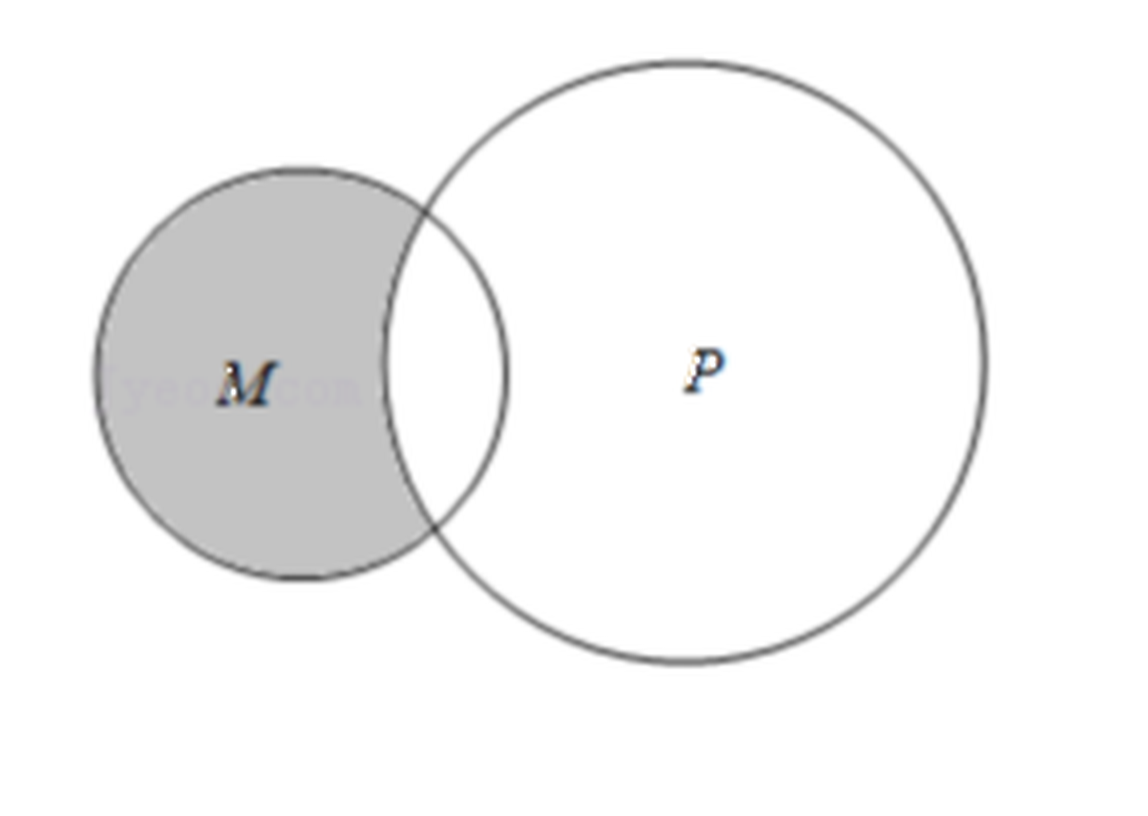
\includegraphics[width=0.36\textwidth]{figures/venn_M_shaded_P.png}
\end{center}

\step{阴影部分表示 $M-P$，所以 $M-(M-P)=M\cap P$. 故选 $B$.}
\solend

\fi

\item 设 $A_1$、$A_2$、$\cdots$、$A_7$ 均是含有 2 个元素的集合，且满足：

$A_i\cap A_{i+1}=\varnothing(i=1,2,3,4,5,6)$，$A_1\cap A_7=\varnothing$. 记 $B=A_1\cup A_2\cup\cdots\cup A_7$，则 $B$ 中元素个数的最小值是\mbox{（\quad）}

\keepwithprev
A. $4$\qquad B. $5$\qquad C. $6$\qquad D. $7$

\ans{$B$}

\ifanswer
\solbegin
\step{$A_1\cap A_7=\varnothing$，$A_i\cap A_{i+1}=\varnothing(i=1,2,3,4,5,6)$，}
\step{所以 $A_1$ 与 $A_2$ 的元素不同，则 $A_1\cup A_2$ 元素个数为 $4$，}
\step{若 $B$ 中元素个数的最小值是 $4$，则只能是 $A_3=A_1=A_5=A_7$，$A_4=A_2=A_6$，}
\step{与 $A_1\cap A_7=\varnothing$ 矛盾，}
\step{若 $A_3$ 从 $A_1$ 中选择 1 个元素，再加入一个新元素，}
\step{这样 $A_1\cup A_2\cup A_3$ 元素个数为 5 个，}
\step{这 5 个元素适当排列，得到 $A_4$、$A_5$、$A_6$、$A_7$，}
\step{例如 $A_1=\{1,2\},A_2=\{3,4\},A_3=\{1,5\}$，}
\step{取 $A_4=\{2,4\},A_5=\{3,5\},A_6=\{1,2\},A_7=\{3,5\}$，符合题意，}
\step{则 $B$ 中元素个数的最小值是 $2+2+1=5$，故选 $B$.}
\solend

\fi

\end{enumerate}

\bigsec{三、解答题}

\begin{enumerate}
\setcounter{enumi}{13}

\item 设 $A=\{x\mid x^2-ax+a^2-19=0\}$，$B=\{x\mid x^2-5x+6=0\}$，$C=\{x\mid x^2+2x-8=0\}$.

\begin{enumerate}[label=(\arabic*)]
\item 若 $A\cap B$ 非空，且 $A\cap C=\varnothing$，求 $a$ 的值；
\item $A\cap B=A\cap C\neq\varnothing$，求 $a$ 的值.
\end{enumerate}

\ifanswer
\solbegin
\stepm{(1)}{由题意，$C=\{-4,2\}$，}
\step{因为 $A\cap B$ 非空且 $A\cap C=\varnothing$，所以 $3\in A$，}
\step{即 $9-3a+a^2-19=0$，解得 $a=-2$ 或 $a=5$，}
\step{当 $a=-2$ 时，$A=\{3,-5\}$，满足题意；}
\step{当 $a=5$ 时，$A=\{2,3\}$，此时 $A\cap C=\{2\}$，不满足题意；}
\step{综上，$a=-2$；}
\stepm{(2)}{因为 $A\cap B=A\cap C\neq\varnothing$，所以 $2\in A$，}
\step{即 $4-2a+a^2-19=0$，解得 $a=-3$ 或 $a=5$，}
\step{当 $a=-3$ 时，$A=\{2,-5\}$，满足题意；}
\step{当 $a=5$ 时，$A=\{2,3\}$，不满足题意，}
\step{故 $a=-3$.}
\solend

\fi

\ansspace[6]

\item 已知 $A=\{x\mid x<-3\text{ 或 }x>1\}$.

\begin{enumerate}[label=(\arabic*)]
\item 若 $B=\{x\mid x<3m+1\text{ 或 }x>m+2\}$，$A\sub B$，求 $m$ 的取值范围.
\item 若 $B=\{x\mid m+2<x<3m+1\}$，$B\sub A$，求 $m$ 的取值范围.
\end{enumerate}

\ifanswer
\solbegin
\stepm{(1)}{当 $3m+1>m+2$，即 $m>\dfrac{1}{2}$ 时，$B=\R$，满足 $A\sub B$；}
\step{当 $3m+1\leqslant m+2$，即 $m\leqslant\dfrac{1}{2}$ 时，要使 $A\sub B$，}
\step{得 $\begin{cases}3m+1\geqslant-3\text{ ①}\\ m+2\leqslant 1\text{ ②}\end{cases}$，解得 $-\dfrac{4}{3}\leqslant m\leqslant-1$.}
\step{综上所述，$m$ 的取值范围为 $\left\{m\mid -\dfrac{4}{3}\leqslant m\leqslant-1\text{ 或 }m>\dfrac{1}{2}\right\}$；}
\stepm{(2)}{当 $B=\varnothing$ 时，则 $3m+1\leqslant m+2$，即 $m\leqslant\dfrac{1}{2}$ 时，满足 $B\sub A$；}
\step{当 $B\neq\varnothing$ 时，且 $B\sub A$，则 $\begin{cases}3m+1>m+2\\ 3m+1\leqslant-3\text{ 或 }m+2\geqslant 1\end{cases}$，所以 $m>\dfrac{1}{2}$.}
\step{综上所述，$m$ 的取值范围为 $\R$.}
\solend

\fi

\ansspace[6]

% 压轴题：其后已无内容，故作答区全用可丢弃胶水（\ansspace*），并在题目前先量一下版面。
\ansneed{7cm}

\item 已知集合 $A$ 为非空集合，定义

$S=\{x\mid x=a+b,a,b\in A\},T=\{x\mid x=|a-b|,a,b\in A\}$.

\begin{enumerate}[label=(\arabic*)]
\item 若集合 $A=\{1,3\}$，直接写出集合 $S$、$T$（无需写计算过程）；
\item 若集合 $A=\{x_1,x_2,x_3,x_4\}$，$x_1<x_2<x_3<x_4$，且 $T=A$，求证：$x_1+x_4=x_2+x_3$；
\item 若集合 $A=\{x\mid 0\leqslant x\leqslant 2021,x\in\N\}$，$S\cap T=\varnothing$. 记 $|A|$ 为集合 $A$ 中元素的个数，求 $|A|$ 的最大值.
\end{enumerate}

\ifanswer
\solbegin
\stepm{(1)}{$S=\{2,4,6\},T=\{0,2\}$；}
\stepm{(2)}{集合 $T$ 中最小的元素为 0，因为 $T=A$，且 $x_1<x_2<x_3<x_4$，所以 $x_1=0$，}
\step{所以集合 $T$ 中元素为 $x_2-x_1=x_2,x_3-x_1=x_3,x_4-x_1=x_4$，}
\step{以及 $x_3-x_2,x_4-x_2,x_4-x_3$ 均属于 $A$，}
% 注：本行原卷印「所以 $x_3$ 即 $x_4-x_2=x_3-x_1$」，「所以 $x_3$ 即 …」语义不完整，
%     疑有漏排（按本段结论应得 $x_4-x_2=x_3$），无法确证原意，本稿照抄原卷、未改。
\step{因为 $x_1=0<x_3-x_2<x_4-x_2<x_4$，所以 $x_3$ 即 $x_4-x_2=x_3-x_1$，}
\step{即 $x_1+x_4=x_2+x_3$；}
\stepm{(3)}{设 $A=\{a_1,a_2,a_3,\cdots,a_k\}$ 满足题意，其中 $a_1<a_2<\cdots<a_k$，}
\step{则 $2a_1<a_1+a_2<\cdots<a_1+a_k<a_2+a_k<a_3+a_k<\cdots<a_{k-1}+a_k<2a_k$，}
\step{所以 $|S\cup T|\leqslant 2k+1$，所以 $3k-1\leqslant 2a_k+1\leqslant 4043(k\in\N^*)$，}
\step{所以 $k\leqslant 1348$，}
\step{实际上当 $A=\{674,675,676,\cdots,2021\}$ 时满足题意，}
\step{证明如下：设 $A=\{m,m+1,m+2,\cdots,2021\},m\in\N$，}
\step{设 $S=\{2m,2m+1,2m+2,\cdots,4042\}$，$T=\{0,1,2,\cdots,2021-m\}$，}
\step{由题意得 $2021-m<2m$，即 $m>673\dfrac{2}{3}$，}
\step{故 $m$ 的最小值是 674，于是当 $m=674$，$A$ 中的元素最多，}
\step{即 $A=\{674,675,676,\cdots,2021\}$ 时满足题意，}
\step{综上所述，集合 $A$ 中元素的个数的最大值是 $1348$.}
\solend

\fi

\ansspace*[9]

\end{enumerate}

\bigsec{附加题}

\begin{enumerate}
\setcounter{enumi}{16}

\item 设 $A$ 是整数集的一个非空子集，对于 $k\in A$，如果 $k-1\notin A$ 且 $k+1\notin A$，那么 $k$ 是 $A$ 的一个“孤立元”。给定 $S=\{1,2,3,4,5,6,7,8\}$，由 $S$ 的 3 个元素构成的所有集合中，不含“孤立元”的集合共有 \blankline[2.4em] 个.

\ifanswer
\solbegin
\step{由题意得，“孤立元”即为在集合中无与之相邻的元素，}
\step{满足条件的集合有 $\{1,2,3\},\{2,3,4\},\{3,4,5\},\{4,5,6\},\{5,6,7\},\{6,7,8\}$，}
\step{共 6 个集合.}
\solend

\fi

\item 已知 $A\cap B=\varnothing$，$M=\{T\mid T\sub A\}$，$P=\{S\mid S\sub B\}$，则 $M\cap P=$ \blankline[4.4em].

\ans{$\{\varnothing\}$}

\item 已知集合 $A=\{x\mid x=m^2-n^2,m,n\in\Z\}$，写出所有满足集合 $A$ 的偶数 \blankline[4.4em].

\ans{$4n,n\in\Z$}

\item 对于给定的正整数 $n(n\geqslant 2)$ 若有限集合 $A=\{a_1,a_2,\cdots,a_n\}\sub M$，且满足

$a_1+a_2+\cdots+a_n=a_1\cdot a_2\cdots a_n$，则称 $A$ 为集合 $M$ 的 $n$ 元“调和子集”，则自然数集 $\N$ 的所有 3 元“调和子集”为 \blankline[3.6em].

\ans{$\{1,2,3\}$}

\end{enumerate}

\end{document}
"
%
% 原始材料是微信公众号图文（公众号「魔都数学加油站」），正文为 7 张 PNG 页（1080×1527）。
% 原文本身就是一份**讲评版**——题目下方直接印出【答案】或【解析】。试题文字、答案与解析
% 均照原卷录入，未改内容。卷面上的粉色斜水印「魔都数学加油站」属水印，未录入。
%
% 卷首标题：原卷印作「2026-2027 年七宝中学高一上抱孩子练习 9.8」——「抱孩子练习」四字
% 确系原卷所印（已放大 imgs_B/00.png 卷首核对），句末的「9.8」亦印在同一标题行内，
% 本稿一并照录，未改作「周末作业」；年份区间按全稿惯例排 en dash。
%
% 与原卷的排版差异（均已在 README「说明」中交代）：
%   ① 原文自**第 3 题**起（第 1、2 题未在该文中发布），故本稿题号亦自 3 起；
%   ② 原卷本就印有「一、填空题」「二、选择题」「三、解答题」三节标题，末节另印「附加题」，
%      本稿照原卷分节，只把标题改排成全稿统一的「大节标题」样式；
%   ③ 原卷填空、选择的答案直接印在题目下方，本稿统一改为试卷版隐去、答案版以【答案】或
%      【解析】给出（第 11 题原卷的答案是写在解析末句「故选 B」里的），使两版彻底分离；
%   ④ 原卷的集合符号 $R$、$Z$、$N$ 有正体与粗体两种写法（第 4 题的 $\mathbf{R}$、
%      第 16(3)、17、19、20 题的 $\mathbf{N}$、$\mathbf{Z}$ 为粗体，第 15 题解析的 $B=R$
%      为正体），本稿按全稿惯例统一写作 $\R$、$\Z$、$\N$；
%   ⑤ 原卷用**半角**括号（第 13 题「$\varnothing(i=1,2,3,4,5,6)$」、第 16(1)「(无需写计算过程)」、
%      第 16(2)「$A=\{x_1,x_2,x_3,x_4\}$」、第 20 题「$n(n\geqslant 2)$」），本稿按全稿惯例排全角；
%   ⑥ 原卷未印副标题，本稿按全稿惯例补出副标题「集合与常用逻辑用语」；
%   ⑦ 第 18、20 题的 $\subseteq$（带下划线，真包含写作 $\subset$ 与之形近）已逐处放大比对确认，
%      第 18 题的答案 $\{\varnothing\}$ 亦与 $\subseteq$ 口径相符（若为真包含则答案应为 $\varnothing$）。
%
% 原卷存疑两处（均已放大到能看清字形后核对，无法确证原意，本稿照抄原卷、未改）：
%   ① 第 10 题【解析】末句原卷印「所以 $1-k^2\neq 0$，即 $k\neq\pm 1$」——按此式，当 $k=1$
%      时两方程为同一直线、有无穷多解，$A\cap B\neq\varnothing$ 仍成立，故 $A\cap B\neq\varnothing$
%      当且仅当 $k\neq -1$；原卷结论与题设不合，疑为原卷笔误，但无法确证原意，本稿照抄原卷；
%   ② 第 16(2)【解析】原卷印「因为 $x_1=0<x_3-x_2<x_4-x_2<x_4$，所以 $x_3$ 即 $x_4-x_2=x_3-x_1$，」
%      ——「所以 $x_3$ 即 …」一句语义不完整，疑有漏排（按本段结论应得 $x_4-x_2=x_3$），
%      无法确证原意，本稿照抄原卷。

\documentclass[a4paper,11pt]{article}
\usepackage{common}

\begin{document}

\examtitlest[3]{2026--2027 年七宝中学高一上抱孩子练习 9.8}{集合与常用逻辑用语}

\bigsec{一、填空题}

\begin{enumerate}
\setcounter{enumi}{2}

\item 方程 $\sqrt{x+2}=-x$ 的解的集合为 \blankline[4.4em].

\ifanswer
\solbegin
\step{因为 $\sqrt{x+2}=-x$，所以 $\begin{cases}x\leqslant 0\\ x+2=x^2\end{cases}$，解得 $x=-1$，}
\step{所以方程 $\sqrt{x+2}=-x$ 的解的集合为 $\{-1\}$.}
\solend

\fi

\item 若 $A=\{x\mid a-4<x\leqslant a+4\}$，$B=\{x\mid x>5\text{ 或 }x<-1\}$，且 $A\cup B=\R$，则实数 $a$ 的取值范围是 \blankline[3.6em].

\ans{$[1,3)$}

\item 设集合 $A=\{x\mid x=2n+1,n\in\N\}$，$B=\{x\mid x=3n,n\in\N\}$，则 $A\cap B=$ \blankline[4.4em].

\ans{$\{x\mid x=6n+3,n\in\N\}$}

\item 已知集合 $A=\{1,2\}$，集合 $B=\{x\mid ax=6\}$，若 $A\cup B=A$，则 $a$ 的所有取值构成的集合为 \blankline[4.4em].

\ifanswer
\solbegin
\step{因为 $A\cup B=A$，所以 $B\sub A$，}
\step{当 $a=0$ 时，$B=\varnothing$，满足 $B\sub A$；}
\step{当 $a\neq 0$ 时，$B=\left\{\dfrac{6}{a}\right\}$，则 $\dfrac{6}{a}=1$ 或 $\dfrac{6}{a}=2$，解得 $a=6$ 或 $a=3$，}
\step{综上所述，$a$ 的所有取值构成的集合为 $\{0,3,6\}$.}
\solend

\fi

\item 设 $U=\{2,4,a^2-a+1\}$，$A=\{2,|a+1|\}$，$\overline{A}=\{7\}$，则 $a=$ \blankline[2.4em].

\ans{$3$}

\item 已知集合 $A=\{x\mid x^2-px-q=0\}$，$B=\{x\mid x^2+qx-p=0\}$，且 $A\cap B=\{1\}$，则 $A\cup B=$ \blankline[4.4em].

\ans{$\{0,-1,1\}$}

\item 定义集合运算：$A\odot B=\{z\mid z=xy(x+y),x\in A,y\in B\}$，若 $A=\{1,2\},B=\{3,4\}$，则 $A\odot B$ 的所有元素之和是 \blankline[3.6em].

\ans{$110$}

\item 已知集合 $A=\{(x,y)\mid kx+y=k+1\}$，$B=\{(x,y)\mid x+ky=2k\}$，其中 $k$ 为实数，$A\cap B\neq\varnothing$，则 $k$ 的取值范围是 \blankline[4.4em].

\ifanswer
\solbegin
\step{因为 $A\cap B\neq\varnothing$，所以方程组 $\begin{cases}kx+y=k+1\\ x+ky=2k\end{cases}$ 有解，消 $y$ 得 $(1-k^2)x=k-k^2$，}
% 注：末句原卷印「所以 $1-k^2\neq 0$，即 $k\neq\pm 1$」。按此式，$k=1$ 时两方程为同一直线、
%     有无穷多解，$A\cap B\neq\varnothing$ 仍成立，故结论应为 $k\neq -1$。疑为原卷笔误，
%     但无法确证原意，本稿照抄原卷、未改（详见文件头「原卷存疑」①）。
\step{所以 $1-k^2\neq 0$，即 $k\neq\pm 1$.}
\solend

\fi

\end{enumerate}

\bigsec{二、选择题}

\begin{enumerate}
\setcounter{enumi}{10}

\item 给出关系式：①$0\in\varnothing$；②$\varnothing=\{0\}$；③$\{a,b\}=\{b,a\}$；④$\{y\mid y=x^2-2\}=\{(x,y)\mid y=x^2-2\}$，其中正确的关系式的个数是\mbox{（\quad）}

\keepwithprev
A. $0$\qquad B. $1$\qquad C. $2$\qquad D. $3$

\ans{$B$}

\ifanswer
\solbegin
\step{在①中，$\varnothing$ 表示空集，$0\notin\varnothing$，故①错误；在②中，$\varnothing\sub\{0\}$，故②错误；}
\step{在③中，$\{a,b\}=\{b,a\}$，故③正确；}
\step{在④中，因为，$\{y\mid y=x^2-2\}$ 和 $\{(x,y)\mid y=x^2-2\}$ 的代表元素不同，}
\step{所以 $\{y\mid y=x^2-2\}\neq\{(x,y)\mid y=x^2-2\}$，故④错误.}
\step{故正确的是③，故选 $B$.}
\solend

\fi

\item 设集合 $M$、$P\neq\varnothing$，定义集合 $M-P=\{x\mid x\in M,x\notin P\}$，则集合 $M-(M-P)$ 是\mbox{（\quad）}

\keepwithprev
A. $P$\qquad B. $M$\qquad C. $M\cup P$\qquad D. $M\cap P$

\ans{$B$}

\ifanswer
\solbegin
\step{$M-(M-P)=\{x\mid x\in M,\text{ 且 }x\notin(M-P)\}$，}
\step{用 venn 图表示集合 $M$、$P$ 的关系如图：}

\begin{center}
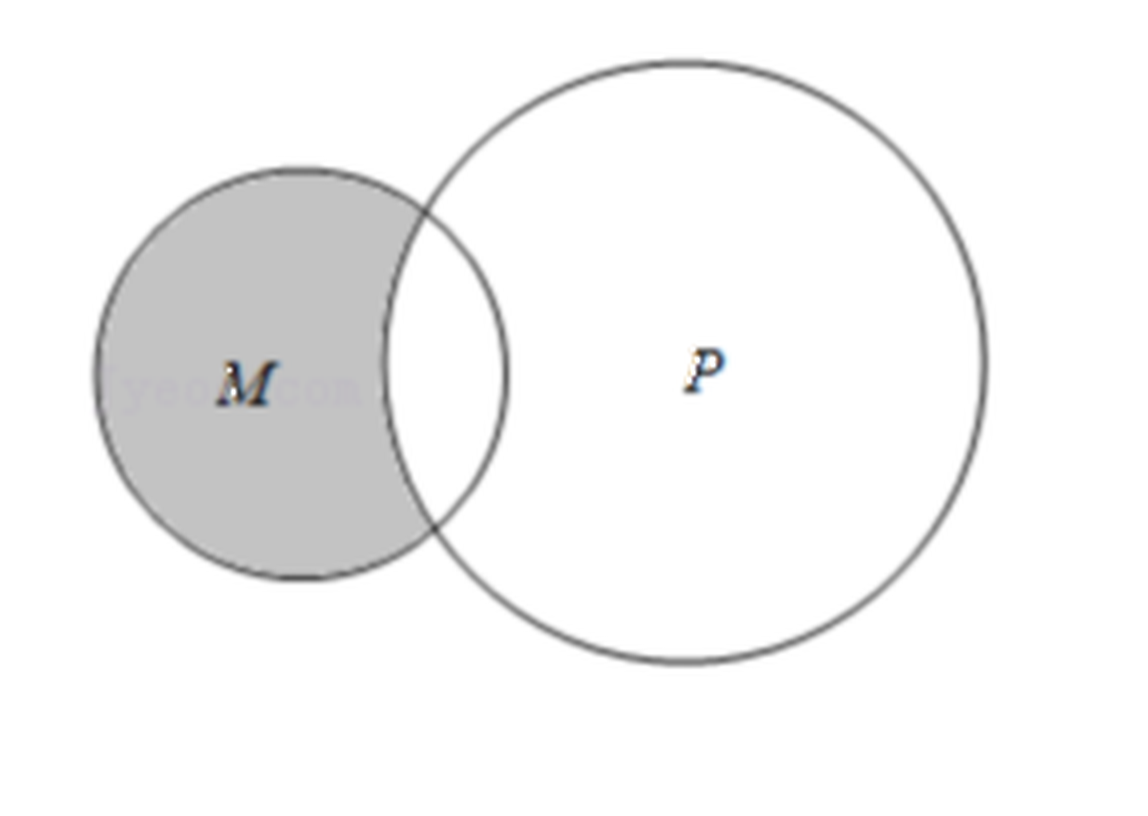
\includegraphics[width=0.36\textwidth]{figures/venn_M_shaded_P.png}
\end{center}

\step{阴影部分表示 $M-P$，所以 $M-(M-P)=M\cap P$. 故选 $B$.}
\solend

\fi

\item 设 $A_1$、$A_2$、$\cdots$、$A_7$ 均是含有 2 个元素的集合，且满足：

$A_i\cap A_{i+1}=\varnothing(i=1,2,3,4,5,6)$，$A_1\cap A_7=\varnothing$. 记 $B=A_1\cup A_2\cup\cdots\cup A_7$，则 $B$ 中元素个数的最小值是\mbox{（\quad）}

\keepwithprev
A. $4$\qquad B. $5$\qquad C. $6$\qquad D. $7$

\ans{$B$}

\ifanswer
\solbegin
\step{$A_1\cap A_7=\varnothing$，$A_i\cap A_{i+1}=\varnothing(i=1,2,3,4,5,6)$，}
\step{所以 $A_1$ 与 $A_2$ 的元素不同，则 $A_1\cup A_2$ 元素个数为 $4$，}
\step{若 $B$ 中元素个数的最小值是 $4$，则只能是 $A_3=A_1=A_5=A_7$，$A_4=A_2=A_6$，}
\step{与 $A_1\cap A_7=\varnothing$ 矛盾，}
\step{若 $A_3$ 从 $A_1$ 中选择 1 个元素，再加入一个新元素，}
\step{这样 $A_1\cup A_2\cup A_3$ 元素个数为 5 个，}
\step{这 5 个元素适当排列，得到 $A_4$、$A_5$、$A_6$、$A_7$，}
\step{例如 $A_1=\{1,2\},A_2=\{3,4\},A_3=\{1,5\}$，}
\step{取 $A_4=\{2,4\},A_5=\{3,5\},A_6=\{1,2\},A_7=\{3,5\}$，符合题意，}
\step{则 $B$ 中元素个数的最小值是 $2+2+1=5$，故选 $B$.}
\solend

\fi

\end{enumerate}

\bigsec{三、解答题}

\begin{enumerate}
\setcounter{enumi}{13}

\item 设 $A=\{x\mid x^2-ax+a^2-19=0\}$，$B=\{x\mid x^2-5x+6=0\}$，$C=\{x\mid x^2+2x-8=0\}$.

\begin{enumerate}[label=(\arabic*)]
\item 若 $A\cap B$ 非空，且 $A\cap C=\varnothing$，求 $a$ 的值；
\item $A\cap B=A\cap C\neq\varnothing$，求 $a$ 的值.
\end{enumerate}

\ifanswer
\solbegin
\stepm{(1)}{由题意，$C=\{-4,2\}$，}
\step{因为 $A\cap B$ 非空且 $A\cap C=\varnothing$，所以 $3\in A$，}
\step{即 $9-3a+a^2-19=0$，解得 $a=-2$ 或 $a=5$，}
\step{当 $a=-2$ 时，$A=\{3,-5\}$，满足题意；}
\step{当 $a=5$ 时，$A=\{2,3\}$，此时 $A\cap C=\{2\}$，不满足题意；}
\step{综上，$a=-2$；}
\stepm{(2)}{因为 $A\cap B=A\cap C\neq\varnothing$，所以 $2\in A$，}
\step{即 $4-2a+a^2-19=0$，解得 $a=-3$ 或 $a=5$，}
\step{当 $a=-3$ 时，$A=\{2,-5\}$，满足题意；}
\step{当 $a=5$ 时，$A=\{2,3\}$，不满足题意，}
\step{故 $a=-3$.}
\solend

\fi

\ansspace[6]

\item 已知 $A=\{x\mid x<-3\text{ 或 }x>1\}$.

\begin{enumerate}[label=(\arabic*)]
\item 若 $B=\{x\mid x<3m+1\text{ 或 }x>m+2\}$，$A\sub B$，求 $m$ 的取值范围.
\item 若 $B=\{x\mid m+2<x<3m+1\}$，$B\sub A$，求 $m$ 的取值范围.
\end{enumerate}

\ifanswer
\solbegin
\stepm{(1)}{当 $3m+1>m+2$，即 $m>\dfrac{1}{2}$ 时，$B=\R$，满足 $A\sub B$；}
\step{当 $3m+1\leqslant m+2$，即 $m\leqslant\dfrac{1}{2}$ 时，要使 $A\sub B$，}
\step{得 $\begin{cases}3m+1\geqslant-3\text{ ①}\\ m+2\leqslant 1\text{ ②}\end{cases}$，解得 $-\dfrac{4}{3}\leqslant m\leqslant-1$.}
\step{综上所述，$m$ 的取值范围为 $\left\{m\mid -\dfrac{4}{3}\leqslant m\leqslant-1\text{ 或 }m>\dfrac{1}{2}\right\}$；}
\stepm{(2)}{当 $B=\varnothing$ 时，则 $3m+1\leqslant m+2$，即 $m\leqslant\dfrac{1}{2}$ 时，满足 $B\sub A$；}
\step{当 $B\neq\varnothing$ 时，且 $B\sub A$，则 $\begin{cases}3m+1>m+2\\ 3m+1\leqslant-3\text{ 或 }m+2\geqslant 1\end{cases}$，所以 $m>\dfrac{1}{2}$.}
\step{综上所述，$m$ 的取值范围为 $\R$.}
\solend

\fi

\ansspace[6]

% 压轴题：其后已无内容，故作答区全用可丢弃胶水（\ansspace*），并在题目前先量一下版面。
\ansneed{7cm}

\item 已知集合 $A$ 为非空集合，定义

$S=\{x\mid x=a+b,a,b\in A\},T=\{x\mid x=|a-b|,a,b\in A\}$.

\begin{enumerate}[label=(\arabic*)]
\item 若集合 $A=\{1,3\}$，直接写出集合 $S$、$T$（无需写计算过程）；
\item 若集合 $A=\{x_1,x_2,x_3,x_4\}$，$x_1<x_2<x_3<x_4$，且 $T=A$，求证：$x_1+x_4=x_2+x_3$；
\item 若集合 $A=\{x\mid 0\leqslant x\leqslant 2021,x\in\N\}$，$S\cap T=\varnothing$. 记 $|A|$ 为集合 $A$ 中元素的个数，求 $|A|$ 的最大值.
\end{enumerate}

\ifanswer
\solbegin
\stepm{(1)}{$S=\{2,4,6\},T=\{0,2\}$；}
\stepm{(2)}{集合 $T$ 中最小的元素为 0，因为 $T=A$，且 $x_1<x_2<x_3<x_4$，所以 $x_1=0$，}
\step{所以集合 $T$ 中元素为 $x_2-x_1=x_2,x_3-x_1=x_3,x_4-x_1=x_4$，}
\step{以及 $x_3-x_2,x_4-x_2,x_4-x_3$ 均属于 $A$，}
% 注：本行原卷印「所以 $x_3$ 即 $x_4-x_2=x_3-x_1$」，「所以 $x_3$ 即 …」语义不完整，
%     疑有漏排（按本段结论应得 $x_4-x_2=x_3$），无法确证原意，本稿照抄原卷、未改。
\step{因为 $x_1=0<x_3-x_2<x_4-x_2<x_4$，所以 $x_3$ 即 $x_4-x_2=x_3-x_1$，}
\step{即 $x_1+x_4=x_2+x_3$；}
\stepm{(3)}{设 $A=\{a_1,a_2,a_3,\cdots,a_k\}$ 满足题意，其中 $a_1<a_2<\cdots<a_k$，}
\step{则 $2a_1<a_1+a_2<\cdots<a_1+a_k<a_2+a_k<a_3+a_k<\cdots<a_{k-1}+a_k<2a_k$，}
\step{所以 $|S\cup T|\leqslant 2k+1$，所以 $3k-1\leqslant 2a_k+1\leqslant 4043(k\in\N^*)$，}
\step{所以 $k\leqslant 1348$，}
\step{实际上当 $A=\{674,675,676,\cdots,2021\}$ 时满足题意，}
\step{证明如下：设 $A=\{m,m+1,m+2,\cdots,2021\},m\in\N$，}
\step{设 $S=\{2m,2m+1,2m+2,\cdots,4042\}$，$T=\{0,1,2,\cdots,2021-m\}$，}
\step{由题意得 $2021-m<2m$，即 $m>673\dfrac{2}{3}$，}
\step{故 $m$ 的最小值是 674，于是当 $m=674$，$A$ 中的元素最多，}
\step{即 $A=\{674,675,676,\cdots,2021\}$ 时满足题意，}
\step{综上所述，集合 $A$ 中元素的个数的最大值是 $1348$.}
\solend

\fi

\ansspace*[9]

\end{enumerate}

\bigsec{附加题}

\begin{enumerate}
\setcounter{enumi}{16}

\item 设 $A$ 是整数集的一个非空子集，对于 $k\in A$，如果 $k-1\notin A$ 且 $k+1\notin A$，那么 $k$ 是 $A$ 的一个“孤立元”。给定 $S=\{1,2,3,4,5,6,7,8\}$，由 $S$ 的 3 个元素构成的所有集合中，不含“孤立元”的集合共有 \blankline[2.4em] 个.

\ifanswer
\solbegin
\step{由题意得，“孤立元”即为在集合中无与之相邻的元素，}
\step{满足条件的集合有 $\{1,2,3\},\{2,3,4\},\{3,4,5\},\{4,5,6\},\{5,6,7\},\{6,7,8\}$，}
\step{共 6 个集合.}
\solend

\fi

\item 已知 $A\cap B=\varnothing$，$M=\{T\mid T\sub A\}$，$P=\{S\mid S\sub B\}$，则 $M\cap P=$ \blankline[4.4em].

\ans{$\{\varnothing\}$}

\item 已知集合 $A=\{x\mid x=m^2-n^2,m,n\in\Z\}$，写出所有满足集合 $A$ 的偶数 \blankline[4.4em].

\ans{$4n,n\in\Z$}

\item 对于给定的正整数 $n(n\geqslant 2)$ 若有限集合 $A=\{a_1,a_2,\cdots,a_n\}\sub M$，且满足

$a_1+a_2+\cdots+a_n=a_1\cdot a_2\cdots a_n$，则称 $A$ 为集合 $M$ 的 $n$ 元“调和子集”，则自然数集 $\N$ 的所有 3 元“调和子集”为 \blankline[3.6em].

\ans{$\{1,2,3\}$}

\end{enumerate}

\end{document}
"
% 紧凑版：xelatex "\def\iscompact{1}% 高一15_七宝中学_抱孩子练习.tex
%   —— 高一上数学「2026-2027 年七宝中学高一上抱孩子练习 9.8」（试卷版/答案版）
% 试卷版：xelatex 高一15_七宝中学_抱孩子练习.tex
% 答案版：xelatex "\def\isanswer{1}% 高一15_七宝中学_抱孩子练习.tex
%   —— 高一上数学「2026-2027 年七宝中学高一上抱孩子练习 9.8」（试卷版/答案版）
% 试卷版：xelatex 高一15_七宝中学_抱孩子练习.tex
% 答案版：xelatex "\def\isanswer{1}\input{高一15_七宝中学_抱孩子练习.tex}"
% 紧凑版：xelatex "\def\iscompact{1}\input{高一15_七宝中学_抱孩子练习.tex}"
%
% 原始材料是微信公众号图文（公众号「魔都数学加油站」），正文为 7 张 PNG 页（1080×1527）。
% 原文本身就是一份**讲评版**——题目下方直接印出【答案】或【解析】。试题文字、答案与解析
% 均照原卷录入，未改内容。卷面上的粉色斜水印「魔都数学加油站」属水印，未录入。
%
% 卷首标题：原卷印作「2026-2027 年七宝中学高一上抱孩子练习 9.8」——「抱孩子练习」四字
% 确系原卷所印（已放大 imgs_B/00.png 卷首核对），句末的「9.8」亦印在同一标题行内，
% 本稿一并照录，未改作「周末作业」；年份区间按全稿惯例排 en dash。
%
% 与原卷的排版差异（均已在 README「说明」中交代）：
%   ① 原文自**第 3 题**起（第 1、2 题未在该文中发布），故本稿题号亦自 3 起；
%   ② 原卷本就印有「一、填空题」「二、选择题」「三、解答题」三节标题，末节另印「附加题」，
%      本稿照原卷分节，只把标题改排成全稿统一的「大节标题」样式；
%   ③ 原卷填空、选择的答案直接印在题目下方，本稿统一改为试卷版隐去、答案版以【答案】或
%      【解析】给出（第 11 题原卷的答案是写在解析末句「故选 B」里的），使两版彻底分离；
%   ④ 原卷的集合符号 $R$、$Z$、$N$ 有正体与粗体两种写法（第 4 题的 $\mathbf{R}$、
%      第 16(3)、17、19、20 题的 $\mathbf{N}$、$\mathbf{Z}$ 为粗体，第 15 题解析的 $B=R$
%      为正体），本稿按全稿惯例统一写作 $\R$、$\Z$、$\N$；
%   ⑤ 原卷用**半角**括号（第 13 题「$\varnothing(i=1,2,3,4,5,6)$」、第 16(1)「(无需写计算过程)」、
%      第 16(2)「$A=\{x_1,x_2,x_3,x_4\}$」、第 20 题「$n(n\geqslant 2)$」），本稿按全稿惯例排全角；
%   ⑥ 原卷未印副标题，本稿按全稿惯例补出副标题「集合与常用逻辑用语」；
%   ⑦ 第 18、20 题的 $\subseteq$（带下划线，真包含写作 $\subset$ 与之形近）已逐处放大比对确认，
%      第 18 题的答案 $\{\varnothing\}$ 亦与 $\subseteq$ 口径相符（若为真包含则答案应为 $\varnothing$）。
%
% 原卷存疑两处（均已放大到能看清字形后核对，无法确证原意，本稿照抄原卷、未改）：
%   ① 第 10 题【解析】末句原卷印「所以 $1-k^2\neq 0$，即 $k\neq\pm 1$」——按此式，当 $k=1$
%      时两方程为同一直线、有无穷多解，$A\cap B\neq\varnothing$ 仍成立，故 $A\cap B\neq\varnothing$
%      当且仅当 $k\neq -1$；原卷结论与题设不合，疑为原卷笔误，但无法确证原意，本稿照抄原卷；
%   ② 第 16(2)【解析】原卷印「因为 $x_1=0<x_3-x_2<x_4-x_2<x_4$，所以 $x_3$ 即 $x_4-x_2=x_3-x_1$，」
%      ——「所以 $x_3$ 即 …」一句语义不完整，疑有漏排（按本段结论应得 $x_4-x_2=x_3$），
%      无法确证原意，本稿照抄原卷。

\documentclass[a4paper,11pt]{article}
\usepackage{common}

\begin{document}

\examtitlest[3]{2026--2027 年七宝中学高一上抱孩子练习 9.8}{集合与常用逻辑用语}

\bigsec{一、填空题}

\begin{enumerate}
\setcounter{enumi}{2}

\item 方程 $\sqrt{x+2}=-x$ 的解的集合为 \blankline[4.4em].

\ifanswer
\solbegin
\step{因为 $\sqrt{x+2}=-x$，所以 $\begin{cases}x\leqslant 0\\ x+2=x^2\end{cases}$，解得 $x=-1$，}
\step{所以方程 $\sqrt{x+2}=-x$ 的解的集合为 $\{-1\}$.}
\solend

\fi

\item 若 $A=\{x\mid a-4<x\leqslant a+4\}$，$B=\{x\mid x>5\text{ 或 }x<-1\}$，且 $A\cup B=\R$，则实数 $a$ 的取值范围是 \blankline[3.6em].

\ans{$[1,3)$}

\item 设集合 $A=\{x\mid x=2n+1,n\in\N\}$，$B=\{x\mid x=3n,n\in\N\}$，则 $A\cap B=$ \blankline[4.4em].

\ans{$\{x\mid x=6n+3,n\in\N\}$}

\item 已知集合 $A=\{1,2\}$，集合 $B=\{x\mid ax=6\}$，若 $A\cup B=A$，则 $a$ 的所有取值构成的集合为 \blankline[4.4em].

\ifanswer
\solbegin
\step{因为 $A\cup B=A$，所以 $B\sub A$，}
\step{当 $a=0$ 时，$B=\varnothing$，满足 $B\sub A$；}
\step{当 $a\neq 0$ 时，$B=\left\{\dfrac{6}{a}\right\}$，则 $\dfrac{6}{a}=1$ 或 $\dfrac{6}{a}=2$，解得 $a=6$ 或 $a=3$，}
\step{综上所述，$a$ 的所有取值构成的集合为 $\{0,3,6\}$.}
\solend

\fi

\item 设 $U=\{2,4,a^2-a+1\}$，$A=\{2,|a+1|\}$，$\overline{A}=\{7\}$，则 $a=$ \blankline[2.4em].

\ans{$3$}

\item 已知集合 $A=\{x\mid x^2-px-q=0\}$，$B=\{x\mid x^2+qx-p=0\}$，且 $A\cap B=\{1\}$，则 $A\cup B=$ \blankline[4.4em].

\ans{$\{0,-1,1\}$}

\item 定义集合运算：$A\odot B=\{z\mid z=xy(x+y),x\in A,y\in B\}$，若 $A=\{1,2\},B=\{3,4\}$，则 $A\odot B$ 的所有元素之和是 \blankline[3.6em].

\ans{$110$}

\item 已知集合 $A=\{(x,y)\mid kx+y=k+1\}$，$B=\{(x,y)\mid x+ky=2k\}$，其中 $k$ 为实数，$A\cap B\neq\varnothing$，则 $k$ 的取值范围是 \blankline[4.4em].

\ifanswer
\solbegin
\step{因为 $A\cap B\neq\varnothing$，所以方程组 $\begin{cases}kx+y=k+1\\ x+ky=2k\end{cases}$ 有解，消 $y$ 得 $(1-k^2)x=k-k^2$，}
% 注：末句原卷印「所以 $1-k^2\neq 0$，即 $k\neq\pm 1$」。按此式，$k=1$ 时两方程为同一直线、
%     有无穷多解，$A\cap B\neq\varnothing$ 仍成立，故结论应为 $k\neq -1$。疑为原卷笔误，
%     但无法确证原意，本稿照抄原卷、未改（详见文件头「原卷存疑」①）。
\step{所以 $1-k^2\neq 0$，即 $k\neq\pm 1$.}
\solend

\fi

\end{enumerate}

\bigsec{二、选择题}

\begin{enumerate}
\setcounter{enumi}{10}

\item 给出关系式：①$0\in\varnothing$；②$\varnothing=\{0\}$；③$\{a,b\}=\{b,a\}$；④$\{y\mid y=x^2-2\}=\{(x,y)\mid y=x^2-2\}$，其中正确的关系式的个数是\mbox{（\quad）}

\keepwithprev
A. $0$\qquad B. $1$\qquad C. $2$\qquad D. $3$

\ans{$B$}

\ifanswer
\solbegin
\step{在①中，$\varnothing$ 表示空集，$0\notin\varnothing$，故①错误；在②中，$\varnothing\sub\{0\}$，故②错误；}
\step{在③中，$\{a,b\}=\{b,a\}$，故③正确；}
\step{在④中，因为，$\{y\mid y=x^2-2\}$ 和 $\{(x,y)\mid y=x^2-2\}$ 的代表元素不同，}
\step{所以 $\{y\mid y=x^2-2\}\neq\{(x,y)\mid y=x^2-2\}$，故④错误.}
\step{故正确的是③，故选 $B$.}
\solend

\fi

\item 设集合 $M$、$P\neq\varnothing$，定义集合 $M-P=\{x\mid x\in M,x\notin P\}$，则集合 $M-(M-P)$ 是\mbox{（\quad）}

\keepwithprev
A. $P$\qquad B. $M$\qquad C. $M\cup P$\qquad D. $M\cap P$

\ans{$B$}

\ifanswer
\solbegin
\step{$M-(M-P)=\{x\mid x\in M,\text{ 且 }x\notin(M-P)\}$，}
\step{用 venn 图表示集合 $M$、$P$ 的关系如图：}

\begin{center}
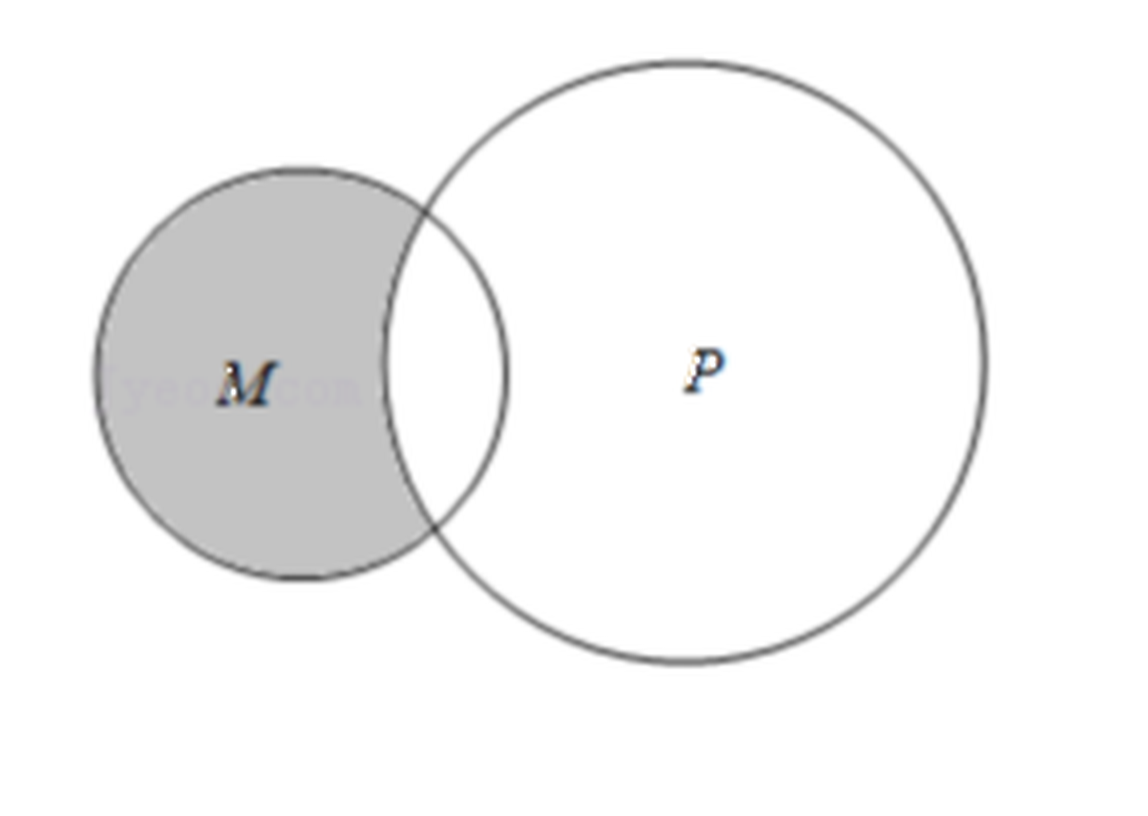
\includegraphics[width=0.36\textwidth]{figures/venn_M_shaded_P.png}
\end{center}

\step{阴影部分表示 $M-P$，所以 $M-(M-P)=M\cap P$. 故选 $B$.}
\solend

\fi

\item 设 $A_1$、$A_2$、$\cdots$、$A_7$ 均是含有 2 个元素的集合，且满足：

$A_i\cap A_{i+1}=\varnothing(i=1,2,3,4,5,6)$，$A_1\cap A_7=\varnothing$. 记 $B=A_1\cup A_2\cup\cdots\cup A_7$，则 $B$ 中元素个数的最小值是\mbox{（\quad）}

\keepwithprev
A. $4$\qquad B. $5$\qquad C. $6$\qquad D. $7$

\ans{$B$}

\ifanswer
\solbegin
\step{$A_1\cap A_7=\varnothing$，$A_i\cap A_{i+1}=\varnothing(i=1,2,3,4,5,6)$，}
\step{所以 $A_1$ 与 $A_2$ 的元素不同，则 $A_1\cup A_2$ 元素个数为 $4$，}
\step{若 $B$ 中元素个数的最小值是 $4$，则只能是 $A_3=A_1=A_5=A_7$，$A_4=A_2=A_6$，}
\step{与 $A_1\cap A_7=\varnothing$ 矛盾，}
\step{若 $A_3$ 从 $A_1$ 中选择 1 个元素，再加入一个新元素，}
\step{这样 $A_1\cup A_2\cup A_3$ 元素个数为 5 个，}
\step{这 5 个元素适当排列，得到 $A_4$、$A_5$、$A_6$、$A_7$，}
\step{例如 $A_1=\{1,2\},A_2=\{3,4\},A_3=\{1,5\}$，}
\step{取 $A_4=\{2,4\},A_5=\{3,5\},A_6=\{1,2\},A_7=\{3,5\}$，符合题意，}
\step{则 $B$ 中元素个数的最小值是 $2+2+1=5$，故选 $B$.}
\solend

\fi

\end{enumerate}

\bigsec{三、解答题}

\begin{enumerate}
\setcounter{enumi}{13}

\item 设 $A=\{x\mid x^2-ax+a^2-19=0\}$，$B=\{x\mid x^2-5x+6=0\}$，$C=\{x\mid x^2+2x-8=0\}$.

\begin{enumerate}[label=(\arabic*)]
\item 若 $A\cap B$ 非空，且 $A\cap C=\varnothing$，求 $a$ 的值；
\item $A\cap B=A\cap C\neq\varnothing$，求 $a$ 的值.
\end{enumerate}

\ifanswer
\solbegin
\stepm{(1)}{由题意，$C=\{-4,2\}$，}
\step{因为 $A\cap B$ 非空且 $A\cap C=\varnothing$，所以 $3\in A$，}
\step{即 $9-3a+a^2-19=0$，解得 $a=-2$ 或 $a=5$，}
\step{当 $a=-2$ 时，$A=\{3,-5\}$，满足题意；}
\step{当 $a=5$ 时，$A=\{2,3\}$，此时 $A\cap C=\{2\}$，不满足题意；}
\step{综上，$a=-2$；}
\stepm{(2)}{因为 $A\cap B=A\cap C\neq\varnothing$，所以 $2\in A$，}
\step{即 $4-2a+a^2-19=0$，解得 $a=-3$ 或 $a=5$，}
\step{当 $a=-3$ 时，$A=\{2,-5\}$，满足题意；}
\step{当 $a=5$ 时，$A=\{2,3\}$，不满足题意，}
\step{故 $a=-3$.}
\solend

\fi

\ansspace[6]

\item 已知 $A=\{x\mid x<-3\text{ 或 }x>1\}$.

\begin{enumerate}[label=(\arabic*)]
\item 若 $B=\{x\mid x<3m+1\text{ 或 }x>m+2\}$，$A\sub B$，求 $m$ 的取值范围.
\item 若 $B=\{x\mid m+2<x<3m+1\}$，$B\sub A$，求 $m$ 的取值范围.
\end{enumerate}

\ifanswer
\solbegin
\stepm{(1)}{当 $3m+1>m+2$，即 $m>\dfrac{1}{2}$ 时，$B=\R$，满足 $A\sub B$；}
\step{当 $3m+1\leqslant m+2$，即 $m\leqslant\dfrac{1}{2}$ 时，要使 $A\sub B$，}
\step{得 $\begin{cases}3m+1\geqslant-3\text{ ①}\\ m+2\leqslant 1\text{ ②}\end{cases}$，解得 $-\dfrac{4}{3}\leqslant m\leqslant-1$.}
\step{综上所述，$m$ 的取值范围为 $\left\{m\mid -\dfrac{4}{3}\leqslant m\leqslant-1\text{ 或 }m>\dfrac{1}{2}\right\}$；}
\stepm{(2)}{当 $B=\varnothing$ 时，则 $3m+1\leqslant m+2$，即 $m\leqslant\dfrac{1}{2}$ 时，满足 $B\sub A$；}
\step{当 $B\neq\varnothing$ 时，且 $B\sub A$，则 $\begin{cases}3m+1>m+2\\ 3m+1\leqslant-3\text{ 或 }m+2\geqslant 1\end{cases}$，所以 $m>\dfrac{1}{2}$.}
\step{综上所述，$m$ 的取值范围为 $\R$.}
\solend

\fi

\ansspace[6]

% 压轴题：其后已无内容，故作答区全用可丢弃胶水（\ansspace*），并在题目前先量一下版面。
\ansneed{7cm}

\item 已知集合 $A$ 为非空集合，定义

$S=\{x\mid x=a+b,a,b\in A\},T=\{x\mid x=|a-b|,a,b\in A\}$.

\begin{enumerate}[label=(\arabic*)]
\item 若集合 $A=\{1,3\}$，直接写出集合 $S$、$T$（无需写计算过程）；
\item 若集合 $A=\{x_1,x_2,x_3,x_4\}$，$x_1<x_2<x_3<x_4$，且 $T=A$，求证：$x_1+x_4=x_2+x_3$；
\item 若集合 $A=\{x\mid 0\leqslant x\leqslant 2021,x\in\N\}$，$S\cap T=\varnothing$. 记 $|A|$ 为集合 $A$ 中元素的个数，求 $|A|$ 的最大值.
\end{enumerate}

\ifanswer
\solbegin
\stepm{(1)}{$S=\{2,4,6\},T=\{0,2\}$；}
\stepm{(2)}{集合 $T$ 中最小的元素为 0，因为 $T=A$，且 $x_1<x_2<x_3<x_4$，所以 $x_1=0$，}
\step{所以集合 $T$ 中元素为 $x_2-x_1=x_2,x_3-x_1=x_3,x_4-x_1=x_4$，}
\step{以及 $x_3-x_2,x_4-x_2,x_4-x_3$ 均属于 $A$，}
% 注：本行原卷印「所以 $x_3$ 即 $x_4-x_2=x_3-x_1$」，「所以 $x_3$ 即 …」语义不完整，
%     疑有漏排（按本段结论应得 $x_4-x_2=x_3$），无法确证原意，本稿照抄原卷、未改。
\step{因为 $x_1=0<x_3-x_2<x_4-x_2<x_4$，所以 $x_3$ 即 $x_4-x_2=x_3-x_1$，}
\step{即 $x_1+x_4=x_2+x_3$；}
\stepm{(3)}{设 $A=\{a_1,a_2,a_3,\cdots,a_k\}$ 满足题意，其中 $a_1<a_2<\cdots<a_k$，}
\step{则 $2a_1<a_1+a_2<\cdots<a_1+a_k<a_2+a_k<a_3+a_k<\cdots<a_{k-1}+a_k<2a_k$，}
\step{所以 $|S\cup T|\leqslant 2k+1$，所以 $3k-1\leqslant 2a_k+1\leqslant 4043(k\in\N^*)$，}
\step{所以 $k\leqslant 1348$，}
\step{实际上当 $A=\{674,675,676,\cdots,2021\}$ 时满足题意，}
\step{证明如下：设 $A=\{m,m+1,m+2,\cdots,2021\},m\in\N$，}
\step{设 $S=\{2m,2m+1,2m+2,\cdots,4042\}$，$T=\{0,1,2,\cdots,2021-m\}$，}
\step{由题意得 $2021-m<2m$，即 $m>673\dfrac{2}{3}$，}
\step{故 $m$ 的最小值是 674，于是当 $m=674$，$A$ 中的元素最多，}
\step{即 $A=\{674,675,676,\cdots,2021\}$ 时满足题意，}
\step{综上所述，集合 $A$ 中元素的个数的最大值是 $1348$.}
\solend

\fi

\ansspace*[9]

\end{enumerate}

\bigsec{附加题}

\begin{enumerate}
\setcounter{enumi}{16}

\item 设 $A$ 是整数集的一个非空子集，对于 $k\in A$，如果 $k-1\notin A$ 且 $k+1\notin A$，那么 $k$ 是 $A$ 的一个“孤立元”。给定 $S=\{1,2,3,4,5,6,7,8\}$，由 $S$ 的 3 个元素构成的所有集合中，不含“孤立元”的集合共有 \blankline[2.4em] 个.

\ifanswer
\solbegin
\step{由题意得，“孤立元”即为在集合中无与之相邻的元素，}
\step{满足条件的集合有 $\{1,2,3\},\{2,3,4\},\{3,4,5\},\{4,5,6\},\{5,6,7\},\{6,7,8\}$，}
\step{共 6 个集合.}
\solend

\fi

\item 已知 $A\cap B=\varnothing$，$M=\{T\mid T\sub A\}$，$P=\{S\mid S\sub B\}$，则 $M\cap P=$ \blankline[4.4em].

\ans{$\{\varnothing\}$}

\item 已知集合 $A=\{x\mid x=m^2-n^2,m,n\in\Z\}$，写出所有满足集合 $A$ 的偶数 \blankline[4.4em].

\ans{$4n,n\in\Z$}

\item 对于给定的正整数 $n(n\geqslant 2)$ 若有限集合 $A=\{a_1,a_2,\cdots,a_n\}\sub M$，且满足

$a_1+a_2+\cdots+a_n=a_1\cdot a_2\cdots a_n$，则称 $A$ 为集合 $M$ 的 $n$ 元“调和子集”，则自然数集 $\N$ 的所有 3 元“调和子集”为 \blankline[3.6em].

\ans{$\{1,2,3\}$}

\end{enumerate}

\end{document}
"
% 紧凑版：xelatex "\def\iscompact{1}% 高一15_七宝中学_抱孩子练习.tex
%   —— 高一上数学「2026-2027 年七宝中学高一上抱孩子练习 9.8」（试卷版/答案版）
% 试卷版：xelatex 高一15_七宝中学_抱孩子练习.tex
% 答案版：xelatex "\def\isanswer{1}\input{高一15_七宝中学_抱孩子练习.tex}"
% 紧凑版：xelatex "\def\iscompact{1}\input{高一15_七宝中学_抱孩子练习.tex}"
%
% 原始材料是微信公众号图文（公众号「魔都数学加油站」），正文为 7 张 PNG 页（1080×1527）。
% 原文本身就是一份**讲评版**——题目下方直接印出【答案】或【解析】。试题文字、答案与解析
% 均照原卷录入，未改内容。卷面上的粉色斜水印「魔都数学加油站」属水印，未录入。
%
% 卷首标题：原卷印作「2026-2027 年七宝中学高一上抱孩子练习 9.8」——「抱孩子练习」四字
% 确系原卷所印（已放大 imgs_B/00.png 卷首核对），句末的「9.8」亦印在同一标题行内，
% 本稿一并照录，未改作「周末作业」；年份区间按全稿惯例排 en dash。
%
% 与原卷的排版差异（均已在 README「说明」中交代）：
%   ① 原文自**第 3 题**起（第 1、2 题未在该文中发布），故本稿题号亦自 3 起；
%   ② 原卷本就印有「一、填空题」「二、选择题」「三、解答题」三节标题，末节另印「附加题」，
%      本稿照原卷分节，只把标题改排成全稿统一的「大节标题」样式；
%   ③ 原卷填空、选择的答案直接印在题目下方，本稿统一改为试卷版隐去、答案版以【答案】或
%      【解析】给出（第 11 题原卷的答案是写在解析末句「故选 B」里的），使两版彻底分离；
%   ④ 原卷的集合符号 $R$、$Z$、$N$ 有正体与粗体两种写法（第 4 题的 $\mathbf{R}$、
%      第 16(3)、17、19、20 题的 $\mathbf{N}$、$\mathbf{Z}$ 为粗体，第 15 题解析的 $B=R$
%      为正体），本稿按全稿惯例统一写作 $\R$、$\Z$、$\N$；
%   ⑤ 原卷用**半角**括号（第 13 题「$\varnothing(i=1,2,3,4,5,6)$」、第 16(1)「(无需写计算过程)」、
%      第 16(2)「$A=\{x_1,x_2,x_3,x_4\}$」、第 20 题「$n(n\geqslant 2)$」），本稿按全稿惯例排全角；
%   ⑥ 原卷未印副标题，本稿按全稿惯例补出副标题「集合与常用逻辑用语」；
%   ⑦ 第 18、20 题的 $\subseteq$（带下划线，真包含写作 $\subset$ 与之形近）已逐处放大比对确认，
%      第 18 题的答案 $\{\varnothing\}$ 亦与 $\subseteq$ 口径相符（若为真包含则答案应为 $\varnothing$）。
%
% 原卷存疑两处（均已放大到能看清字形后核对，无法确证原意，本稿照抄原卷、未改）：
%   ① 第 10 题【解析】末句原卷印「所以 $1-k^2\neq 0$，即 $k\neq\pm 1$」——按此式，当 $k=1$
%      时两方程为同一直线、有无穷多解，$A\cap B\neq\varnothing$ 仍成立，故 $A\cap B\neq\varnothing$
%      当且仅当 $k\neq -1$；原卷结论与题设不合，疑为原卷笔误，但无法确证原意，本稿照抄原卷；
%   ② 第 16(2)【解析】原卷印「因为 $x_1=0<x_3-x_2<x_4-x_2<x_4$，所以 $x_3$ 即 $x_4-x_2=x_3-x_1$，」
%      ——「所以 $x_3$ 即 …」一句语义不完整，疑有漏排（按本段结论应得 $x_4-x_2=x_3$），
%      无法确证原意，本稿照抄原卷。

\documentclass[a4paper,11pt]{article}
\usepackage{common}

\begin{document}

\examtitlest[3]{2026--2027 年七宝中学高一上抱孩子练习 9.8}{集合与常用逻辑用语}

\bigsec{一、填空题}

\begin{enumerate}
\setcounter{enumi}{2}

\item 方程 $\sqrt{x+2}=-x$ 的解的集合为 \blankline[4.4em].

\ifanswer
\solbegin
\step{因为 $\sqrt{x+2}=-x$，所以 $\begin{cases}x\leqslant 0\\ x+2=x^2\end{cases}$，解得 $x=-1$，}
\step{所以方程 $\sqrt{x+2}=-x$ 的解的集合为 $\{-1\}$.}
\solend

\fi

\item 若 $A=\{x\mid a-4<x\leqslant a+4\}$，$B=\{x\mid x>5\text{ 或 }x<-1\}$，且 $A\cup B=\R$，则实数 $a$ 的取值范围是 \blankline[3.6em].

\ans{$[1,3)$}

\item 设集合 $A=\{x\mid x=2n+1,n\in\N\}$，$B=\{x\mid x=3n,n\in\N\}$，则 $A\cap B=$ \blankline[4.4em].

\ans{$\{x\mid x=6n+3,n\in\N\}$}

\item 已知集合 $A=\{1,2\}$，集合 $B=\{x\mid ax=6\}$，若 $A\cup B=A$，则 $a$ 的所有取值构成的集合为 \blankline[4.4em].

\ifanswer
\solbegin
\step{因为 $A\cup B=A$，所以 $B\sub A$，}
\step{当 $a=0$ 时，$B=\varnothing$，满足 $B\sub A$；}
\step{当 $a\neq 0$ 时，$B=\left\{\dfrac{6}{a}\right\}$，则 $\dfrac{6}{a}=1$ 或 $\dfrac{6}{a}=2$，解得 $a=6$ 或 $a=3$，}
\step{综上所述，$a$ 的所有取值构成的集合为 $\{0,3,6\}$.}
\solend

\fi

\item 设 $U=\{2,4,a^2-a+1\}$，$A=\{2,|a+1|\}$，$\overline{A}=\{7\}$，则 $a=$ \blankline[2.4em].

\ans{$3$}

\item 已知集合 $A=\{x\mid x^2-px-q=0\}$，$B=\{x\mid x^2+qx-p=0\}$，且 $A\cap B=\{1\}$，则 $A\cup B=$ \blankline[4.4em].

\ans{$\{0,-1,1\}$}

\item 定义集合运算：$A\odot B=\{z\mid z=xy(x+y),x\in A,y\in B\}$，若 $A=\{1,2\},B=\{3,4\}$，则 $A\odot B$ 的所有元素之和是 \blankline[3.6em].

\ans{$110$}

\item 已知集合 $A=\{(x,y)\mid kx+y=k+1\}$，$B=\{(x,y)\mid x+ky=2k\}$，其中 $k$ 为实数，$A\cap B\neq\varnothing$，则 $k$ 的取值范围是 \blankline[4.4em].

\ifanswer
\solbegin
\step{因为 $A\cap B\neq\varnothing$，所以方程组 $\begin{cases}kx+y=k+1\\ x+ky=2k\end{cases}$ 有解，消 $y$ 得 $(1-k^2)x=k-k^2$，}
% 注：末句原卷印「所以 $1-k^2\neq 0$，即 $k\neq\pm 1$」。按此式，$k=1$ 时两方程为同一直线、
%     有无穷多解，$A\cap B\neq\varnothing$ 仍成立，故结论应为 $k\neq -1$。疑为原卷笔误，
%     但无法确证原意，本稿照抄原卷、未改（详见文件头「原卷存疑」①）。
\step{所以 $1-k^2\neq 0$，即 $k\neq\pm 1$.}
\solend

\fi

\end{enumerate}

\bigsec{二、选择题}

\begin{enumerate}
\setcounter{enumi}{10}

\item 给出关系式：①$0\in\varnothing$；②$\varnothing=\{0\}$；③$\{a,b\}=\{b,a\}$；④$\{y\mid y=x^2-2\}=\{(x,y)\mid y=x^2-2\}$，其中正确的关系式的个数是\mbox{（\quad）}

\keepwithprev
A. $0$\qquad B. $1$\qquad C. $2$\qquad D. $3$

\ans{$B$}

\ifanswer
\solbegin
\step{在①中，$\varnothing$ 表示空集，$0\notin\varnothing$，故①错误；在②中，$\varnothing\sub\{0\}$，故②错误；}
\step{在③中，$\{a,b\}=\{b,a\}$，故③正确；}
\step{在④中，因为，$\{y\mid y=x^2-2\}$ 和 $\{(x,y)\mid y=x^2-2\}$ 的代表元素不同，}
\step{所以 $\{y\mid y=x^2-2\}\neq\{(x,y)\mid y=x^2-2\}$，故④错误.}
\step{故正确的是③，故选 $B$.}
\solend

\fi

\item 设集合 $M$、$P\neq\varnothing$，定义集合 $M-P=\{x\mid x\in M,x\notin P\}$，则集合 $M-(M-P)$ 是\mbox{（\quad）}

\keepwithprev
A. $P$\qquad B. $M$\qquad C. $M\cup P$\qquad D. $M\cap P$

\ans{$B$}

\ifanswer
\solbegin
\step{$M-(M-P)=\{x\mid x\in M,\text{ 且 }x\notin(M-P)\}$，}
\step{用 venn 图表示集合 $M$、$P$ 的关系如图：}

\begin{center}
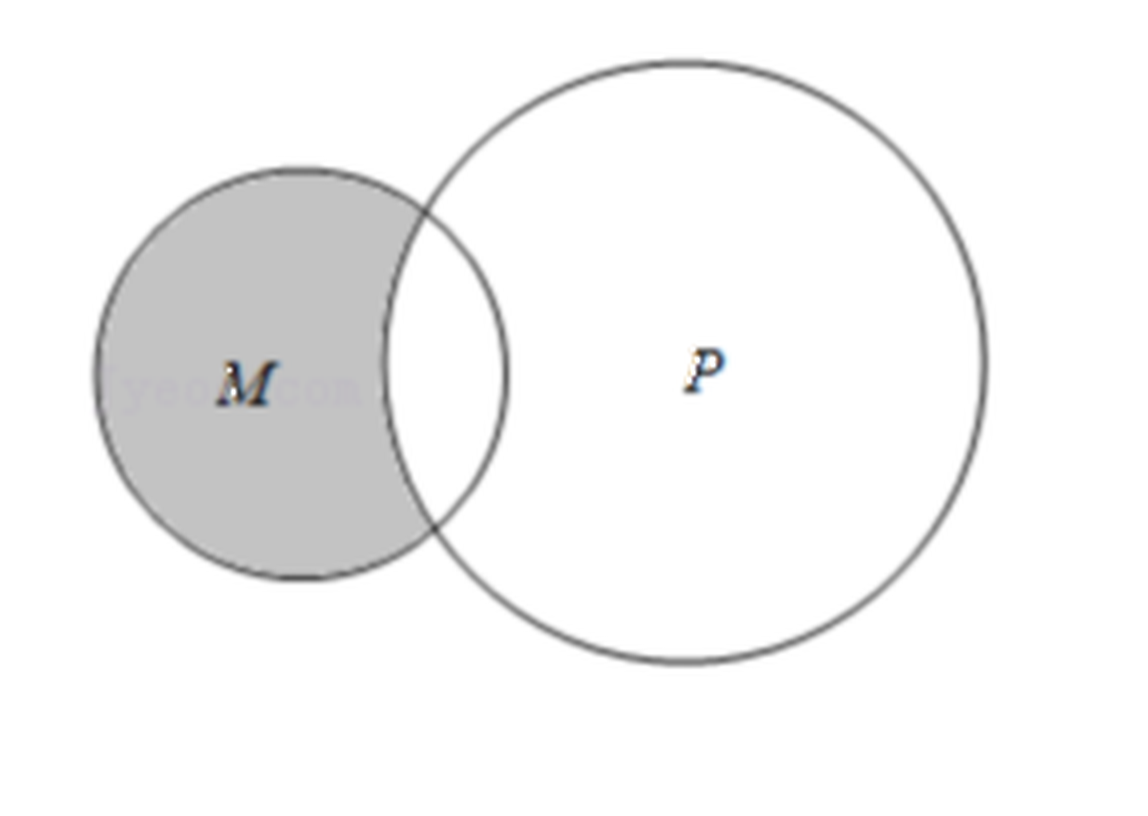
\includegraphics[width=0.36\textwidth]{figures/venn_M_shaded_P.png}
\end{center}

\step{阴影部分表示 $M-P$，所以 $M-(M-P)=M\cap P$. 故选 $B$.}
\solend

\fi

\item 设 $A_1$、$A_2$、$\cdots$、$A_7$ 均是含有 2 个元素的集合，且满足：

$A_i\cap A_{i+1}=\varnothing(i=1,2,3,4,5,6)$，$A_1\cap A_7=\varnothing$. 记 $B=A_1\cup A_2\cup\cdots\cup A_7$，则 $B$ 中元素个数的最小值是\mbox{（\quad）}

\keepwithprev
A. $4$\qquad B. $5$\qquad C. $6$\qquad D. $7$

\ans{$B$}

\ifanswer
\solbegin
\step{$A_1\cap A_7=\varnothing$，$A_i\cap A_{i+1}=\varnothing(i=1,2,3,4,5,6)$，}
\step{所以 $A_1$ 与 $A_2$ 的元素不同，则 $A_1\cup A_2$ 元素个数为 $4$，}
\step{若 $B$ 中元素个数的最小值是 $4$，则只能是 $A_3=A_1=A_5=A_7$，$A_4=A_2=A_6$，}
\step{与 $A_1\cap A_7=\varnothing$ 矛盾，}
\step{若 $A_3$ 从 $A_1$ 中选择 1 个元素，再加入一个新元素，}
\step{这样 $A_1\cup A_2\cup A_3$ 元素个数为 5 个，}
\step{这 5 个元素适当排列，得到 $A_4$、$A_5$、$A_6$、$A_7$，}
\step{例如 $A_1=\{1,2\},A_2=\{3,4\},A_3=\{1,5\}$，}
\step{取 $A_4=\{2,4\},A_5=\{3,5\},A_6=\{1,2\},A_7=\{3,5\}$，符合题意，}
\step{则 $B$ 中元素个数的最小值是 $2+2+1=5$，故选 $B$.}
\solend

\fi

\end{enumerate}

\bigsec{三、解答题}

\begin{enumerate}
\setcounter{enumi}{13}

\item 设 $A=\{x\mid x^2-ax+a^2-19=0\}$，$B=\{x\mid x^2-5x+6=0\}$，$C=\{x\mid x^2+2x-8=0\}$.

\begin{enumerate}[label=(\arabic*)]
\item 若 $A\cap B$ 非空，且 $A\cap C=\varnothing$，求 $a$ 的值；
\item $A\cap B=A\cap C\neq\varnothing$，求 $a$ 的值.
\end{enumerate}

\ifanswer
\solbegin
\stepm{(1)}{由题意，$C=\{-4,2\}$，}
\step{因为 $A\cap B$ 非空且 $A\cap C=\varnothing$，所以 $3\in A$，}
\step{即 $9-3a+a^2-19=0$，解得 $a=-2$ 或 $a=5$，}
\step{当 $a=-2$ 时，$A=\{3,-5\}$，满足题意；}
\step{当 $a=5$ 时，$A=\{2,3\}$，此时 $A\cap C=\{2\}$，不满足题意；}
\step{综上，$a=-2$；}
\stepm{(2)}{因为 $A\cap B=A\cap C\neq\varnothing$，所以 $2\in A$，}
\step{即 $4-2a+a^2-19=0$，解得 $a=-3$ 或 $a=5$，}
\step{当 $a=-3$ 时，$A=\{2,-5\}$，满足题意；}
\step{当 $a=5$ 时，$A=\{2,3\}$，不满足题意，}
\step{故 $a=-3$.}
\solend

\fi

\ansspace[6]

\item 已知 $A=\{x\mid x<-3\text{ 或 }x>1\}$.

\begin{enumerate}[label=(\arabic*)]
\item 若 $B=\{x\mid x<3m+1\text{ 或 }x>m+2\}$，$A\sub B$，求 $m$ 的取值范围.
\item 若 $B=\{x\mid m+2<x<3m+1\}$，$B\sub A$，求 $m$ 的取值范围.
\end{enumerate}

\ifanswer
\solbegin
\stepm{(1)}{当 $3m+1>m+2$，即 $m>\dfrac{1}{2}$ 时，$B=\R$，满足 $A\sub B$；}
\step{当 $3m+1\leqslant m+2$，即 $m\leqslant\dfrac{1}{2}$ 时，要使 $A\sub B$，}
\step{得 $\begin{cases}3m+1\geqslant-3\text{ ①}\\ m+2\leqslant 1\text{ ②}\end{cases}$，解得 $-\dfrac{4}{3}\leqslant m\leqslant-1$.}
\step{综上所述，$m$ 的取值范围为 $\left\{m\mid -\dfrac{4}{3}\leqslant m\leqslant-1\text{ 或 }m>\dfrac{1}{2}\right\}$；}
\stepm{(2)}{当 $B=\varnothing$ 时，则 $3m+1\leqslant m+2$，即 $m\leqslant\dfrac{1}{2}$ 时，满足 $B\sub A$；}
\step{当 $B\neq\varnothing$ 时，且 $B\sub A$，则 $\begin{cases}3m+1>m+2\\ 3m+1\leqslant-3\text{ 或 }m+2\geqslant 1\end{cases}$，所以 $m>\dfrac{1}{2}$.}
\step{综上所述，$m$ 的取值范围为 $\R$.}
\solend

\fi

\ansspace[6]

% 压轴题：其后已无内容，故作答区全用可丢弃胶水（\ansspace*），并在题目前先量一下版面。
\ansneed{7cm}

\item 已知集合 $A$ 为非空集合，定义

$S=\{x\mid x=a+b,a,b\in A\},T=\{x\mid x=|a-b|,a,b\in A\}$.

\begin{enumerate}[label=(\arabic*)]
\item 若集合 $A=\{1,3\}$，直接写出集合 $S$、$T$（无需写计算过程）；
\item 若集合 $A=\{x_1,x_2,x_3,x_4\}$，$x_1<x_2<x_3<x_4$，且 $T=A$，求证：$x_1+x_4=x_2+x_3$；
\item 若集合 $A=\{x\mid 0\leqslant x\leqslant 2021,x\in\N\}$，$S\cap T=\varnothing$. 记 $|A|$ 为集合 $A$ 中元素的个数，求 $|A|$ 的最大值.
\end{enumerate}

\ifanswer
\solbegin
\stepm{(1)}{$S=\{2,4,6\},T=\{0,2\}$；}
\stepm{(2)}{集合 $T$ 中最小的元素为 0，因为 $T=A$，且 $x_1<x_2<x_3<x_4$，所以 $x_1=0$，}
\step{所以集合 $T$ 中元素为 $x_2-x_1=x_2,x_3-x_1=x_3,x_4-x_1=x_4$，}
\step{以及 $x_3-x_2,x_4-x_2,x_4-x_3$ 均属于 $A$，}
% 注：本行原卷印「所以 $x_3$ 即 $x_4-x_2=x_3-x_1$」，「所以 $x_3$ 即 …」语义不完整，
%     疑有漏排（按本段结论应得 $x_4-x_2=x_3$），无法确证原意，本稿照抄原卷、未改。
\step{因为 $x_1=0<x_3-x_2<x_4-x_2<x_4$，所以 $x_3$ 即 $x_4-x_2=x_3-x_1$，}
\step{即 $x_1+x_4=x_2+x_3$；}
\stepm{(3)}{设 $A=\{a_1,a_2,a_3,\cdots,a_k\}$ 满足题意，其中 $a_1<a_2<\cdots<a_k$，}
\step{则 $2a_1<a_1+a_2<\cdots<a_1+a_k<a_2+a_k<a_3+a_k<\cdots<a_{k-1}+a_k<2a_k$，}
\step{所以 $|S\cup T|\leqslant 2k+1$，所以 $3k-1\leqslant 2a_k+1\leqslant 4043(k\in\N^*)$，}
\step{所以 $k\leqslant 1348$，}
\step{实际上当 $A=\{674,675,676,\cdots,2021\}$ 时满足题意，}
\step{证明如下：设 $A=\{m,m+1,m+2,\cdots,2021\},m\in\N$，}
\step{设 $S=\{2m,2m+1,2m+2,\cdots,4042\}$，$T=\{0,1,2,\cdots,2021-m\}$，}
\step{由题意得 $2021-m<2m$，即 $m>673\dfrac{2}{3}$，}
\step{故 $m$ 的最小值是 674，于是当 $m=674$，$A$ 中的元素最多，}
\step{即 $A=\{674,675,676,\cdots,2021\}$ 时满足题意，}
\step{综上所述，集合 $A$ 中元素的个数的最大值是 $1348$.}
\solend

\fi

\ansspace*[9]

\end{enumerate}

\bigsec{附加题}

\begin{enumerate}
\setcounter{enumi}{16}

\item 设 $A$ 是整数集的一个非空子集，对于 $k\in A$，如果 $k-1\notin A$ 且 $k+1\notin A$，那么 $k$ 是 $A$ 的一个“孤立元”。给定 $S=\{1,2,3,4,5,6,7,8\}$，由 $S$ 的 3 个元素构成的所有集合中，不含“孤立元”的集合共有 \blankline[2.4em] 个.

\ifanswer
\solbegin
\step{由题意得，“孤立元”即为在集合中无与之相邻的元素，}
\step{满足条件的集合有 $\{1,2,3\},\{2,3,4\},\{3,4,5\},\{4,5,6\},\{5,6,7\},\{6,7,8\}$，}
\step{共 6 个集合.}
\solend

\fi

\item 已知 $A\cap B=\varnothing$，$M=\{T\mid T\sub A\}$，$P=\{S\mid S\sub B\}$，则 $M\cap P=$ \blankline[4.4em].

\ans{$\{\varnothing\}$}

\item 已知集合 $A=\{x\mid x=m^2-n^2,m,n\in\Z\}$，写出所有满足集合 $A$ 的偶数 \blankline[4.4em].

\ans{$4n,n\in\Z$}

\item 对于给定的正整数 $n(n\geqslant 2)$ 若有限集合 $A=\{a_1,a_2,\cdots,a_n\}\sub M$，且满足

$a_1+a_2+\cdots+a_n=a_1\cdot a_2\cdots a_n$，则称 $A$ 为集合 $M$ 的 $n$ 元“调和子集”，则自然数集 $\N$ 的所有 3 元“调和子集”为 \blankline[3.6em].

\ans{$\{1,2,3\}$}

\end{enumerate}

\end{document}
"
%
% 原始材料是微信公众号图文（公众号「魔都数学加油站」），正文为 7 张 PNG 页（1080×1527）。
% 原文本身就是一份**讲评版**——题目下方直接印出【答案】或【解析】。试题文字、答案与解析
% 均照原卷录入，未改内容。卷面上的粉色斜水印「魔都数学加油站」属水印，未录入。
%
% 卷首标题：原卷印作「2026-2027 年七宝中学高一上抱孩子练习 9.8」——「抱孩子练习」四字
% 确系原卷所印（已放大 imgs_B/00.png 卷首核对），句末的「9.8」亦印在同一标题行内，
% 本稿一并照录，未改作「周末作业」；年份区间按全稿惯例排 en dash。
%
% 与原卷的排版差异（均已在 README「说明」中交代）：
%   ① 原文自**第 3 题**起（第 1、2 题未在该文中发布），故本稿题号亦自 3 起；
%   ② 原卷本就印有「一、填空题」「二、选择题」「三、解答题」三节标题，末节另印「附加题」，
%      本稿照原卷分节，只把标题改排成全稿统一的「大节标题」样式；
%   ③ 原卷填空、选择的答案直接印在题目下方，本稿统一改为试卷版隐去、答案版以【答案】或
%      【解析】给出（第 11 题原卷的答案是写在解析末句「故选 B」里的），使两版彻底分离；
%   ④ 原卷的集合符号 $R$、$Z$、$N$ 有正体与粗体两种写法（第 4 题的 $\mathbf{R}$、
%      第 16(3)、17、19、20 题的 $\mathbf{N}$、$\mathbf{Z}$ 为粗体，第 15 题解析的 $B=R$
%      为正体），本稿按全稿惯例统一写作 $\R$、$\Z$、$\N$；
%   ⑤ 原卷用**半角**括号（第 13 题「$\varnothing(i=1,2,3,4,5,6)$」、第 16(1)「(无需写计算过程)」、
%      第 16(2)「$A=\{x_1,x_2,x_3,x_4\}$」、第 20 题「$n(n\geqslant 2)$」），本稿按全稿惯例排全角；
%   ⑥ 原卷未印副标题，本稿按全稿惯例补出副标题「集合与常用逻辑用语」；
%   ⑦ 第 18、20 题的 $\subseteq$（带下划线，真包含写作 $\subset$ 与之形近）已逐处放大比对确认，
%      第 18 题的答案 $\{\varnothing\}$ 亦与 $\subseteq$ 口径相符（若为真包含则答案应为 $\varnothing$）。
%
% 原卷存疑两处（均已放大到能看清字形后核对，无法确证原意，本稿照抄原卷、未改）：
%   ① 第 10 题【解析】末句原卷印「所以 $1-k^2\neq 0$，即 $k\neq\pm 1$」——按此式，当 $k=1$
%      时两方程为同一直线、有无穷多解，$A\cap B\neq\varnothing$ 仍成立，故 $A\cap B\neq\varnothing$
%      当且仅当 $k\neq -1$；原卷结论与题设不合，疑为原卷笔误，但无法确证原意，本稿照抄原卷；
%   ② 第 16(2)【解析】原卷印「因为 $x_1=0<x_3-x_2<x_4-x_2<x_4$，所以 $x_3$ 即 $x_4-x_2=x_3-x_1$，」
%      ——「所以 $x_3$ 即 …」一句语义不完整，疑有漏排（按本段结论应得 $x_4-x_2=x_3$），
%      无法确证原意，本稿照抄原卷。

\documentclass[a4paper,11pt]{article}
\usepackage{common}

\begin{document}

\examtitlest[3]{2026--2027 年七宝中学高一上抱孩子练习 9.8}{集合与常用逻辑用语}

\bigsec{一、填空题}

\begin{enumerate}
\setcounter{enumi}{2}

\item 方程 $\sqrt{x+2}=-x$ 的解的集合为 \blankline[4.4em].

\ifanswer
\solbegin
\step{因为 $\sqrt{x+2}=-x$，所以 $\begin{cases}x\leqslant 0\\ x+2=x^2\end{cases}$，解得 $x=-1$，}
\step{所以方程 $\sqrt{x+2}=-x$ 的解的集合为 $\{-1\}$.}
\solend

\fi

\item 若 $A=\{x\mid a-4<x\leqslant a+4\}$，$B=\{x\mid x>5\text{ 或 }x<-1\}$，且 $A\cup B=\R$，则实数 $a$ 的取值范围是 \blankline[3.6em].

\ans{$[1,3)$}

\item 设集合 $A=\{x\mid x=2n+1,n\in\N\}$，$B=\{x\mid x=3n,n\in\N\}$，则 $A\cap B=$ \blankline[4.4em].

\ans{$\{x\mid x=6n+3,n\in\N\}$}

\item 已知集合 $A=\{1,2\}$，集合 $B=\{x\mid ax=6\}$，若 $A\cup B=A$，则 $a$ 的所有取值构成的集合为 \blankline[4.4em].

\ifanswer
\solbegin
\step{因为 $A\cup B=A$，所以 $B\sub A$，}
\step{当 $a=0$ 时，$B=\varnothing$，满足 $B\sub A$；}
\step{当 $a\neq 0$ 时，$B=\left\{\dfrac{6}{a}\right\}$，则 $\dfrac{6}{a}=1$ 或 $\dfrac{6}{a}=2$，解得 $a=6$ 或 $a=3$，}
\step{综上所述，$a$ 的所有取值构成的集合为 $\{0,3,6\}$.}
\solend

\fi

\item 设 $U=\{2,4,a^2-a+1\}$，$A=\{2,|a+1|\}$，$\overline{A}=\{7\}$，则 $a=$ \blankline[2.4em].

\ans{$3$}

\item 已知集合 $A=\{x\mid x^2-px-q=0\}$，$B=\{x\mid x^2+qx-p=0\}$，且 $A\cap B=\{1\}$，则 $A\cup B=$ \blankline[4.4em].

\ans{$\{0,-1,1\}$}

\item 定义集合运算：$A\odot B=\{z\mid z=xy(x+y),x\in A,y\in B\}$，若 $A=\{1,2\},B=\{3,4\}$，则 $A\odot B$ 的所有元素之和是 \blankline[3.6em].

\ans{$110$}

\item 已知集合 $A=\{(x,y)\mid kx+y=k+1\}$，$B=\{(x,y)\mid x+ky=2k\}$，其中 $k$ 为实数，$A\cap B\neq\varnothing$，则 $k$ 的取值范围是 \blankline[4.4em].

\ifanswer
\solbegin
\step{因为 $A\cap B\neq\varnothing$，所以方程组 $\begin{cases}kx+y=k+1\\ x+ky=2k\end{cases}$ 有解，消 $y$ 得 $(1-k^2)x=k-k^2$，}
% 注：末句原卷印「所以 $1-k^2\neq 0$，即 $k\neq\pm 1$」。按此式，$k=1$ 时两方程为同一直线、
%     有无穷多解，$A\cap B\neq\varnothing$ 仍成立，故结论应为 $k\neq -1$。疑为原卷笔误，
%     但无法确证原意，本稿照抄原卷、未改（详见文件头「原卷存疑」①）。
\step{所以 $1-k^2\neq 0$，即 $k\neq\pm 1$.}
\solend

\fi

\end{enumerate}

\bigsec{二、选择题}

\begin{enumerate}
\setcounter{enumi}{10}

\item 给出关系式：①$0\in\varnothing$；②$\varnothing=\{0\}$；③$\{a,b\}=\{b,a\}$；④$\{y\mid y=x^2-2\}=\{(x,y)\mid y=x^2-2\}$，其中正确的关系式的个数是\mbox{（\quad）}

\keepwithprev
A. $0$\qquad B. $1$\qquad C. $2$\qquad D. $3$

\ans{$B$}

\ifanswer
\solbegin
\step{在①中，$\varnothing$ 表示空集，$0\notin\varnothing$，故①错误；在②中，$\varnothing\sub\{0\}$，故②错误；}
\step{在③中，$\{a,b\}=\{b,a\}$，故③正确；}
\step{在④中，因为，$\{y\mid y=x^2-2\}$ 和 $\{(x,y)\mid y=x^2-2\}$ 的代表元素不同，}
\step{所以 $\{y\mid y=x^2-2\}\neq\{(x,y)\mid y=x^2-2\}$，故④错误.}
\step{故正确的是③，故选 $B$.}
\solend

\fi

\item 设集合 $M$、$P\neq\varnothing$，定义集合 $M-P=\{x\mid x\in M,x\notin P\}$，则集合 $M-(M-P)$ 是\mbox{（\quad）}

\keepwithprev
A. $P$\qquad B. $M$\qquad C. $M\cup P$\qquad D. $M\cap P$

\ans{$B$}

\ifanswer
\solbegin
\step{$M-(M-P)=\{x\mid x\in M,\text{ 且 }x\notin(M-P)\}$，}
\step{用 venn 图表示集合 $M$、$P$ 的关系如图：}

\begin{center}
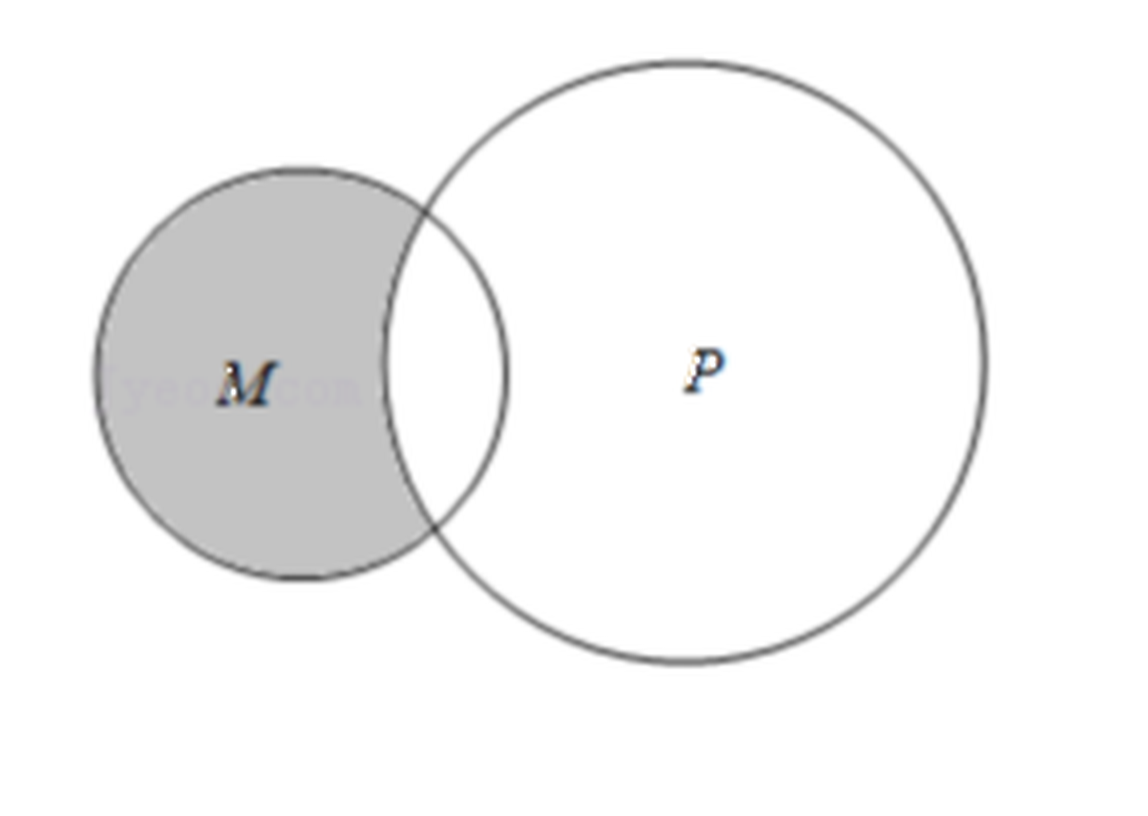
\includegraphics[width=0.36\textwidth]{figures/venn_M_shaded_P.png}
\end{center}

\step{阴影部分表示 $M-P$，所以 $M-(M-P)=M\cap P$. 故选 $B$.}
\solend

\fi

\item 设 $A_1$、$A_2$、$\cdots$、$A_7$ 均是含有 2 个元素的集合，且满足：

$A_i\cap A_{i+1}=\varnothing(i=1,2,3,4,5,6)$，$A_1\cap A_7=\varnothing$. 记 $B=A_1\cup A_2\cup\cdots\cup A_7$，则 $B$ 中元素个数的最小值是\mbox{（\quad）}

\keepwithprev
A. $4$\qquad B. $5$\qquad C. $6$\qquad D. $7$

\ans{$B$}

\ifanswer
\solbegin
\step{$A_1\cap A_7=\varnothing$，$A_i\cap A_{i+1}=\varnothing(i=1,2,3,4,5,6)$，}
\step{所以 $A_1$ 与 $A_2$ 的元素不同，则 $A_1\cup A_2$ 元素个数为 $4$，}
\step{若 $B$ 中元素个数的最小值是 $4$，则只能是 $A_3=A_1=A_5=A_7$，$A_4=A_2=A_6$，}
\step{与 $A_1\cap A_7=\varnothing$ 矛盾，}
\step{若 $A_3$ 从 $A_1$ 中选择 1 个元素，再加入一个新元素，}
\step{这样 $A_1\cup A_2\cup A_3$ 元素个数为 5 个，}
\step{这 5 个元素适当排列，得到 $A_4$、$A_5$、$A_6$、$A_7$，}
\step{例如 $A_1=\{1,2\},A_2=\{3,4\},A_3=\{1,5\}$，}
\step{取 $A_4=\{2,4\},A_5=\{3,5\},A_6=\{1,2\},A_7=\{3,5\}$，符合题意，}
\step{则 $B$ 中元素个数的最小值是 $2+2+1=5$，故选 $B$.}
\solend

\fi

\end{enumerate}

\bigsec{三、解答题}

\begin{enumerate}
\setcounter{enumi}{13}

\item 设 $A=\{x\mid x^2-ax+a^2-19=0\}$，$B=\{x\mid x^2-5x+6=0\}$，$C=\{x\mid x^2+2x-8=0\}$.

\begin{enumerate}[label=(\arabic*)]
\item 若 $A\cap B$ 非空，且 $A\cap C=\varnothing$，求 $a$ 的值；
\item $A\cap B=A\cap C\neq\varnothing$，求 $a$ 的值.
\end{enumerate}

\ifanswer
\solbegin
\stepm{(1)}{由题意，$C=\{-4,2\}$，}
\step{因为 $A\cap B$ 非空且 $A\cap C=\varnothing$，所以 $3\in A$，}
\step{即 $9-3a+a^2-19=0$，解得 $a=-2$ 或 $a=5$，}
\step{当 $a=-2$ 时，$A=\{3,-5\}$，满足题意；}
\step{当 $a=5$ 时，$A=\{2,3\}$，此时 $A\cap C=\{2\}$，不满足题意；}
\step{综上，$a=-2$；}
\stepm{(2)}{因为 $A\cap B=A\cap C\neq\varnothing$，所以 $2\in A$，}
\step{即 $4-2a+a^2-19=0$，解得 $a=-3$ 或 $a=5$，}
\step{当 $a=-3$ 时，$A=\{2,-5\}$，满足题意；}
\step{当 $a=5$ 时，$A=\{2,3\}$，不满足题意，}
\step{故 $a=-3$.}
\solend

\fi

\ansspace[6]

\item 已知 $A=\{x\mid x<-3\text{ 或 }x>1\}$.

\begin{enumerate}[label=(\arabic*)]
\item 若 $B=\{x\mid x<3m+1\text{ 或 }x>m+2\}$，$A\sub B$，求 $m$ 的取值范围.
\item 若 $B=\{x\mid m+2<x<3m+1\}$，$B\sub A$，求 $m$ 的取值范围.
\end{enumerate}

\ifanswer
\solbegin
\stepm{(1)}{当 $3m+1>m+2$，即 $m>\dfrac{1}{2}$ 时，$B=\R$，满足 $A\sub B$；}
\step{当 $3m+1\leqslant m+2$，即 $m\leqslant\dfrac{1}{2}$ 时，要使 $A\sub B$，}
\step{得 $\begin{cases}3m+1\geqslant-3\text{ ①}\\ m+2\leqslant 1\text{ ②}\end{cases}$，解得 $-\dfrac{4}{3}\leqslant m\leqslant-1$.}
\step{综上所述，$m$ 的取值范围为 $\left\{m\mid -\dfrac{4}{3}\leqslant m\leqslant-1\text{ 或 }m>\dfrac{1}{2}\right\}$；}
\stepm{(2)}{当 $B=\varnothing$ 时，则 $3m+1\leqslant m+2$，即 $m\leqslant\dfrac{1}{2}$ 时，满足 $B\sub A$；}
\step{当 $B\neq\varnothing$ 时，且 $B\sub A$，则 $\begin{cases}3m+1>m+2\\ 3m+1\leqslant-3\text{ 或 }m+2\geqslant 1\end{cases}$，所以 $m>\dfrac{1}{2}$.}
\step{综上所述，$m$ 的取值范围为 $\R$.}
\solend

\fi

\ansspace[6]

% 压轴题：其后已无内容，故作答区全用可丢弃胶水（\ansspace*），并在题目前先量一下版面。
\ansneed{7cm}

\item 已知集合 $A$ 为非空集合，定义

$S=\{x\mid x=a+b,a,b\in A\},T=\{x\mid x=|a-b|,a,b\in A\}$.

\begin{enumerate}[label=(\arabic*)]
\item 若集合 $A=\{1,3\}$，直接写出集合 $S$、$T$（无需写计算过程）；
\item 若集合 $A=\{x_1,x_2,x_3,x_4\}$，$x_1<x_2<x_3<x_4$，且 $T=A$，求证：$x_1+x_4=x_2+x_3$；
\item 若集合 $A=\{x\mid 0\leqslant x\leqslant 2021,x\in\N\}$，$S\cap T=\varnothing$. 记 $|A|$ 为集合 $A$ 中元素的个数，求 $|A|$ 的最大值.
\end{enumerate}

\ifanswer
\solbegin
\stepm{(1)}{$S=\{2,4,6\},T=\{0,2\}$；}
\stepm{(2)}{集合 $T$ 中最小的元素为 0，因为 $T=A$，且 $x_1<x_2<x_3<x_4$，所以 $x_1=0$，}
\step{所以集合 $T$ 中元素为 $x_2-x_1=x_2,x_3-x_1=x_3,x_4-x_1=x_4$，}
\step{以及 $x_3-x_2,x_4-x_2,x_4-x_3$ 均属于 $A$，}
% 注：本行原卷印「所以 $x_3$ 即 $x_4-x_2=x_3-x_1$」，「所以 $x_3$ 即 …」语义不完整，
%     疑有漏排（按本段结论应得 $x_4-x_2=x_3$），无法确证原意，本稿照抄原卷、未改。
\step{因为 $x_1=0<x_3-x_2<x_4-x_2<x_4$，所以 $x_3$ 即 $x_4-x_2=x_3-x_1$，}
\step{即 $x_1+x_4=x_2+x_3$；}
\stepm{(3)}{设 $A=\{a_1,a_2,a_3,\cdots,a_k\}$ 满足题意，其中 $a_1<a_2<\cdots<a_k$，}
\step{则 $2a_1<a_1+a_2<\cdots<a_1+a_k<a_2+a_k<a_3+a_k<\cdots<a_{k-1}+a_k<2a_k$，}
\step{所以 $|S\cup T|\leqslant 2k+1$，所以 $3k-1\leqslant 2a_k+1\leqslant 4043(k\in\N^*)$，}
\step{所以 $k\leqslant 1348$，}
\step{实际上当 $A=\{674,675,676,\cdots,2021\}$ 时满足题意，}
\step{证明如下：设 $A=\{m,m+1,m+2,\cdots,2021\},m\in\N$，}
\step{设 $S=\{2m,2m+1,2m+2,\cdots,4042\}$，$T=\{0,1,2,\cdots,2021-m\}$，}
\step{由题意得 $2021-m<2m$，即 $m>673\dfrac{2}{3}$，}
\step{故 $m$ 的最小值是 674，于是当 $m=674$，$A$ 中的元素最多，}
\step{即 $A=\{674,675,676,\cdots,2021\}$ 时满足题意，}
\step{综上所述，集合 $A$ 中元素的个数的最大值是 $1348$.}
\solend

\fi

\ansspace*[9]

\end{enumerate}

\bigsec{附加题}

\begin{enumerate}
\setcounter{enumi}{16}

\item 设 $A$ 是整数集的一个非空子集，对于 $k\in A$，如果 $k-1\notin A$ 且 $k+1\notin A$，那么 $k$ 是 $A$ 的一个“孤立元”。给定 $S=\{1,2,3,4,5,6,7,8\}$，由 $S$ 的 3 个元素构成的所有集合中，不含“孤立元”的集合共有 \blankline[2.4em] 个.

\ifanswer
\solbegin
\step{由题意得，“孤立元”即为在集合中无与之相邻的元素，}
\step{满足条件的集合有 $\{1,2,3\},\{2,3,4\},\{3,4,5\},\{4,5,6\},\{5,6,7\},\{6,7,8\}$，}
\step{共 6 个集合.}
\solend

\fi

\item 已知 $A\cap B=\varnothing$，$M=\{T\mid T\sub A\}$，$P=\{S\mid S\sub B\}$，则 $M\cap P=$ \blankline[4.4em].

\ans{$\{\varnothing\}$}

\item 已知集合 $A=\{x\mid x=m^2-n^2,m,n\in\Z\}$，写出所有满足集合 $A$ 的偶数 \blankline[4.4em].

\ans{$4n,n\in\Z$}

\item 对于给定的正整数 $n(n\geqslant 2)$ 若有限集合 $A=\{a_1,a_2,\cdots,a_n\}\sub M$，且满足

$a_1+a_2+\cdots+a_n=a_1\cdot a_2\cdots a_n$，则称 $A$ 为集合 $M$ 的 $n$ 元“调和子集”，则自然数集 $\N$ 的所有 3 元“调和子集”为 \blankline[3.6em].

\ans{$\{1,2,3\}$}

\end{enumerate}

\end{document}
"
%
% 原始材料是微信公众号图文（公众号「魔都数学加油站」），正文为 7 张 PNG 页（1080×1527）。
% 原文本身就是一份**讲评版**——题目下方直接印出【答案】或【解析】。试题文字、答案与解析
% 均照原卷录入，未改内容。卷面上的粉色斜水印「魔都数学加油站」属水印，未录入。
%
% 卷首标题：原卷印作「2026-2027 年七宝中学高一上抱孩子练习 9.8」——「抱孩子练习」四字
% 确系原卷所印（已放大 imgs_B/00.png 卷首核对），句末的「9.8」亦印在同一标题行内，
% 本稿一并照录，未改作「周末作业」；年份区间按全稿惯例排 en dash。
%
% 与原卷的排版差异（均已在 README「说明」中交代）：
%   ① 原文自**第 3 题**起（第 1、2 题未在该文中发布），故本稿题号亦自 3 起；
%   ② 原卷本就印有「一、填空题」「二、选择题」「三、解答题」三节标题，末节另印「附加题」，
%      本稿照原卷分节，只把标题改排成全稿统一的「大节标题」样式；
%   ③ 原卷填空、选择的答案直接印在题目下方，本稿统一改为试卷版隐去、答案版以【答案】或
%      【解析】给出（第 11 题原卷的答案是写在解析末句「故选 B」里的），使两版彻底分离；
%   ④ 原卷的集合符号 $R$、$Z$、$N$ 有正体与粗体两种写法（第 4 题的 $\mathbf{R}$、
%      第 16(3)、17、19、20 题的 $\mathbf{N}$、$\mathbf{Z}$ 为粗体，第 15 题解析的 $B=R$
%      为正体），本稿按全稿惯例统一写作 $\R$、$\Z$、$\N$；
%   ⑤ 原卷用**半角**括号（第 13 题「$\varnothing(i=1,2,3,4,5,6)$」、第 16(1)「(无需写计算过程)」、
%      第 16(2)「$A=\{x_1,x_2,x_3,x_4\}$」、第 20 题「$n(n\geqslant 2)$」），本稿按全稿惯例排全角；
%   ⑥ 原卷未印副标题，本稿按全稿惯例补出副标题「集合与常用逻辑用语」；
%   ⑦ 第 18、20 题的 $\subseteq$（带下划线，真包含写作 $\subset$ 与之形近）已逐处放大比对确认，
%      第 18 题的答案 $\{\varnothing\}$ 亦与 $\subseteq$ 口径相符（若为真包含则答案应为 $\varnothing$）。
%
% 原卷存疑两处（均已放大到能看清字形后核对，无法确证原意，本稿照抄原卷、未改）：
%   ① 第 10 题【解析】末句原卷印「所以 $1-k^2\neq 0$，即 $k\neq\pm 1$」——按此式，当 $k=1$
%      时两方程为同一直线、有无穷多解，$A\cap B\neq\varnothing$ 仍成立，故 $A\cap B\neq\varnothing$
%      当且仅当 $k\neq -1$；原卷结论与题设不合，疑为原卷笔误，但无法确证原意，本稿照抄原卷；
%   ② 第 16(2)【解析】原卷印「因为 $x_1=0<x_3-x_2<x_4-x_2<x_4$，所以 $x_3$ 即 $x_4-x_2=x_3-x_1$，」
%      ——「所以 $x_3$ 即 …」一句语义不完整，疑有漏排（按本段结论应得 $x_4-x_2=x_3$），
%      无法确证原意，本稿照抄原卷。

\documentclass[a4paper,11pt]{article}
\usepackage{common}

\begin{document}

\examtitlest[3]{2026--2027 年七宝中学高一上抱孩子练习 9.8}{集合与常用逻辑用语}

\bigsec{一、填空题}

\begin{enumerate}
\setcounter{enumi}{2}

\item 方程 $\sqrt{x+2}=-x$ 的解的集合为 \blankline[4.4em].

\ifanswer
\solbegin
\step{因为 $\sqrt{x+2}=-x$，所以 $\begin{cases}x\leqslant 0\\ x+2=x^2\end{cases}$，解得 $x=-1$，}
\step{所以方程 $\sqrt{x+2}=-x$ 的解的集合为 $\{-1\}$.}
\solend

\fi

\item 若 $A=\{x\mid a-4<x\leqslant a+4\}$，$B=\{x\mid x>5\text{ 或 }x<-1\}$，且 $A\cup B=\R$，则实数 $a$ 的取值范围是 \blankline[3.6em].

\ans{$[1,3)$}

\item 设集合 $A=\{x\mid x=2n+1,n\in\N\}$，$B=\{x\mid x=3n,n\in\N\}$，则 $A\cap B=$ \blankline[4.4em].

\ans{$\{x\mid x=6n+3,n\in\N\}$}

\item 已知集合 $A=\{1,2\}$，集合 $B=\{x\mid ax=6\}$，若 $A\cup B=A$，则 $a$ 的所有取值构成的集合为 \blankline[4.4em].

\ifanswer
\solbegin
\step{因为 $A\cup B=A$，所以 $B\sub A$，}
\step{当 $a=0$ 时，$B=\varnothing$，满足 $B\sub A$；}
\step{当 $a\neq 0$ 时，$B=\left\{\dfrac{6}{a}\right\}$，则 $\dfrac{6}{a}=1$ 或 $\dfrac{6}{a}=2$，解得 $a=6$ 或 $a=3$，}
\step{综上所述，$a$ 的所有取值构成的集合为 $\{0,3,6\}$.}
\solend

\fi

\item 设 $U=\{2,4,a^2-a+1\}$，$A=\{2,|a+1|\}$，$\overline{A}=\{7\}$，则 $a=$ \blankline[2.4em].

\ans{$3$}

\item 已知集合 $A=\{x\mid x^2-px-q=0\}$，$B=\{x\mid x^2+qx-p=0\}$，且 $A\cap B=\{1\}$，则 $A\cup B=$ \blankline[4.4em].

\ans{$\{0,-1,1\}$}

\item 定义集合运算：$A\odot B=\{z\mid z=xy(x+y),x\in A,y\in B\}$，若 $A=\{1,2\},B=\{3,4\}$，则 $A\odot B$ 的所有元素之和是 \blankline[3.6em].

\ans{$110$}

\item 已知集合 $A=\{(x,y)\mid kx+y=k+1\}$，$B=\{(x,y)\mid x+ky=2k\}$，其中 $k$ 为实数，$A\cap B\neq\varnothing$，则 $k$ 的取值范围是 \blankline[4.4em].

\ifanswer
\solbegin
\step{因为 $A\cap B\neq\varnothing$，所以方程组 $\begin{cases}kx+y=k+1\\ x+ky=2k\end{cases}$ 有解，消 $y$ 得 $(1-k^2)x=k-k^2$，}
% 注：末句原卷印「所以 $1-k^2\neq 0$，即 $k\neq\pm 1$」。按此式，$k=1$ 时两方程为同一直线、
%     有无穷多解，$A\cap B\neq\varnothing$ 仍成立，故结论应为 $k\neq -1$。疑为原卷笔误，
%     但无法确证原意，本稿照抄原卷、未改（详见文件头「原卷存疑」①）。
\step{所以 $1-k^2\neq 0$，即 $k\neq\pm 1$.}
\solend

\fi

\end{enumerate}

\bigsec{二、选择题}

\begin{enumerate}
\setcounter{enumi}{10}

\item 给出关系式：①$0\in\varnothing$；②$\varnothing=\{0\}$；③$\{a,b\}=\{b,a\}$；④$\{y\mid y=x^2-2\}=\{(x,y)\mid y=x^2-2\}$，其中正确的关系式的个数是\mbox{（\quad）}

\keepwithprev
A. $0$\qquad B. $1$\qquad C. $2$\qquad D. $3$

\ans{$B$}

\ifanswer
\solbegin
\step{在①中，$\varnothing$ 表示空集，$0\notin\varnothing$，故①错误；在②中，$\varnothing\sub\{0\}$，故②错误；}
\step{在③中，$\{a,b\}=\{b,a\}$，故③正确；}
\step{在④中，因为，$\{y\mid y=x^2-2\}$ 和 $\{(x,y)\mid y=x^2-2\}$ 的代表元素不同，}
\step{所以 $\{y\mid y=x^2-2\}\neq\{(x,y)\mid y=x^2-2\}$，故④错误.}
\step{故正确的是③，故选 $B$.}
\solend

\fi

\item 设集合 $M$、$P\neq\varnothing$，定义集合 $M-P=\{x\mid x\in M,x\notin P\}$，则集合 $M-(M-P)$ 是\mbox{（\quad）}

\keepwithprev
A. $P$\qquad B. $M$\qquad C. $M\cup P$\qquad D. $M\cap P$

\ans{$B$}

\ifanswer
\solbegin
\step{$M-(M-P)=\{x\mid x\in M,\text{ 且 }x\notin(M-P)\}$，}
\step{用 venn 图表示集合 $M$、$P$ 的关系如图：}

\begin{center}
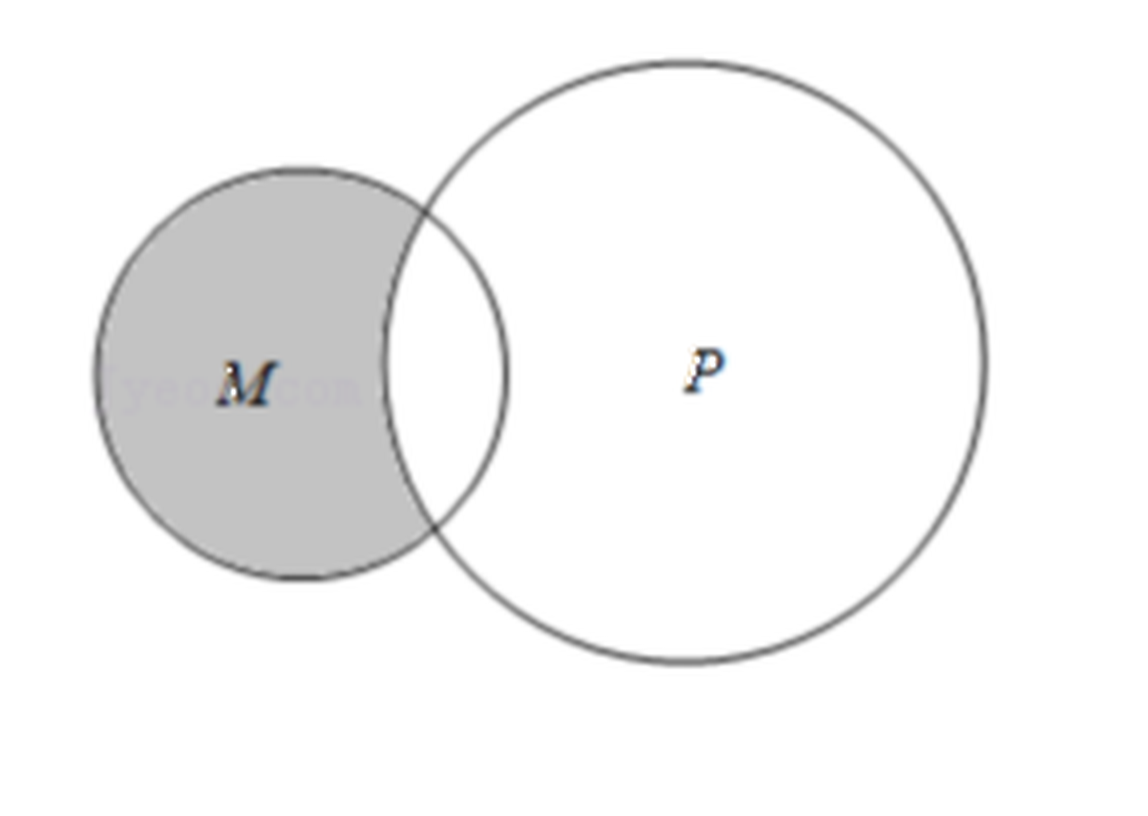
\includegraphics[width=0.36\textwidth]{figures/venn_M_shaded_P.png}
\end{center}

\step{阴影部分表示 $M-P$，所以 $M-(M-P)=M\cap P$. 故选 $B$.}
\solend

\fi

\item 设 $A_1$、$A_2$、$\cdots$、$A_7$ 均是含有 2 个元素的集合，且满足：

$A_i\cap A_{i+1}=\varnothing(i=1,2,3,4,5,6)$，$A_1\cap A_7=\varnothing$. 记 $B=A_1\cup A_2\cup\cdots\cup A_7$，则 $B$ 中元素个数的最小值是\mbox{（\quad）}

\keepwithprev
A. $4$\qquad B. $5$\qquad C. $6$\qquad D. $7$

\ans{$B$}

\ifanswer
\solbegin
\step{$A_1\cap A_7=\varnothing$，$A_i\cap A_{i+1}=\varnothing(i=1,2,3,4,5,6)$，}
\step{所以 $A_1$ 与 $A_2$ 的元素不同，则 $A_1\cup A_2$ 元素个数为 $4$，}
\step{若 $B$ 中元素个数的最小值是 $4$，则只能是 $A_3=A_1=A_5=A_7$，$A_4=A_2=A_6$，}
\step{与 $A_1\cap A_7=\varnothing$ 矛盾，}
\step{若 $A_3$ 从 $A_1$ 中选择 1 个元素，再加入一个新元素，}
\step{这样 $A_1\cup A_2\cup A_3$ 元素个数为 5 个，}
\step{这 5 个元素适当排列，得到 $A_4$、$A_5$、$A_6$、$A_7$，}
\step{例如 $A_1=\{1,2\},A_2=\{3,4\},A_3=\{1,5\}$，}
\step{取 $A_4=\{2,4\},A_5=\{3,5\},A_6=\{1,2\},A_7=\{3,5\}$，符合题意，}
\step{则 $B$ 中元素个数的最小值是 $2+2+1=5$，故选 $B$.}
\solend

\fi

\end{enumerate}

\bigsec{三、解答题}

\begin{enumerate}
\setcounter{enumi}{13}

\item 设 $A=\{x\mid x^2-ax+a^2-19=0\}$，$B=\{x\mid x^2-5x+6=0\}$，$C=\{x\mid x^2+2x-8=0\}$.

\begin{enumerate}[label=(\arabic*)]
\item 若 $A\cap B$ 非空，且 $A\cap C=\varnothing$，求 $a$ 的值；
\item $A\cap B=A\cap C\neq\varnothing$，求 $a$ 的值.
\end{enumerate}

\ifanswer
\solbegin
\stepm{(1)}{由题意，$C=\{-4,2\}$，}
\step{因为 $A\cap B$ 非空且 $A\cap C=\varnothing$，所以 $3\in A$，}
\step{即 $9-3a+a^2-19=0$，解得 $a=-2$ 或 $a=5$，}
\step{当 $a=-2$ 时，$A=\{3,-5\}$，满足题意；}
\step{当 $a=5$ 时，$A=\{2,3\}$，此时 $A\cap C=\{2\}$，不满足题意；}
\step{综上，$a=-2$；}
\stepm{(2)}{因为 $A\cap B=A\cap C\neq\varnothing$，所以 $2\in A$，}
\step{即 $4-2a+a^2-19=0$，解得 $a=-3$ 或 $a=5$，}
\step{当 $a=-3$ 时，$A=\{2,-5\}$，满足题意；}
\step{当 $a=5$ 时，$A=\{2,3\}$，不满足题意，}
\step{故 $a=-3$.}
\solend

\fi

\ansspace[6]

\item 已知 $A=\{x\mid x<-3\text{ 或 }x>1\}$.

\begin{enumerate}[label=(\arabic*)]
\item 若 $B=\{x\mid x<3m+1\text{ 或 }x>m+2\}$，$A\sub B$，求 $m$ 的取值范围.
\item 若 $B=\{x\mid m+2<x<3m+1\}$，$B\sub A$，求 $m$ 的取值范围.
\end{enumerate}

\ifanswer
\solbegin
\stepm{(1)}{当 $3m+1>m+2$，即 $m>\dfrac{1}{2}$ 时，$B=\R$，满足 $A\sub B$；}
\step{当 $3m+1\leqslant m+2$，即 $m\leqslant\dfrac{1}{2}$ 时，要使 $A\sub B$，}
\step{得 $\begin{cases}3m+1\geqslant-3\text{ ①}\\ m+2\leqslant 1\text{ ②}\end{cases}$，解得 $-\dfrac{4}{3}\leqslant m\leqslant-1$.}
\step{综上所述，$m$ 的取值范围为 $\left\{m\mid -\dfrac{4}{3}\leqslant m\leqslant-1\text{ 或 }m>\dfrac{1}{2}\right\}$；}
\stepm{(2)}{当 $B=\varnothing$ 时，则 $3m+1\leqslant m+2$，即 $m\leqslant\dfrac{1}{2}$ 时，满足 $B\sub A$；}
\step{当 $B\neq\varnothing$ 时，且 $B\sub A$，则 $\begin{cases}3m+1>m+2\\ 3m+1\leqslant-3\text{ 或 }m+2\geqslant 1\end{cases}$，所以 $m>\dfrac{1}{2}$.}
\step{综上所述，$m$ 的取值范围为 $\R$.}
\solend

\fi

\ansspace[6]

% 压轴题：其后已无内容，故作答区全用可丢弃胶水（\ansspace*），并在题目前先量一下版面。
\ansneed{7cm}

\item 已知集合 $A$ 为非空集合，定义

$S=\{x\mid x=a+b,a,b\in A\},T=\{x\mid x=|a-b|,a,b\in A\}$.

\begin{enumerate}[label=(\arabic*)]
\item 若集合 $A=\{1,3\}$，直接写出集合 $S$、$T$（无需写计算过程）；
\item 若集合 $A=\{x_1,x_2,x_3,x_4\}$，$x_1<x_2<x_3<x_4$，且 $T=A$，求证：$x_1+x_4=x_2+x_3$；
\item 若集合 $A=\{x\mid 0\leqslant x\leqslant 2021,x\in\N\}$，$S\cap T=\varnothing$. 记 $|A|$ 为集合 $A$ 中元素的个数，求 $|A|$ 的最大值.
\end{enumerate}

\ifanswer
\solbegin
\stepm{(1)}{$S=\{2,4,6\},T=\{0,2\}$；}
\stepm{(2)}{集合 $T$ 中最小的元素为 0，因为 $T=A$，且 $x_1<x_2<x_3<x_4$，所以 $x_1=0$，}
\step{所以集合 $T$ 中元素为 $x_2-x_1=x_2,x_3-x_1=x_3,x_4-x_1=x_4$，}
\step{以及 $x_3-x_2,x_4-x_2,x_4-x_3$ 均属于 $A$，}
% 注：本行原卷印「所以 $x_3$ 即 $x_4-x_2=x_3-x_1$」，「所以 $x_3$ 即 …」语义不完整，
%     疑有漏排（按本段结论应得 $x_4-x_2=x_3$），无法确证原意，本稿照抄原卷、未改。
\step{因为 $x_1=0<x_3-x_2<x_4-x_2<x_4$，所以 $x_3$ 即 $x_4-x_2=x_3-x_1$，}
\step{即 $x_1+x_4=x_2+x_3$；}
\stepm{(3)}{设 $A=\{a_1,a_2,a_3,\cdots,a_k\}$ 满足题意，其中 $a_1<a_2<\cdots<a_k$，}
\step{则 $2a_1<a_1+a_2<\cdots<a_1+a_k<a_2+a_k<a_3+a_k<\cdots<a_{k-1}+a_k<2a_k$，}
\step{所以 $|S\cup T|\leqslant 2k+1$，所以 $3k-1\leqslant 2a_k+1\leqslant 4043(k\in\N^*)$，}
\step{所以 $k\leqslant 1348$，}
\step{实际上当 $A=\{674,675,676,\cdots,2021\}$ 时满足题意，}
\step{证明如下：设 $A=\{m,m+1,m+2,\cdots,2021\},m\in\N$，}
\step{设 $S=\{2m,2m+1,2m+2,\cdots,4042\}$，$T=\{0,1,2,\cdots,2021-m\}$，}
\step{由题意得 $2021-m<2m$，即 $m>673\dfrac{2}{3}$，}
\step{故 $m$ 的最小值是 674，于是当 $m=674$，$A$ 中的元素最多，}
\step{即 $A=\{674,675,676,\cdots,2021\}$ 时满足题意，}
\step{综上所述，集合 $A$ 中元素的个数的最大值是 $1348$.}
\solend

\fi

\ansspace*[9]

\end{enumerate}

\bigsec{附加题}

\begin{enumerate}
\setcounter{enumi}{16}

\item 设 $A$ 是整数集的一个非空子集，对于 $k\in A$，如果 $k-1\notin A$ 且 $k+1\notin A$，那么 $k$ 是 $A$ 的一个“孤立元”。给定 $S=\{1,2,3,4,5,6,7,8\}$，由 $S$ 的 3 个元素构成的所有集合中，不含“孤立元”的集合共有 \blankline[2.4em] 个.

\ifanswer
\solbegin
\step{由题意得，“孤立元”即为在集合中无与之相邻的元素，}
\step{满足条件的集合有 $\{1,2,3\},\{2,3,4\},\{3,4,5\},\{4,5,6\},\{5,6,7\},\{6,7,8\}$，}
\step{共 6 个集合.}
\solend

\fi

\item 已知 $A\cap B=\varnothing$，$M=\{T\mid T\sub A\}$，$P=\{S\mid S\sub B\}$，则 $M\cap P=$ \blankline[4.4em].

\ans{$\{\varnothing\}$}

\item 已知集合 $A=\{x\mid x=m^2-n^2,m,n\in\Z\}$，写出所有满足集合 $A$ 的偶数 \blankline[4.4em].

\ans{$4n,n\in\Z$}

\item 对于给定的正整数 $n(n\geqslant 2)$ 若有限集合 $A=\{a_1,a_2,\cdots,a_n\}\sub M$，且满足

$a_1+a_2+\cdots+a_n=a_1\cdot a_2\cdots a_n$，则称 $A$ 为集合 $M$ 的 $n$ 元“调和子集”，则自然数集 $\N$ 的所有 3 元“调和子集”为 \blankline[3.6em].

\ans{$\{1,2,3\}$}

\end{enumerate}

\end{document}
"
% 紧凑版：xelatex "\def\iscompact{1}% 高一15_七宝中学_抱孩子练习.tex
%   —— 高一上数学「2026-2027 年七宝中学高一上抱孩子练习 9.8」（试卷版/答案版）
% 试卷版：xelatex 高一15_七宝中学_抱孩子练习.tex
% 答案版：xelatex "\def\isanswer{1}% 高一15_七宝中学_抱孩子练习.tex
%   —— 高一上数学「2026-2027 年七宝中学高一上抱孩子练习 9.8」（试卷版/答案版）
% 试卷版：xelatex 高一15_七宝中学_抱孩子练习.tex
% 答案版：xelatex "\def\isanswer{1}% 高一15_七宝中学_抱孩子练习.tex
%   —— 高一上数学「2026-2027 年七宝中学高一上抱孩子练习 9.8」（试卷版/答案版）
% 试卷版：xelatex 高一15_七宝中学_抱孩子练习.tex
% 答案版：xelatex "\def\isanswer{1}\input{高一15_七宝中学_抱孩子练习.tex}"
% 紧凑版：xelatex "\def\iscompact{1}\input{高一15_七宝中学_抱孩子练习.tex}"
%
% 原始材料是微信公众号图文（公众号「魔都数学加油站」），正文为 7 张 PNG 页（1080×1527）。
% 原文本身就是一份**讲评版**——题目下方直接印出【答案】或【解析】。试题文字、答案与解析
% 均照原卷录入，未改内容。卷面上的粉色斜水印「魔都数学加油站」属水印，未录入。
%
% 卷首标题：原卷印作「2026-2027 年七宝中学高一上抱孩子练习 9.8」——「抱孩子练习」四字
% 确系原卷所印（已放大 imgs_B/00.png 卷首核对），句末的「9.8」亦印在同一标题行内，
% 本稿一并照录，未改作「周末作业」；年份区间按全稿惯例排 en dash。
%
% 与原卷的排版差异（均已在 README「说明」中交代）：
%   ① 原文自**第 3 题**起（第 1、2 题未在该文中发布），故本稿题号亦自 3 起；
%   ② 原卷本就印有「一、填空题」「二、选择题」「三、解答题」三节标题，末节另印「附加题」，
%      本稿照原卷分节，只把标题改排成全稿统一的「大节标题」样式；
%   ③ 原卷填空、选择的答案直接印在题目下方，本稿统一改为试卷版隐去、答案版以【答案】或
%      【解析】给出（第 11 题原卷的答案是写在解析末句「故选 B」里的），使两版彻底分离；
%   ④ 原卷的集合符号 $R$、$Z$、$N$ 有正体与粗体两种写法（第 4 题的 $\mathbf{R}$、
%      第 16(3)、17、19、20 题的 $\mathbf{N}$、$\mathbf{Z}$ 为粗体，第 15 题解析的 $B=R$
%      为正体），本稿按全稿惯例统一写作 $\R$、$\Z$、$\N$；
%   ⑤ 原卷用**半角**括号（第 13 题「$\varnothing(i=1,2,3,4,5,6)$」、第 16(1)「(无需写计算过程)」、
%      第 16(2)「$A=\{x_1,x_2,x_3,x_4\}$」、第 20 题「$n(n\geqslant 2)$」），本稿按全稿惯例排全角；
%   ⑥ 原卷未印副标题，本稿按全稿惯例补出副标题「集合与常用逻辑用语」；
%   ⑦ 第 18、20 题的 $\subseteq$（带下划线，真包含写作 $\subset$ 与之形近）已逐处放大比对确认，
%      第 18 题的答案 $\{\varnothing\}$ 亦与 $\subseteq$ 口径相符（若为真包含则答案应为 $\varnothing$）。
%
% 原卷存疑两处（均已放大到能看清字形后核对，无法确证原意，本稿照抄原卷、未改）：
%   ① 第 10 题【解析】末句原卷印「所以 $1-k^2\neq 0$，即 $k\neq\pm 1$」——按此式，当 $k=1$
%      时两方程为同一直线、有无穷多解，$A\cap B\neq\varnothing$ 仍成立，故 $A\cap B\neq\varnothing$
%      当且仅当 $k\neq -1$；原卷结论与题设不合，疑为原卷笔误，但无法确证原意，本稿照抄原卷；
%   ② 第 16(2)【解析】原卷印「因为 $x_1=0<x_3-x_2<x_4-x_2<x_4$，所以 $x_3$ 即 $x_4-x_2=x_3-x_1$，」
%      ——「所以 $x_3$ 即 …」一句语义不完整，疑有漏排（按本段结论应得 $x_4-x_2=x_3$），
%      无法确证原意，本稿照抄原卷。

\documentclass[a4paper,11pt]{article}
\usepackage{common}

\begin{document}

\examtitlest[3]{2026--2027 年七宝中学高一上抱孩子练习 9.8}{集合与常用逻辑用语}

\bigsec{一、填空题}

\begin{enumerate}
\setcounter{enumi}{2}

\item 方程 $\sqrt{x+2}=-x$ 的解的集合为 \blankline[4.4em].

\ifanswer
\solbegin
\step{因为 $\sqrt{x+2}=-x$，所以 $\begin{cases}x\leqslant 0\\ x+2=x^2\end{cases}$，解得 $x=-1$，}
\step{所以方程 $\sqrt{x+2}=-x$ 的解的集合为 $\{-1\}$.}
\solend

\fi

\item 若 $A=\{x\mid a-4<x\leqslant a+4\}$，$B=\{x\mid x>5\text{ 或 }x<-1\}$，且 $A\cup B=\R$，则实数 $a$ 的取值范围是 \blankline[3.6em].

\ans{$[1,3)$}

\item 设集合 $A=\{x\mid x=2n+1,n\in\N\}$，$B=\{x\mid x=3n,n\in\N\}$，则 $A\cap B=$ \blankline[4.4em].

\ans{$\{x\mid x=6n+3,n\in\N\}$}

\item 已知集合 $A=\{1,2\}$，集合 $B=\{x\mid ax=6\}$，若 $A\cup B=A$，则 $a$ 的所有取值构成的集合为 \blankline[4.4em].

\ifanswer
\solbegin
\step{因为 $A\cup B=A$，所以 $B\sub A$，}
\step{当 $a=0$ 时，$B=\varnothing$，满足 $B\sub A$；}
\step{当 $a\neq 0$ 时，$B=\left\{\dfrac{6}{a}\right\}$，则 $\dfrac{6}{a}=1$ 或 $\dfrac{6}{a}=2$，解得 $a=6$ 或 $a=3$，}
\step{综上所述，$a$ 的所有取值构成的集合为 $\{0,3,6\}$.}
\solend

\fi

\item 设 $U=\{2,4,a^2-a+1\}$，$A=\{2,|a+1|\}$，$\overline{A}=\{7\}$，则 $a=$ \blankline[2.4em].

\ans{$3$}

\item 已知集合 $A=\{x\mid x^2-px-q=0\}$，$B=\{x\mid x^2+qx-p=0\}$，且 $A\cap B=\{1\}$，则 $A\cup B=$ \blankline[4.4em].

\ans{$\{0,-1,1\}$}

\item 定义集合运算：$A\odot B=\{z\mid z=xy(x+y),x\in A,y\in B\}$，若 $A=\{1,2\},B=\{3,4\}$，则 $A\odot B$ 的所有元素之和是 \blankline[3.6em].

\ans{$110$}

\item 已知集合 $A=\{(x,y)\mid kx+y=k+1\}$，$B=\{(x,y)\mid x+ky=2k\}$，其中 $k$ 为实数，$A\cap B\neq\varnothing$，则 $k$ 的取值范围是 \blankline[4.4em].

\ifanswer
\solbegin
\step{因为 $A\cap B\neq\varnothing$，所以方程组 $\begin{cases}kx+y=k+1\\ x+ky=2k\end{cases}$ 有解，消 $y$ 得 $(1-k^2)x=k-k^2$，}
% 注：末句原卷印「所以 $1-k^2\neq 0$，即 $k\neq\pm 1$」。按此式，$k=1$ 时两方程为同一直线、
%     有无穷多解，$A\cap B\neq\varnothing$ 仍成立，故结论应为 $k\neq -1$。疑为原卷笔误，
%     但无法确证原意，本稿照抄原卷、未改（详见文件头「原卷存疑」①）。
\step{所以 $1-k^2\neq 0$，即 $k\neq\pm 1$.}
\solend

\fi

\end{enumerate}

\bigsec{二、选择题}

\begin{enumerate}
\setcounter{enumi}{10}

\item 给出关系式：①$0\in\varnothing$；②$\varnothing=\{0\}$；③$\{a,b\}=\{b,a\}$；④$\{y\mid y=x^2-2\}=\{(x,y)\mid y=x^2-2\}$，其中正确的关系式的个数是\mbox{（\quad）}

\keepwithprev
A. $0$\qquad B. $1$\qquad C. $2$\qquad D. $3$

\ans{$B$}

\ifanswer
\solbegin
\step{在①中，$\varnothing$ 表示空集，$0\notin\varnothing$，故①错误；在②中，$\varnothing\sub\{0\}$，故②错误；}
\step{在③中，$\{a,b\}=\{b,a\}$，故③正确；}
\step{在④中，因为，$\{y\mid y=x^2-2\}$ 和 $\{(x,y)\mid y=x^2-2\}$ 的代表元素不同，}
\step{所以 $\{y\mid y=x^2-2\}\neq\{(x,y)\mid y=x^2-2\}$，故④错误.}
\step{故正确的是③，故选 $B$.}
\solend

\fi

\item 设集合 $M$、$P\neq\varnothing$，定义集合 $M-P=\{x\mid x\in M,x\notin P\}$，则集合 $M-(M-P)$ 是\mbox{（\quad）}

\keepwithprev
A. $P$\qquad B. $M$\qquad C. $M\cup P$\qquad D. $M\cap P$

\ans{$B$}

\ifanswer
\solbegin
\step{$M-(M-P)=\{x\mid x\in M,\text{ 且 }x\notin(M-P)\}$，}
\step{用 venn 图表示集合 $M$、$P$ 的关系如图：}

\begin{center}
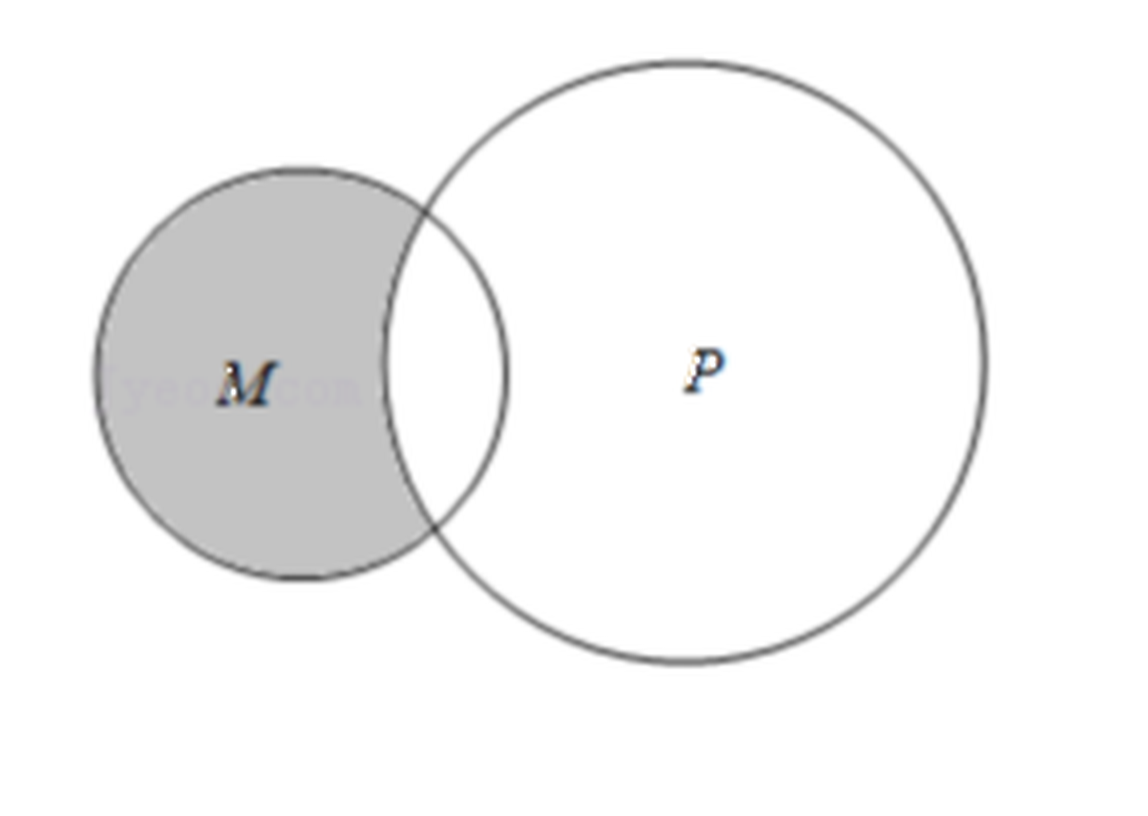
\includegraphics[width=0.36\textwidth]{figures/venn_M_shaded_P.png}
\end{center}

\step{阴影部分表示 $M-P$，所以 $M-(M-P)=M\cap P$. 故选 $B$.}
\solend

\fi

\item 设 $A_1$、$A_2$、$\cdots$、$A_7$ 均是含有 2 个元素的集合，且满足：

$A_i\cap A_{i+1}=\varnothing(i=1,2,3,4,5,6)$，$A_1\cap A_7=\varnothing$. 记 $B=A_1\cup A_2\cup\cdots\cup A_7$，则 $B$ 中元素个数的最小值是\mbox{（\quad）}

\keepwithprev
A. $4$\qquad B. $5$\qquad C. $6$\qquad D. $7$

\ans{$B$}

\ifanswer
\solbegin
\step{$A_1\cap A_7=\varnothing$，$A_i\cap A_{i+1}=\varnothing(i=1,2,3,4,5,6)$，}
\step{所以 $A_1$ 与 $A_2$ 的元素不同，则 $A_1\cup A_2$ 元素个数为 $4$，}
\step{若 $B$ 中元素个数的最小值是 $4$，则只能是 $A_3=A_1=A_5=A_7$，$A_4=A_2=A_6$，}
\step{与 $A_1\cap A_7=\varnothing$ 矛盾，}
\step{若 $A_3$ 从 $A_1$ 中选择 1 个元素，再加入一个新元素，}
\step{这样 $A_1\cup A_2\cup A_3$ 元素个数为 5 个，}
\step{这 5 个元素适当排列，得到 $A_4$、$A_5$、$A_6$、$A_7$，}
\step{例如 $A_1=\{1,2\},A_2=\{3,4\},A_3=\{1,5\}$，}
\step{取 $A_4=\{2,4\},A_5=\{3,5\},A_6=\{1,2\},A_7=\{3,5\}$，符合题意，}
\step{则 $B$ 中元素个数的最小值是 $2+2+1=5$，故选 $B$.}
\solend

\fi

\end{enumerate}

\bigsec{三、解答题}

\begin{enumerate}
\setcounter{enumi}{13}

\item 设 $A=\{x\mid x^2-ax+a^2-19=0\}$，$B=\{x\mid x^2-5x+6=0\}$，$C=\{x\mid x^2+2x-8=0\}$.

\begin{enumerate}[label=(\arabic*)]
\item 若 $A\cap B$ 非空，且 $A\cap C=\varnothing$，求 $a$ 的值；
\item $A\cap B=A\cap C\neq\varnothing$，求 $a$ 的值.
\end{enumerate}

\ifanswer
\solbegin
\stepm{(1)}{由题意，$C=\{-4,2\}$，}
\step{因为 $A\cap B$ 非空且 $A\cap C=\varnothing$，所以 $3\in A$，}
\step{即 $9-3a+a^2-19=0$，解得 $a=-2$ 或 $a=5$，}
\step{当 $a=-2$ 时，$A=\{3,-5\}$，满足题意；}
\step{当 $a=5$ 时，$A=\{2,3\}$，此时 $A\cap C=\{2\}$，不满足题意；}
\step{综上，$a=-2$；}
\stepm{(2)}{因为 $A\cap B=A\cap C\neq\varnothing$，所以 $2\in A$，}
\step{即 $4-2a+a^2-19=0$，解得 $a=-3$ 或 $a=5$，}
\step{当 $a=-3$ 时，$A=\{2,-5\}$，满足题意；}
\step{当 $a=5$ 时，$A=\{2,3\}$，不满足题意，}
\step{故 $a=-3$.}
\solend

\fi

\ansspace[6]

\item 已知 $A=\{x\mid x<-3\text{ 或 }x>1\}$.

\begin{enumerate}[label=(\arabic*)]
\item 若 $B=\{x\mid x<3m+1\text{ 或 }x>m+2\}$，$A\sub B$，求 $m$ 的取值范围.
\item 若 $B=\{x\mid m+2<x<3m+1\}$，$B\sub A$，求 $m$ 的取值范围.
\end{enumerate}

\ifanswer
\solbegin
\stepm{(1)}{当 $3m+1>m+2$，即 $m>\dfrac{1}{2}$ 时，$B=\R$，满足 $A\sub B$；}
\step{当 $3m+1\leqslant m+2$，即 $m\leqslant\dfrac{1}{2}$ 时，要使 $A\sub B$，}
\step{得 $\begin{cases}3m+1\geqslant-3\text{ ①}\\ m+2\leqslant 1\text{ ②}\end{cases}$，解得 $-\dfrac{4}{3}\leqslant m\leqslant-1$.}
\step{综上所述，$m$ 的取值范围为 $\left\{m\mid -\dfrac{4}{3}\leqslant m\leqslant-1\text{ 或 }m>\dfrac{1}{2}\right\}$；}
\stepm{(2)}{当 $B=\varnothing$ 时，则 $3m+1\leqslant m+2$，即 $m\leqslant\dfrac{1}{2}$ 时，满足 $B\sub A$；}
\step{当 $B\neq\varnothing$ 时，且 $B\sub A$，则 $\begin{cases}3m+1>m+2\\ 3m+1\leqslant-3\text{ 或 }m+2\geqslant 1\end{cases}$，所以 $m>\dfrac{1}{2}$.}
\step{综上所述，$m$ 的取值范围为 $\R$.}
\solend

\fi

\ansspace[6]

% 压轴题：其后已无内容，故作答区全用可丢弃胶水（\ansspace*），并在题目前先量一下版面。
\ansneed{7cm}

\item 已知集合 $A$ 为非空集合，定义

$S=\{x\mid x=a+b,a,b\in A\},T=\{x\mid x=|a-b|,a,b\in A\}$.

\begin{enumerate}[label=(\arabic*)]
\item 若集合 $A=\{1,3\}$，直接写出集合 $S$、$T$（无需写计算过程）；
\item 若集合 $A=\{x_1,x_2,x_3,x_4\}$，$x_1<x_2<x_3<x_4$，且 $T=A$，求证：$x_1+x_4=x_2+x_3$；
\item 若集合 $A=\{x\mid 0\leqslant x\leqslant 2021,x\in\N\}$，$S\cap T=\varnothing$. 记 $|A|$ 为集合 $A$ 中元素的个数，求 $|A|$ 的最大值.
\end{enumerate}

\ifanswer
\solbegin
\stepm{(1)}{$S=\{2,4,6\},T=\{0,2\}$；}
\stepm{(2)}{集合 $T$ 中最小的元素为 0，因为 $T=A$，且 $x_1<x_2<x_3<x_4$，所以 $x_1=0$，}
\step{所以集合 $T$ 中元素为 $x_2-x_1=x_2,x_3-x_1=x_3,x_4-x_1=x_4$，}
\step{以及 $x_3-x_2,x_4-x_2,x_4-x_3$ 均属于 $A$，}
% 注：本行原卷印「所以 $x_3$ 即 $x_4-x_2=x_3-x_1$」，「所以 $x_3$ 即 …」语义不完整，
%     疑有漏排（按本段结论应得 $x_4-x_2=x_3$），无法确证原意，本稿照抄原卷、未改。
\step{因为 $x_1=0<x_3-x_2<x_4-x_2<x_4$，所以 $x_3$ 即 $x_4-x_2=x_3-x_1$，}
\step{即 $x_1+x_4=x_2+x_3$；}
\stepm{(3)}{设 $A=\{a_1,a_2,a_3,\cdots,a_k\}$ 满足题意，其中 $a_1<a_2<\cdots<a_k$，}
\step{则 $2a_1<a_1+a_2<\cdots<a_1+a_k<a_2+a_k<a_3+a_k<\cdots<a_{k-1}+a_k<2a_k$，}
\step{所以 $|S\cup T|\leqslant 2k+1$，所以 $3k-1\leqslant 2a_k+1\leqslant 4043(k\in\N^*)$，}
\step{所以 $k\leqslant 1348$，}
\step{实际上当 $A=\{674,675,676,\cdots,2021\}$ 时满足题意，}
\step{证明如下：设 $A=\{m,m+1,m+2,\cdots,2021\},m\in\N$，}
\step{设 $S=\{2m,2m+1,2m+2,\cdots,4042\}$，$T=\{0,1,2,\cdots,2021-m\}$，}
\step{由题意得 $2021-m<2m$，即 $m>673\dfrac{2}{3}$，}
\step{故 $m$ 的最小值是 674，于是当 $m=674$，$A$ 中的元素最多，}
\step{即 $A=\{674,675,676,\cdots,2021\}$ 时满足题意，}
\step{综上所述，集合 $A$ 中元素的个数的最大值是 $1348$.}
\solend

\fi

\ansspace*[9]

\end{enumerate}

\bigsec{附加题}

\begin{enumerate}
\setcounter{enumi}{16}

\item 设 $A$ 是整数集的一个非空子集，对于 $k\in A$，如果 $k-1\notin A$ 且 $k+1\notin A$，那么 $k$ 是 $A$ 的一个“孤立元”。给定 $S=\{1,2,3,4,5,6,7,8\}$，由 $S$ 的 3 个元素构成的所有集合中，不含“孤立元”的集合共有 \blankline[2.4em] 个.

\ifanswer
\solbegin
\step{由题意得，“孤立元”即为在集合中无与之相邻的元素，}
\step{满足条件的集合有 $\{1,2,3\},\{2,3,4\},\{3,4,5\},\{4,5,6\},\{5,6,7\},\{6,7,8\}$，}
\step{共 6 个集合.}
\solend

\fi

\item 已知 $A\cap B=\varnothing$，$M=\{T\mid T\sub A\}$，$P=\{S\mid S\sub B\}$，则 $M\cap P=$ \blankline[4.4em].

\ans{$\{\varnothing\}$}

\item 已知集合 $A=\{x\mid x=m^2-n^2,m,n\in\Z\}$，写出所有满足集合 $A$ 的偶数 \blankline[4.4em].

\ans{$4n,n\in\Z$}

\item 对于给定的正整数 $n(n\geqslant 2)$ 若有限集合 $A=\{a_1,a_2,\cdots,a_n\}\sub M$，且满足

$a_1+a_2+\cdots+a_n=a_1\cdot a_2\cdots a_n$，则称 $A$ 为集合 $M$ 的 $n$ 元“调和子集”，则自然数集 $\N$ 的所有 3 元“调和子集”为 \blankline[3.6em].

\ans{$\{1,2,3\}$}

\end{enumerate}

\end{document}
"
% 紧凑版：xelatex "\def\iscompact{1}% 高一15_七宝中学_抱孩子练习.tex
%   —— 高一上数学「2026-2027 年七宝中学高一上抱孩子练习 9.8」（试卷版/答案版）
% 试卷版：xelatex 高一15_七宝中学_抱孩子练习.tex
% 答案版：xelatex "\def\isanswer{1}\input{高一15_七宝中学_抱孩子练习.tex}"
% 紧凑版：xelatex "\def\iscompact{1}\input{高一15_七宝中学_抱孩子练习.tex}"
%
% 原始材料是微信公众号图文（公众号「魔都数学加油站」），正文为 7 张 PNG 页（1080×1527）。
% 原文本身就是一份**讲评版**——题目下方直接印出【答案】或【解析】。试题文字、答案与解析
% 均照原卷录入，未改内容。卷面上的粉色斜水印「魔都数学加油站」属水印，未录入。
%
% 卷首标题：原卷印作「2026-2027 年七宝中学高一上抱孩子练习 9.8」——「抱孩子练习」四字
% 确系原卷所印（已放大 imgs_B/00.png 卷首核对），句末的「9.8」亦印在同一标题行内，
% 本稿一并照录，未改作「周末作业」；年份区间按全稿惯例排 en dash。
%
% 与原卷的排版差异（均已在 README「说明」中交代）：
%   ① 原文自**第 3 题**起（第 1、2 题未在该文中发布），故本稿题号亦自 3 起；
%   ② 原卷本就印有「一、填空题」「二、选择题」「三、解答题」三节标题，末节另印「附加题」，
%      本稿照原卷分节，只把标题改排成全稿统一的「大节标题」样式；
%   ③ 原卷填空、选择的答案直接印在题目下方，本稿统一改为试卷版隐去、答案版以【答案】或
%      【解析】给出（第 11 题原卷的答案是写在解析末句「故选 B」里的），使两版彻底分离；
%   ④ 原卷的集合符号 $R$、$Z$、$N$ 有正体与粗体两种写法（第 4 题的 $\mathbf{R}$、
%      第 16(3)、17、19、20 题的 $\mathbf{N}$、$\mathbf{Z}$ 为粗体，第 15 题解析的 $B=R$
%      为正体），本稿按全稿惯例统一写作 $\R$、$\Z$、$\N$；
%   ⑤ 原卷用**半角**括号（第 13 题「$\varnothing(i=1,2,3,4,5,6)$」、第 16(1)「(无需写计算过程)」、
%      第 16(2)「$A=\{x_1,x_2,x_3,x_4\}$」、第 20 题「$n(n\geqslant 2)$」），本稿按全稿惯例排全角；
%   ⑥ 原卷未印副标题，本稿按全稿惯例补出副标题「集合与常用逻辑用语」；
%   ⑦ 第 18、20 题的 $\subseteq$（带下划线，真包含写作 $\subset$ 与之形近）已逐处放大比对确认，
%      第 18 题的答案 $\{\varnothing\}$ 亦与 $\subseteq$ 口径相符（若为真包含则答案应为 $\varnothing$）。
%
% 原卷存疑两处（均已放大到能看清字形后核对，无法确证原意，本稿照抄原卷、未改）：
%   ① 第 10 题【解析】末句原卷印「所以 $1-k^2\neq 0$，即 $k\neq\pm 1$」——按此式，当 $k=1$
%      时两方程为同一直线、有无穷多解，$A\cap B\neq\varnothing$ 仍成立，故 $A\cap B\neq\varnothing$
%      当且仅当 $k\neq -1$；原卷结论与题设不合，疑为原卷笔误，但无法确证原意，本稿照抄原卷；
%   ② 第 16(2)【解析】原卷印「因为 $x_1=0<x_3-x_2<x_4-x_2<x_4$，所以 $x_3$ 即 $x_4-x_2=x_3-x_1$，」
%      ——「所以 $x_3$ 即 …」一句语义不完整，疑有漏排（按本段结论应得 $x_4-x_2=x_3$），
%      无法确证原意，本稿照抄原卷。

\documentclass[a4paper,11pt]{article}
\usepackage{common}

\begin{document}

\examtitlest[3]{2026--2027 年七宝中学高一上抱孩子练习 9.8}{集合与常用逻辑用语}

\bigsec{一、填空题}

\begin{enumerate}
\setcounter{enumi}{2}

\item 方程 $\sqrt{x+2}=-x$ 的解的集合为 \blankline[4.4em].

\ifanswer
\solbegin
\step{因为 $\sqrt{x+2}=-x$，所以 $\begin{cases}x\leqslant 0\\ x+2=x^2\end{cases}$，解得 $x=-1$，}
\step{所以方程 $\sqrt{x+2}=-x$ 的解的集合为 $\{-1\}$.}
\solend

\fi

\item 若 $A=\{x\mid a-4<x\leqslant a+4\}$，$B=\{x\mid x>5\text{ 或 }x<-1\}$，且 $A\cup B=\R$，则实数 $a$ 的取值范围是 \blankline[3.6em].

\ans{$[1,3)$}

\item 设集合 $A=\{x\mid x=2n+1,n\in\N\}$，$B=\{x\mid x=3n,n\in\N\}$，则 $A\cap B=$ \blankline[4.4em].

\ans{$\{x\mid x=6n+3,n\in\N\}$}

\item 已知集合 $A=\{1,2\}$，集合 $B=\{x\mid ax=6\}$，若 $A\cup B=A$，则 $a$ 的所有取值构成的集合为 \blankline[4.4em].

\ifanswer
\solbegin
\step{因为 $A\cup B=A$，所以 $B\sub A$，}
\step{当 $a=0$ 时，$B=\varnothing$，满足 $B\sub A$；}
\step{当 $a\neq 0$ 时，$B=\left\{\dfrac{6}{a}\right\}$，则 $\dfrac{6}{a}=1$ 或 $\dfrac{6}{a}=2$，解得 $a=6$ 或 $a=3$，}
\step{综上所述，$a$ 的所有取值构成的集合为 $\{0,3,6\}$.}
\solend

\fi

\item 设 $U=\{2,4,a^2-a+1\}$，$A=\{2,|a+1|\}$，$\overline{A}=\{7\}$，则 $a=$ \blankline[2.4em].

\ans{$3$}

\item 已知集合 $A=\{x\mid x^2-px-q=0\}$，$B=\{x\mid x^2+qx-p=0\}$，且 $A\cap B=\{1\}$，则 $A\cup B=$ \blankline[4.4em].

\ans{$\{0,-1,1\}$}

\item 定义集合运算：$A\odot B=\{z\mid z=xy(x+y),x\in A,y\in B\}$，若 $A=\{1,2\},B=\{3,4\}$，则 $A\odot B$ 的所有元素之和是 \blankline[3.6em].

\ans{$110$}

\item 已知集合 $A=\{(x,y)\mid kx+y=k+1\}$，$B=\{(x,y)\mid x+ky=2k\}$，其中 $k$ 为实数，$A\cap B\neq\varnothing$，则 $k$ 的取值范围是 \blankline[4.4em].

\ifanswer
\solbegin
\step{因为 $A\cap B\neq\varnothing$，所以方程组 $\begin{cases}kx+y=k+1\\ x+ky=2k\end{cases}$ 有解，消 $y$ 得 $(1-k^2)x=k-k^2$，}
% 注：末句原卷印「所以 $1-k^2\neq 0$，即 $k\neq\pm 1$」。按此式，$k=1$ 时两方程为同一直线、
%     有无穷多解，$A\cap B\neq\varnothing$ 仍成立，故结论应为 $k\neq -1$。疑为原卷笔误，
%     但无法确证原意，本稿照抄原卷、未改（详见文件头「原卷存疑」①）。
\step{所以 $1-k^2\neq 0$，即 $k\neq\pm 1$.}
\solend

\fi

\end{enumerate}

\bigsec{二、选择题}

\begin{enumerate}
\setcounter{enumi}{10}

\item 给出关系式：①$0\in\varnothing$；②$\varnothing=\{0\}$；③$\{a,b\}=\{b,a\}$；④$\{y\mid y=x^2-2\}=\{(x,y)\mid y=x^2-2\}$，其中正确的关系式的个数是\mbox{（\quad）}

\keepwithprev
A. $0$\qquad B. $1$\qquad C. $2$\qquad D. $3$

\ans{$B$}

\ifanswer
\solbegin
\step{在①中，$\varnothing$ 表示空集，$0\notin\varnothing$，故①错误；在②中，$\varnothing\sub\{0\}$，故②错误；}
\step{在③中，$\{a,b\}=\{b,a\}$，故③正确；}
\step{在④中，因为，$\{y\mid y=x^2-2\}$ 和 $\{(x,y)\mid y=x^2-2\}$ 的代表元素不同，}
\step{所以 $\{y\mid y=x^2-2\}\neq\{(x,y)\mid y=x^2-2\}$，故④错误.}
\step{故正确的是③，故选 $B$.}
\solend

\fi

\item 设集合 $M$、$P\neq\varnothing$，定义集合 $M-P=\{x\mid x\in M,x\notin P\}$，则集合 $M-(M-P)$ 是\mbox{（\quad）}

\keepwithprev
A. $P$\qquad B. $M$\qquad C. $M\cup P$\qquad D. $M\cap P$

\ans{$B$}

\ifanswer
\solbegin
\step{$M-(M-P)=\{x\mid x\in M,\text{ 且 }x\notin(M-P)\}$，}
\step{用 venn 图表示集合 $M$、$P$ 的关系如图：}

\begin{center}
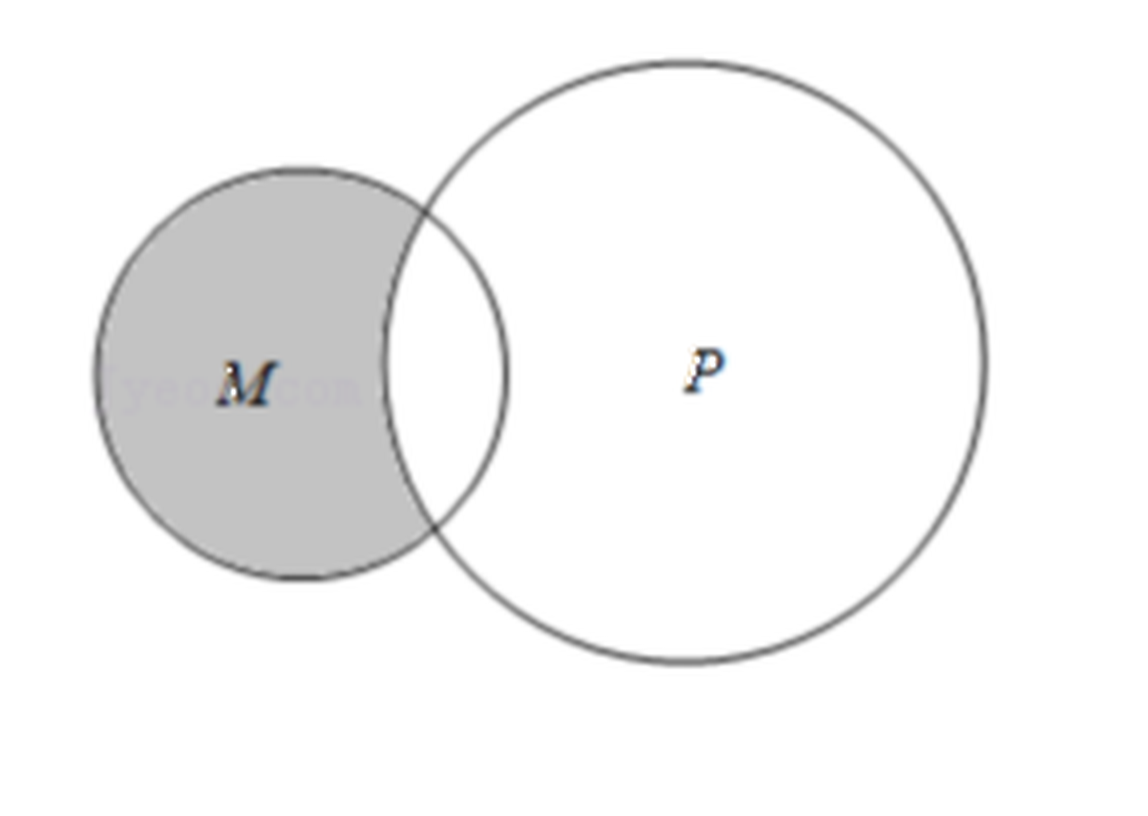
\includegraphics[width=0.36\textwidth]{figures/venn_M_shaded_P.png}
\end{center}

\step{阴影部分表示 $M-P$，所以 $M-(M-P)=M\cap P$. 故选 $B$.}
\solend

\fi

\item 设 $A_1$、$A_2$、$\cdots$、$A_7$ 均是含有 2 个元素的集合，且满足：

$A_i\cap A_{i+1}=\varnothing(i=1,2,3,4,5,6)$，$A_1\cap A_7=\varnothing$. 记 $B=A_1\cup A_2\cup\cdots\cup A_7$，则 $B$ 中元素个数的最小值是\mbox{（\quad）}

\keepwithprev
A. $4$\qquad B. $5$\qquad C. $6$\qquad D. $7$

\ans{$B$}

\ifanswer
\solbegin
\step{$A_1\cap A_7=\varnothing$，$A_i\cap A_{i+1}=\varnothing(i=1,2,3,4,5,6)$，}
\step{所以 $A_1$ 与 $A_2$ 的元素不同，则 $A_1\cup A_2$ 元素个数为 $4$，}
\step{若 $B$ 中元素个数的最小值是 $4$，则只能是 $A_3=A_1=A_5=A_7$，$A_4=A_2=A_6$，}
\step{与 $A_1\cap A_7=\varnothing$ 矛盾，}
\step{若 $A_3$ 从 $A_1$ 中选择 1 个元素，再加入一个新元素，}
\step{这样 $A_1\cup A_2\cup A_3$ 元素个数为 5 个，}
\step{这 5 个元素适当排列，得到 $A_4$、$A_5$、$A_6$、$A_7$，}
\step{例如 $A_1=\{1,2\},A_2=\{3,4\},A_3=\{1,5\}$，}
\step{取 $A_4=\{2,4\},A_5=\{3,5\},A_6=\{1,2\},A_7=\{3,5\}$，符合题意，}
\step{则 $B$ 中元素个数的最小值是 $2+2+1=5$，故选 $B$.}
\solend

\fi

\end{enumerate}

\bigsec{三、解答题}

\begin{enumerate}
\setcounter{enumi}{13}

\item 设 $A=\{x\mid x^2-ax+a^2-19=0\}$，$B=\{x\mid x^2-5x+6=0\}$，$C=\{x\mid x^2+2x-8=0\}$.

\begin{enumerate}[label=(\arabic*)]
\item 若 $A\cap B$ 非空，且 $A\cap C=\varnothing$，求 $a$ 的值；
\item $A\cap B=A\cap C\neq\varnothing$，求 $a$ 的值.
\end{enumerate}

\ifanswer
\solbegin
\stepm{(1)}{由题意，$C=\{-4,2\}$，}
\step{因为 $A\cap B$ 非空且 $A\cap C=\varnothing$，所以 $3\in A$，}
\step{即 $9-3a+a^2-19=0$，解得 $a=-2$ 或 $a=5$，}
\step{当 $a=-2$ 时，$A=\{3,-5\}$，满足题意；}
\step{当 $a=5$ 时，$A=\{2,3\}$，此时 $A\cap C=\{2\}$，不满足题意；}
\step{综上，$a=-2$；}
\stepm{(2)}{因为 $A\cap B=A\cap C\neq\varnothing$，所以 $2\in A$，}
\step{即 $4-2a+a^2-19=0$，解得 $a=-3$ 或 $a=5$，}
\step{当 $a=-3$ 时，$A=\{2,-5\}$，满足题意；}
\step{当 $a=5$ 时，$A=\{2,3\}$，不满足题意，}
\step{故 $a=-3$.}
\solend

\fi

\ansspace[6]

\item 已知 $A=\{x\mid x<-3\text{ 或 }x>1\}$.

\begin{enumerate}[label=(\arabic*)]
\item 若 $B=\{x\mid x<3m+1\text{ 或 }x>m+2\}$，$A\sub B$，求 $m$ 的取值范围.
\item 若 $B=\{x\mid m+2<x<3m+1\}$，$B\sub A$，求 $m$ 的取值范围.
\end{enumerate}

\ifanswer
\solbegin
\stepm{(1)}{当 $3m+1>m+2$，即 $m>\dfrac{1}{2}$ 时，$B=\R$，满足 $A\sub B$；}
\step{当 $3m+1\leqslant m+2$，即 $m\leqslant\dfrac{1}{2}$ 时，要使 $A\sub B$，}
\step{得 $\begin{cases}3m+1\geqslant-3\text{ ①}\\ m+2\leqslant 1\text{ ②}\end{cases}$，解得 $-\dfrac{4}{3}\leqslant m\leqslant-1$.}
\step{综上所述，$m$ 的取值范围为 $\left\{m\mid -\dfrac{4}{3}\leqslant m\leqslant-1\text{ 或 }m>\dfrac{1}{2}\right\}$；}
\stepm{(2)}{当 $B=\varnothing$ 时，则 $3m+1\leqslant m+2$，即 $m\leqslant\dfrac{1}{2}$ 时，满足 $B\sub A$；}
\step{当 $B\neq\varnothing$ 时，且 $B\sub A$，则 $\begin{cases}3m+1>m+2\\ 3m+1\leqslant-3\text{ 或 }m+2\geqslant 1\end{cases}$，所以 $m>\dfrac{1}{2}$.}
\step{综上所述，$m$ 的取值范围为 $\R$.}
\solend

\fi

\ansspace[6]

% 压轴题：其后已无内容，故作答区全用可丢弃胶水（\ansspace*），并在题目前先量一下版面。
\ansneed{7cm}

\item 已知集合 $A$ 为非空集合，定义

$S=\{x\mid x=a+b,a,b\in A\},T=\{x\mid x=|a-b|,a,b\in A\}$.

\begin{enumerate}[label=(\arabic*)]
\item 若集合 $A=\{1,3\}$，直接写出集合 $S$、$T$（无需写计算过程）；
\item 若集合 $A=\{x_1,x_2,x_3,x_4\}$，$x_1<x_2<x_3<x_4$，且 $T=A$，求证：$x_1+x_4=x_2+x_3$；
\item 若集合 $A=\{x\mid 0\leqslant x\leqslant 2021,x\in\N\}$，$S\cap T=\varnothing$. 记 $|A|$ 为集合 $A$ 中元素的个数，求 $|A|$ 的最大值.
\end{enumerate}

\ifanswer
\solbegin
\stepm{(1)}{$S=\{2,4,6\},T=\{0,2\}$；}
\stepm{(2)}{集合 $T$ 中最小的元素为 0，因为 $T=A$，且 $x_1<x_2<x_3<x_4$，所以 $x_1=0$，}
\step{所以集合 $T$ 中元素为 $x_2-x_1=x_2,x_3-x_1=x_3,x_4-x_1=x_4$，}
\step{以及 $x_3-x_2,x_4-x_2,x_4-x_3$ 均属于 $A$，}
% 注：本行原卷印「所以 $x_3$ 即 $x_4-x_2=x_3-x_1$」，「所以 $x_3$ 即 …」语义不完整，
%     疑有漏排（按本段结论应得 $x_4-x_2=x_3$），无法确证原意，本稿照抄原卷、未改。
\step{因为 $x_1=0<x_3-x_2<x_4-x_2<x_4$，所以 $x_3$ 即 $x_4-x_2=x_3-x_1$，}
\step{即 $x_1+x_4=x_2+x_3$；}
\stepm{(3)}{设 $A=\{a_1,a_2,a_3,\cdots,a_k\}$ 满足题意，其中 $a_1<a_2<\cdots<a_k$，}
\step{则 $2a_1<a_1+a_2<\cdots<a_1+a_k<a_2+a_k<a_3+a_k<\cdots<a_{k-1}+a_k<2a_k$，}
\step{所以 $|S\cup T|\leqslant 2k+1$，所以 $3k-1\leqslant 2a_k+1\leqslant 4043(k\in\N^*)$，}
\step{所以 $k\leqslant 1348$，}
\step{实际上当 $A=\{674,675,676,\cdots,2021\}$ 时满足题意，}
\step{证明如下：设 $A=\{m,m+1,m+2,\cdots,2021\},m\in\N$，}
\step{设 $S=\{2m,2m+1,2m+2,\cdots,4042\}$，$T=\{0,1,2,\cdots,2021-m\}$，}
\step{由题意得 $2021-m<2m$，即 $m>673\dfrac{2}{3}$，}
\step{故 $m$ 的最小值是 674，于是当 $m=674$，$A$ 中的元素最多，}
\step{即 $A=\{674,675,676,\cdots,2021\}$ 时满足题意，}
\step{综上所述，集合 $A$ 中元素的个数的最大值是 $1348$.}
\solend

\fi

\ansspace*[9]

\end{enumerate}

\bigsec{附加题}

\begin{enumerate}
\setcounter{enumi}{16}

\item 设 $A$ 是整数集的一个非空子集，对于 $k\in A$，如果 $k-1\notin A$ 且 $k+1\notin A$，那么 $k$ 是 $A$ 的一个“孤立元”。给定 $S=\{1,2,3,4,5,6,7,8\}$，由 $S$ 的 3 个元素构成的所有集合中，不含“孤立元”的集合共有 \blankline[2.4em] 个.

\ifanswer
\solbegin
\step{由题意得，“孤立元”即为在集合中无与之相邻的元素，}
\step{满足条件的集合有 $\{1,2,3\},\{2,3,4\},\{3,4,5\},\{4,5,6\},\{5,6,7\},\{6,7,8\}$，}
\step{共 6 个集合.}
\solend

\fi

\item 已知 $A\cap B=\varnothing$，$M=\{T\mid T\sub A\}$，$P=\{S\mid S\sub B\}$，则 $M\cap P=$ \blankline[4.4em].

\ans{$\{\varnothing\}$}

\item 已知集合 $A=\{x\mid x=m^2-n^2,m,n\in\Z\}$，写出所有满足集合 $A$ 的偶数 \blankline[4.4em].

\ans{$4n,n\in\Z$}

\item 对于给定的正整数 $n(n\geqslant 2)$ 若有限集合 $A=\{a_1,a_2,\cdots,a_n\}\sub M$，且满足

$a_1+a_2+\cdots+a_n=a_1\cdot a_2\cdots a_n$，则称 $A$ 为集合 $M$ 的 $n$ 元“调和子集”，则自然数集 $\N$ 的所有 3 元“调和子集”为 \blankline[3.6em].

\ans{$\{1,2,3\}$}

\end{enumerate}

\end{document}
"
%
% 原始材料是微信公众号图文（公众号「魔都数学加油站」），正文为 7 张 PNG 页（1080×1527）。
% 原文本身就是一份**讲评版**——题目下方直接印出【答案】或【解析】。试题文字、答案与解析
% 均照原卷录入，未改内容。卷面上的粉色斜水印「魔都数学加油站」属水印，未录入。
%
% 卷首标题：原卷印作「2026-2027 年七宝中学高一上抱孩子练习 9.8」——「抱孩子练习」四字
% 确系原卷所印（已放大 imgs_B/00.png 卷首核对），句末的「9.8」亦印在同一标题行内，
% 本稿一并照录，未改作「周末作业」；年份区间按全稿惯例排 en dash。
%
% 与原卷的排版差异（均已在 README「说明」中交代）：
%   ① 原文自**第 3 题**起（第 1、2 题未在该文中发布），故本稿题号亦自 3 起；
%   ② 原卷本就印有「一、填空题」「二、选择题」「三、解答题」三节标题，末节另印「附加题」，
%      本稿照原卷分节，只把标题改排成全稿统一的「大节标题」样式；
%   ③ 原卷填空、选择的答案直接印在题目下方，本稿统一改为试卷版隐去、答案版以【答案】或
%      【解析】给出（第 11 题原卷的答案是写在解析末句「故选 B」里的），使两版彻底分离；
%   ④ 原卷的集合符号 $R$、$Z$、$N$ 有正体与粗体两种写法（第 4 题的 $\mathbf{R}$、
%      第 16(3)、17、19、20 题的 $\mathbf{N}$、$\mathbf{Z}$ 为粗体，第 15 题解析的 $B=R$
%      为正体），本稿按全稿惯例统一写作 $\R$、$\Z$、$\N$；
%   ⑤ 原卷用**半角**括号（第 13 题「$\varnothing(i=1,2,3,4,5,6)$」、第 16(1)「(无需写计算过程)」、
%      第 16(2)「$A=\{x_1,x_2,x_3,x_4\}$」、第 20 题「$n(n\geqslant 2)$」），本稿按全稿惯例排全角；
%   ⑥ 原卷未印副标题，本稿按全稿惯例补出副标题「集合与常用逻辑用语」；
%   ⑦ 第 18、20 题的 $\subseteq$（带下划线，真包含写作 $\subset$ 与之形近）已逐处放大比对确认，
%      第 18 题的答案 $\{\varnothing\}$ 亦与 $\subseteq$ 口径相符（若为真包含则答案应为 $\varnothing$）。
%
% 原卷存疑两处（均已放大到能看清字形后核对，无法确证原意，本稿照抄原卷、未改）：
%   ① 第 10 题【解析】末句原卷印「所以 $1-k^2\neq 0$，即 $k\neq\pm 1$」——按此式，当 $k=1$
%      时两方程为同一直线、有无穷多解，$A\cap B\neq\varnothing$ 仍成立，故 $A\cap B\neq\varnothing$
%      当且仅当 $k\neq -1$；原卷结论与题设不合，疑为原卷笔误，但无法确证原意，本稿照抄原卷；
%   ② 第 16(2)【解析】原卷印「因为 $x_1=0<x_3-x_2<x_4-x_2<x_4$，所以 $x_3$ 即 $x_4-x_2=x_3-x_1$，」
%      ——「所以 $x_3$ 即 …」一句语义不完整，疑有漏排（按本段结论应得 $x_4-x_2=x_3$），
%      无法确证原意，本稿照抄原卷。

\documentclass[a4paper,11pt]{article}
\usepackage{common}

\begin{document}

\examtitlest[3]{2026--2027 年七宝中学高一上抱孩子练习 9.8}{集合与常用逻辑用语}

\bigsec{一、填空题}

\begin{enumerate}
\setcounter{enumi}{2}

\item 方程 $\sqrt{x+2}=-x$ 的解的集合为 \blankline[4.4em].

\ifanswer
\solbegin
\step{因为 $\sqrt{x+2}=-x$，所以 $\begin{cases}x\leqslant 0\\ x+2=x^2\end{cases}$，解得 $x=-1$，}
\step{所以方程 $\sqrt{x+2}=-x$ 的解的集合为 $\{-1\}$.}
\solend

\fi

\item 若 $A=\{x\mid a-4<x\leqslant a+4\}$，$B=\{x\mid x>5\text{ 或 }x<-1\}$，且 $A\cup B=\R$，则实数 $a$ 的取值范围是 \blankline[3.6em].

\ans{$[1,3)$}

\item 设集合 $A=\{x\mid x=2n+1,n\in\N\}$，$B=\{x\mid x=3n,n\in\N\}$，则 $A\cap B=$ \blankline[4.4em].

\ans{$\{x\mid x=6n+3,n\in\N\}$}

\item 已知集合 $A=\{1,2\}$，集合 $B=\{x\mid ax=6\}$，若 $A\cup B=A$，则 $a$ 的所有取值构成的集合为 \blankline[4.4em].

\ifanswer
\solbegin
\step{因为 $A\cup B=A$，所以 $B\sub A$，}
\step{当 $a=0$ 时，$B=\varnothing$，满足 $B\sub A$；}
\step{当 $a\neq 0$ 时，$B=\left\{\dfrac{6}{a}\right\}$，则 $\dfrac{6}{a}=1$ 或 $\dfrac{6}{a}=2$，解得 $a=6$ 或 $a=3$，}
\step{综上所述，$a$ 的所有取值构成的集合为 $\{0,3,6\}$.}
\solend

\fi

\item 设 $U=\{2,4,a^2-a+1\}$，$A=\{2,|a+1|\}$，$\overline{A}=\{7\}$，则 $a=$ \blankline[2.4em].

\ans{$3$}

\item 已知集合 $A=\{x\mid x^2-px-q=0\}$，$B=\{x\mid x^2+qx-p=0\}$，且 $A\cap B=\{1\}$，则 $A\cup B=$ \blankline[4.4em].

\ans{$\{0,-1,1\}$}

\item 定义集合运算：$A\odot B=\{z\mid z=xy(x+y),x\in A,y\in B\}$，若 $A=\{1,2\},B=\{3,4\}$，则 $A\odot B$ 的所有元素之和是 \blankline[3.6em].

\ans{$110$}

\item 已知集合 $A=\{(x,y)\mid kx+y=k+1\}$，$B=\{(x,y)\mid x+ky=2k\}$，其中 $k$ 为实数，$A\cap B\neq\varnothing$，则 $k$ 的取值范围是 \blankline[4.4em].

\ifanswer
\solbegin
\step{因为 $A\cap B\neq\varnothing$，所以方程组 $\begin{cases}kx+y=k+1\\ x+ky=2k\end{cases}$ 有解，消 $y$ 得 $(1-k^2)x=k-k^2$，}
% 注：末句原卷印「所以 $1-k^2\neq 0$，即 $k\neq\pm 1$」。按此式，$k=1$ 时两方程为同一直线、
%     有无穷多解，$A\cap B\neq\varnothing$ 仍成立，故结论应为 $k\neq -1$。疑为原卷笔误，
%     但无法确证原意，本稿照抄原卷、未改（详见文件头「原卷存疑」①）。
\step{所以 $1-k^2\neq 0$，即 $k\neq\pm 1$.}
\solend

\fi

\end{enumerate}

\bigsec{二、选择题}

\begin{enumerate}
\setcounter{enumi}{10}

\item 给出关系式：①$0\in\varnothing$；②$\varnothing=\{0\}$；③$\{a,b\}=\{b,a\}$；④$\{y\mid y=x^2-2\}=\{(x,y)\mid y=x^2-2\}$，其中正确的关系式的个数是\mbox{（\quad）}

\keepwithprev
A. $0$\qquad B. $1$\qquad C. $2$\qquad D. $3$

\ans{$B$}

\ifanswer
\solbegin
\step{在①中，$\varnothing$ 表示空集，$0\notin\varnothing$，故①错误；在②中，$\varnothing\sub\{0\}$，故②错误；}
\step{在③中，$\{a,b\}=\{b,a\}$，故③正确；}
\step{在④中，因为，$\{y\mid y=x^2-2\}$ 和 $\{(x,y)\mid y=x^2-2\}$ 的代表元素不同，}
\step{所以 $\{y\mid y=x^2-2\}\neq\{(x,y)\mid y=x^2-2\}$，故④错误.}
\step{故正确的是③，故选 $B$.}
\solend

\fi

\item 设集合 $M$、$P\neq\varnothing$，定义集合 $M-P=\{x\mid x\in M,x\notin P\}$，则集合 $M-(M-P)$ 是\mbox{（\quad）}

\keepwithprev
A. $P$\qquad B. $M$\qquad C. $M\cup P$\qquad D. $M\cap P$

\ans{$B$}

\ifanswer
\solbegin
\step{$M-(M-P)=\{x\mid x\in M,\text{ 且 }x\notin(M-P)\}$，}
\step{用 venn 图表示集合 $M$、$P$ 的关系如图：}

\begin{center}
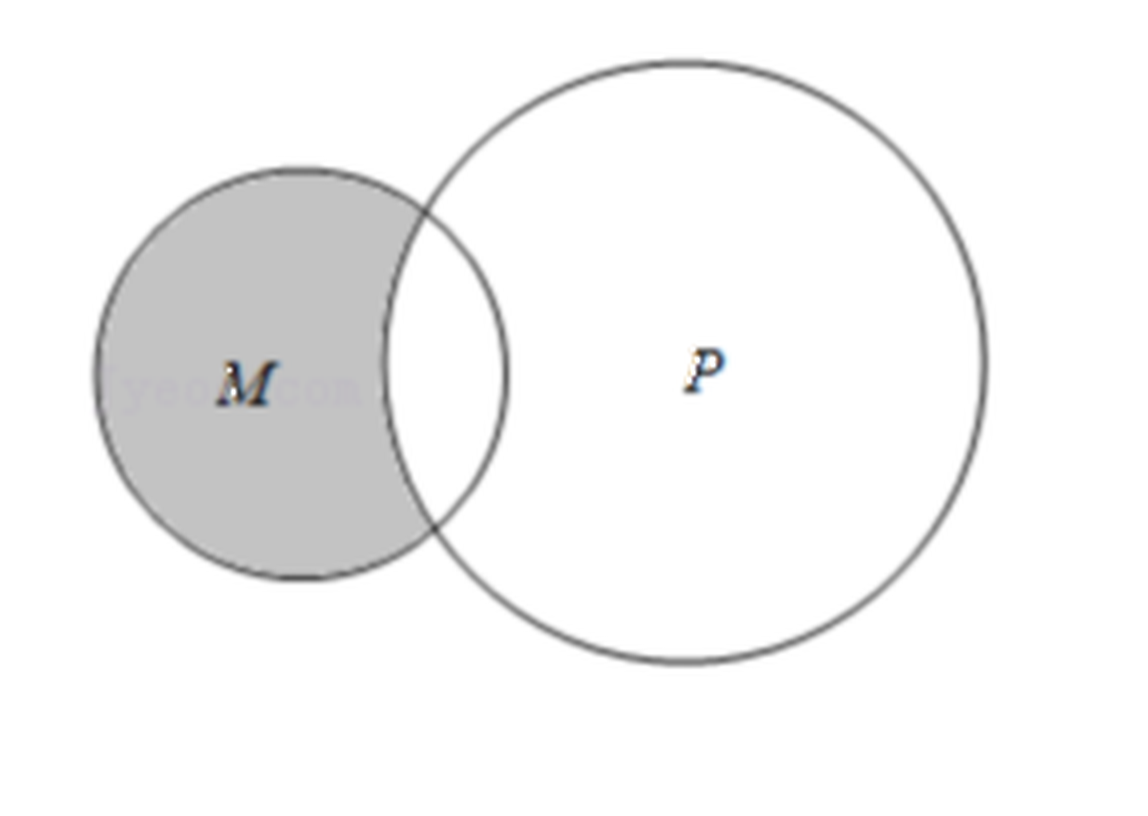
\includegraphics[width=0.36\textwidth]{figures/venn_M_shaded_P.png}
\end{center}

\step{阴影部分表示 $M-P$，所以 $M-(M-P)=M\cap P$. 故选 $B$.}
\solend

\fi

\item 设 $A_1$、$A_2$、$\cdots$、$A_7$ 均是含有 2 个元素的集合，且满足：

$A_i\cap A_{i+1}=\varnothing(i=1,2,3,4,5,6)$，$A_1\cap A_7=\varnothing$. 记 $B=A_1\cup A_2\cup\cdots\cup A_7$，则 $B$ 中元素个数的最小值是\mbox{（\quad）}

\keepwithprev
A. $4$\qquad B. $5$\qquad C. $6$\qquad D. $7$

\ans{$B$}

\ifanswer
\solbegin
\step{$A_1\cap A_7=\varnothing$，$A_i\cap A_{i+1}=\varnothing(i=1,2,3,4,5,6)$，}
\step{所以 $A_1$ 与 $A_2$ 的元素不同，则 $A_1\cup A_2$ 元素个数为 $4$，}
\step{若 $B$ 中元素个数的最小值是 $4$，则只能是 $A_3=A_1=A_5=A_7$，$A_4=A_2=A_6$，}
\step{与 $A_1\cap A_7=\varnothing$ 矛盾，}
\step{若 $A_3$ 从 $A_1$ 中选择 1 个元素，再加入一个新元素，}
\step{这样 $A_1\cup A_2\cup A_3$ 元素个数为 5 个，}
\step{这 5 个元素适当排列，得到 $A_4$、$A_5$、$A_6$、$A_7$，}
\step{例如 $A_1=\{1,2\},A_2=\{3,4\},A_3=\{1,5\}$，}
\step{取 $A_4=\{2,4\},A_5=\{3,5\},A_6=\{1,2\},A_7=\{3,5\}$，符合题意，}
\step{则 $B$ 中元素个数的最小值是 $2+2+1=5$，故选 $B$.}
\solend

\fi

\end{enumerate}

\bigsec{三、解答题}

\begin{enumerate}
\setcounter{enumi}{13}

\item 设 $A=\{x\mid x^2-ax+a^2-19=0\}$，$B=\{x\mid x^2-5x+6=0\}$，$C=\{x\mid x^2+2x-8=0\}$.

\begin{enumerate}[label=(\arabic*)]
\item 若 $A\cap B$ 非空，且 $A\cap C=\varnothing$，求 $a$ 的值；
\item $A\cap B=A\cap C\neq\varnothing$，求 $a$ 的值.
\end{enumerate}

\ifanswer
\solbegin
\stepm{(1)}{由题意，$C=\{-4,2\}$，}
\step{因为 $A\cap B$ 非空且 $A\cap C=\varnothing$，所以 $3\in A$，}
\step{即 $9-3a+a^2-19=0$，解得 $a=-2$ 或 $a=5$，}
\step{当 $a=-2$ 时，$A=\{3,-5\}$，满足题意；}
\step{当 $a=5$ 时，$A=\{2,3\}$，此时 $A\cap C=\{2\}$，不满足题意；}
\step{综上，$a=-2$；}
\stepm{(2)}{因为 $A\cap B=A\cap C\neq\varnothing$，所以 $2\in A$，}
\step{即 $4-2a+a^2-19=0$，解得 $a=-3$ 或 $a=5$，}
\step{当 $a=-3$ 时，$A=\{2,-5\}$，满足题意；}
\step{当 $a=5$ 时，$A=\{2,3\}$，不满足题意，}
\step{故 $a=-3$.}
\solend

\fi

\ansspace[6]

\item 已知 $A=\{x\mid x<-3\text{ 或 }x>1\}$.

\begin{enumerate}[label=(\arabic*)]
\item 若 $B=\{x\mid x<3m+1\text{ 或 }x>m+2\}$，$A\sub B$，求 $m$ 的取值范围.
\item 若 $B=\{x\mid m+2<x<3m+1\}$，$B\sub A$，求 $m$ 的取值范围.
\end{enumerate}

\ifanswer
\solbegin
\stepm{(1)}{当 $3m+1>m+2$，即 $m>\dfrac{1}{2}$ 时，$B=\R$，满足 $A\sub B$；}
\step{当 $3m+1\leqslant m+2$，即 $m\leqslant\dfrac{1}{2}$ 时，要使 $A\sub B$，}
\step{得 $\begin{cases}3m+1\geqslant-3\text{ ①}\\ m+2\leqslant 1\text{ ②}\end{cases}$，解得 $-\dfrac{4}{3}\leqslant m\leqslant-1$.}
\step{综上所述，$m$ 的取值范围为 $\left\{m\mid -\dfrac{4}{3}\leqslant m\leqslant-1\text{ 或 }m>\dfrac{1}{2}\right\}$；}
\stepm{(2)}{当 $B=\varnothing$ 时，则 $3m+1\leqslant m+2$，即 $m\leqslant\dfrac{1}{2}$ 时，满足 $B\sub A$；}
\step{当 $B\neq\varnothing$ 时，且 $B\sub A$，则 $\begin{cases}3m+1>m+2\\ 3m+1\leqslant-3\text{ 或 }m+2\geqslant 1\end{cases}$，所以 $m>\dfrac{1}{2}$.}
\step{综上所述，$m$ 的取值范围为 $\R$.}
\solend

\fi

\ansspace[6]

% 压轴题：其后已无内容，故作答区全用可丢弃胶水（\ansspace*），并在题目前先量一下版面。
\ansneed{7cm}

\item 已知集合 $A$ 为非空集合，定义

$S=\{x\mid x=a+b,a,b\in A\},T=\{x\mid x=|a-b|,a,b\in A\}$.

\begin{enumerate}[label=(\arabic*)]
\item 若集合 $A=\{1,3\}$，直接写出集合 $S$、$T$（无需写计算过程）；
\item 若集合 $A=\{x_1,x_2,x_3,x_4\}$，$x_1<x_2<x_3<x_4$，且 $T=A$，求证：$x_1+x_4=x_2+x_3$；
\item 若集合 $A=\{x\mid 0\leqslant x\leqslant 2021,x\in\N\}$，$S\cap T=\varnothing$. 记 $|A|$ 为集合 $A$ 中元素的个数，求 $|A|$ 的最大值.
\end{enumerate}

\ifanswer
\solbegin
\stepm{(1)}{$S=\{2,4,6\},T=\{0,2\}$；}
\stepm{(2)}{集合 $T$ 中最小的元素为 0，因为 $T=A$，且 $x_1<x_2<x_3<x_4$，所以 $x_1=0$，}
\step{所以集合 $T$ 中元素为 $x_2-x_1=x_2,x_3-x_1=x_3,x_4-x_1=x_4$，}
\step{以及 $x_3-x_2,x_4-x_2,x_4-x_3$ 均属于 $A$，}
% 注：本行原卷印「所以 $x_3$ 即 $x_4-x_2=x_3-x_1$」，「所以 $x_3$ 即 …」语义不完整，
%     疑有漏排（按本段结论应得 $x_4-x_2=x_3$），无法确证原意，本稿照抄原卷、未改。
\step{因为 $x_1=0<x_3-x_2<x_4-x_2<x_4$，所以 $x_3$ 即 $x_4-x_2=x_3-x_1$，}
\step{即 $x_1+x_4=x_2+x_3$；}
\stepm{(3)}{设 $A=\{a_1,a_2,a_3,\cdots,a_k\}$ 满足题意，其中 $a_1<a_2<\cdots<a_k$，}
\step{则 $2a_1<a_1+a_2<\cdots<a_1+a_k<a_2+a_k<a_3+a_k<\cdots<a_{k-1}+a_k<2a_k$，}
\step{所以 $|S\cup T|\leqslant 2k+1$，所以 $3k-1\leqslant 2a_k+1\leqslant 4043(k\in\N^*)$，}
\step{所以 $k\leqslant 1348$，}
\step{实际上当 $A=\{674,675,676,\cdots,2021\}$ 时满足题意，}
\step{证明如下：设 $A=\{m,m+1,m+2,\cdots,2021\},m\in\N$，}
\step{设 $S=\{2m,2m+1,2m+2,\cdots,4042\}$，$T=\{0,1,2,\cdots,2021-m\}$，}
\step{由题意得 $2021-m<2m$，即 $m>673\dfrac{2}{3}$，}
\step{故 $m$ 的最小值是 674，于是当 $m=674$，$A$ 中的元素最多，}
\step{即 $A=\{674,675,676,\cdots,2021\}$ 时满足题意，}
\step{综上所述，集合 $A$ 中元素的个数的最大值是 $1348$.}
\solend

\fi

\ansspace*[9]

\end{enumerate}

\bigsec{附加题}

\begin{enumerate}
\setcounter{enumi}{16}

\item 设 $A$ 是整数集的一个非空子集，对于 $k\in A$，如果 $k-1\notin A$ 且 $k+1\notin A$，那么 $k$ 是 $A$ 的一个“孤立元”。给定 $S=\{1,2,3,4,5,6,7,8\}$，由 $S$ 的 3 个元素构成的所有集合中，不含“孤立元”的集合共有 \blankline[2.4em] 个.

\ifanswer
\solbegin
\step{由题意得，“孤立元”即为在集合中无与之相邻的元素，}
\step{满足条件的集合有 $\{1,2,3\},\{2,3,4\},\{3,4,5\},\{4,5,6\},\{5,6,7\},\{6,7,8\}$，}
\step{共 6 个集合.}
\solend

\fi

\item 已知 $A\cap B=\varnothing$，$M=\{T\mid T\sub A\}$，$P=\{S\mid S\sub B\}$，则 $M\cap P=$ \blankline[4.4em].

\ans{$\{\varnothing\}$}

\item 已知集合 $A=\{x\mid x=m^2-n^2,m,n\in\Z\}$，写出所有满足集合 $A$ 的偶数 \blankline[4.4em].

\ans{$4n,n\in\Z$}

\item 对于给定的正整数 $n(n\geqslant 2)$ 若有限集合 $A=\{a_1,a_2,\cdots,a_n\}\sub M$，且满足

$a_1+a_2+\cdots+a_n=a_1\cdot a_2\cdots a_n$，则称 $A$ 为集合 $M$ 的 $n$ 元“调和子集”，则自然数集 $\N$ 的所有 3 元“调和子集”为 \blankline[3.6em].

\ans{$\{1,2,3\}$}

\end{enumerate}

\end{document}
"
% 紧凑版：xelatex "\def\iscompact{1}% 高一15_七宝中学_抱孩子练习.tex
%   —— 高一上数学「2026-2027 年七宝中学高一上抱孩子练习 9.8」（试卷版/答案版）
% 试卷版：xelatex 高一15_七宝中学_抱孩子练习.tex
% 答案版：xelatex "\def\isanswer{1}% 高一15_七宝中学_抱孩子练习.tex
%   —— 高一上数学「2026-2027 年七宝中学高一上抱孩子练习 9.8」（试卷版/答案版）
% 试卷版：xelatex 高一15_七宝中学_抱孩子练习.tex
% 答案版：xelatex "\def\isanswer{1}\input{高一15_七宝中学_抱孩子练习.tex}"
% 紧凑版：xelatex "\def\iscompact{1}\input{高一15_七宝中学_抱孩子练习.tex}"
%
% 原始材料是微信公众号图文（公众号「魔都数学加油站」），正文为 7 张 PNG 页（1080×1527）。
% 原文本身就是一份**讲评版**——题目下方直接印出【答案】或【解析】。试题文字、答案与解析
% 均照原卷录入，未改内容。卷面上的粉色斜水印「魔都数学加油站」属水印，未录入。
%
% 卷首标题：原卷印作「2026-2027 年七宝中学高一上抱孩子练习 9.8」——「抱孩子练习」四字
% 确系原卷所印（已放大 imgs_B/00.png 卷首核对），句末的「9.8」亦印在同一标题行内，
% 本稿一并照录，未改作「周末作业」；年份区间按全稿惯例排 en dash。
%
% 与原卷的排版差异（均已在 README「说明」中交代）：
%   ① 原文自**第 3 题**起（第 1、2 题未在该文中发布），故本稿题号亦自 3 起；
%   ② 原卷本就印有「一、填空题」「二、选择题」「三、解答题」三节标题，末节另印「附加题」，
%      本稿照原卷分节，只把标题改排成全稿统一的「大节标题」样式；
%   ③ 原卷填空、选择的答案直接印在题目下方，本稿统一改为试卷版隐去、答案版以【答案】或
%      【解析】给出（第 11 题原卷的答案是写在解析末句「故选 B」里的），使两版彻底分离；
%   ④ 原卷的集合符号 $R$、$Z$、$N$ 有正体与粗体两种写法（第 4 题的 $\mathbf{R}$、
%      第 16(3)、17、19、20 题的 $\mathbf{N}$、$\mathbf{Z}$ 为粗体，第 15 题解析的 $B=R$
%      为正体），本稿按全稿惯例统一写作 $\R$、$\Z$、$\N$；
%   ⑤ 原卷用**半角**括号（第 13 题「$\varnothing(i=1,2,3,4,5,6)$」、第 16(1)「(无需写计算过程)」、
%      第 16(2)「$A=\{x_1,x_2,x_3,x_4\}$」、第 20 题「$n(n\geqslant 2)$」），本稿按全稿惯例排全角；
%   ⑥ 原卷未印副标题，本稿按全稿惯例补出副标题「集合与常用逻辑用语」；
%   ⑦ 第 18、20 题的 $\subseteq$（带下划线，真包含写作 $\subset$ 与之形近）已逐处放大比对确认，
%      第 18 题的答案 $\{\varnothing\}$ 亦与 $\subseteq$ 口径相符（若为真包含则答案应为 $\varnothing$）。
%
% 原卷存疑两处（均已放大到能看清字形后核对，无法确证原意，本稿照抄原卷、未改）：
%   ① 第 10 题【解析】末句原卷印「所以 $1-k^2\neq 0$，即 $k\neq\pm 1$」——按此式，当 $k=1$
%      时两方程为同一直线、有无穷多解，$A\cap B\neq\varnothing$ 仍成立，故 $A\cap B\neq\varnothing$
%      当且仅当 $k\neq -1$；原卷结论与题设不合，疑为原卷笔误，但无法确证原意，本稿照抄原卷；
%   ② 第 16(2)【解析】原卷印「因为 $x_1=0<x_3-x_2<x_4-x_2<x_4$，所以 $x_3$ 即 $x_4-x_2=x_3-x_1$，」
%      ——「所以 $x_3$ 即 …」一句语义不完整，疑有漏排（按本段结论应得 $x_4-x_2=x_3$），
%      无法确证原意，本稿照抄原卷。

\documentclass[a4paper,11pt]{article}
\usepackage{common}

\begin{document}

\examtitlest[3]{2026--2027 年七宝中学高一上抱孩子练习 9.8}{集合与常用逻辑用语}

\bigsec{一、填空题}

\begin{enumerate}
\setcounter{enumi}{2}

\item 方程 $\sqrt{x+2}=-x$ 的解的集合为 \blankline[4.4em].

\ifanswer
\solbegin
\step{因为 $\sqrt{x+2}=-x$，所以 $\begin{cases}x\leqslant 0\\ x+2=x^2\end{cases}$，解得 $x=-1$，}
\step{所以方程 $\sqrt{x+2}=-x$ 的解的集合为 $\{-1\}$.}
\solend

\fi

\item 若 $A=\{x\mid a-4<x\leqslant a+4\}$，$B=\{x\mid x>5\text{ 或 }x<-1\}$，且 $A\cup B=\R$，则实数 $a$ 的取值范围是 \blankline[3.6em].

\ans{$[1,3)$}

\item 设集合 $A=\{x\mid x=2n+1,n\in\N\}$，$B=\{x\mid x=3n,n\in\N\}$，则 $A\cap B=$ \blankline[4.4em].

\ans{$\{x\mid x=6n+3,n\in\N\}$}

\item 已知集合 $A=\{1,2\}$，集合 $B=\{x\mid ax=6\}$，若 $A\cup B=A$，则 $a$ 的所有取值构成的集合为 \blankline[4.4em].

\ifanswer
\solbegin
\step{因为 $A\cup B=A$，所以 $B\sub A$，}
\step{当 $a=0$ 时，$B=\varnothing$，满足 $B\sub A$；}
\step{当 $a\neq 0$ 时，$B=\left\{\dfrac{6}{a}\right\}$，则 $\dfrac{6}{a}=1$ 或 $\dfrac{6}{a}=2$，解得 $a=6$ 或 $a=3$，}
\step{综上所述，$a$ 的所有取值构成的集合为 $\{0,3,6\}$.}
\solend

\fi

\item 设 $U=\{2,4,a^2-a+1\}$，$A=\{2,|a+1|\}$，$\overline{A}=\{7\}$，则 $a=$ \blankline[2.4em].

\ans{$3$}

\item 已知集合 $A=\{x\mid x^2-px-q=0\}$，$B=\{x\mid x^2+qx-p=0\}$，且 $A\cap B=\{1\}$，则 $A\cup B=$ \blankline[4.4em].

\ans{$\{0,-1,1\}$}

\item 定义集合运算：$A\odot B=\{z\mid z=xy(x+y),x\in A,y\in B\}$，若 $A=\{1,2\},B=\{3,4\}$，则 $A\odot B$ 的所有元素之和是 \blankline[3.6em].

\ans{$110$}

\item 已知集合 $A=\{(x,y)\mid kx+y=k+1\}$，$B=\{(x,y)\mid x+ky=2k\}$，其中 $k$ 为实数，$A\cap B\neq\varnothing$，则 $k$ 的取值范围是 \blankline[4.4em].

\ifanswer
\solbegin
\step{因为 $A\cap B\neq\varnothing$，所以方程组 $\begin{cases}kx+y=k+1\\ x+ky=2k\end{cases}$ 有解，消 $y$ 得 $(1-k^2)x=k-k^2$，}
% 注：末句原卷印「所以 $1-k^2\neq 0$，即 $k\neq\pm 1$」。按此式，$k=1$ 时两方程为同一直线、
%     有无穷多解，$A\cap B\neq\varnothing$ 仍成立，故结论应为 $k\neq -1$。疑为原卷笔误，
%     但无法确证原意，本稿照抄原卷、未改（详见文件头「原卷存疑」①）。
\step{所以 $1-k^2\neq 0$，即 $k\neq\pm 1$.}
\solend

\fi

\end{enumerate}

\bigsec{二、选择题}

\begin{enumerate}
\setcounter{enumi}{10}

\item 给出关系式：①$0\in\varnothing$；②$\varnothing=\{0\}$；③$\{a,b\}=\{b,a\}$；④$\{y\mid y=x^2-2\}=\{(x,y)\mid y=x^2-2\}$，其中正确的关系式的个数是\mbox{（\quad）}

\keepwithprev
A. $0$\qquad B. $1$\qquad C. $2$\qquad D. $3$

\ans{$B$}

\ifanswer
\solbegin
\step{在①中，$\varnothing$ 表示空集，$0\notin\varnothing$，故①错误；在②中，$\varnothing\sub\{0\}$，故②错误；}
\step{在③中，$\{a,b\}=\{b,a\}$，故③正确；}
\step{在④中，因为，$\{y\mid y=x^2-2\}$ 和 $\{(x,y)\mid y=x^2-2\}$ 的代表元素不同，}
\step{所以 $\{y\mid y=x^2-2\}\neq\{(x,y)\mid y=x^2-2\}$，故④错误.}
\step{故正确的是③，故选 $B$.}
\solend

\fi

\item 设集合 $M$、$P\neq\varnothing$，定义集合 $M-P=\{x\mid x\in M,x\notin P\}$，则集合 $M-(M-P)$ 是\mbox{（\quad）}

\keepwithprev
A. $P$\qquad B. $M$\qquad C. $M\cup P$\qquad D. $M\cap P$

\ans{$B$}

\ifanswer
\solbegin
\step{$M-(M-P)=\{x\mid x\in M,\text{ 且 }x\notin(M-P)\}$，}
\step{用 venn 图表示集合 $M$、$P$ 的关系如图：}

\begin{center}
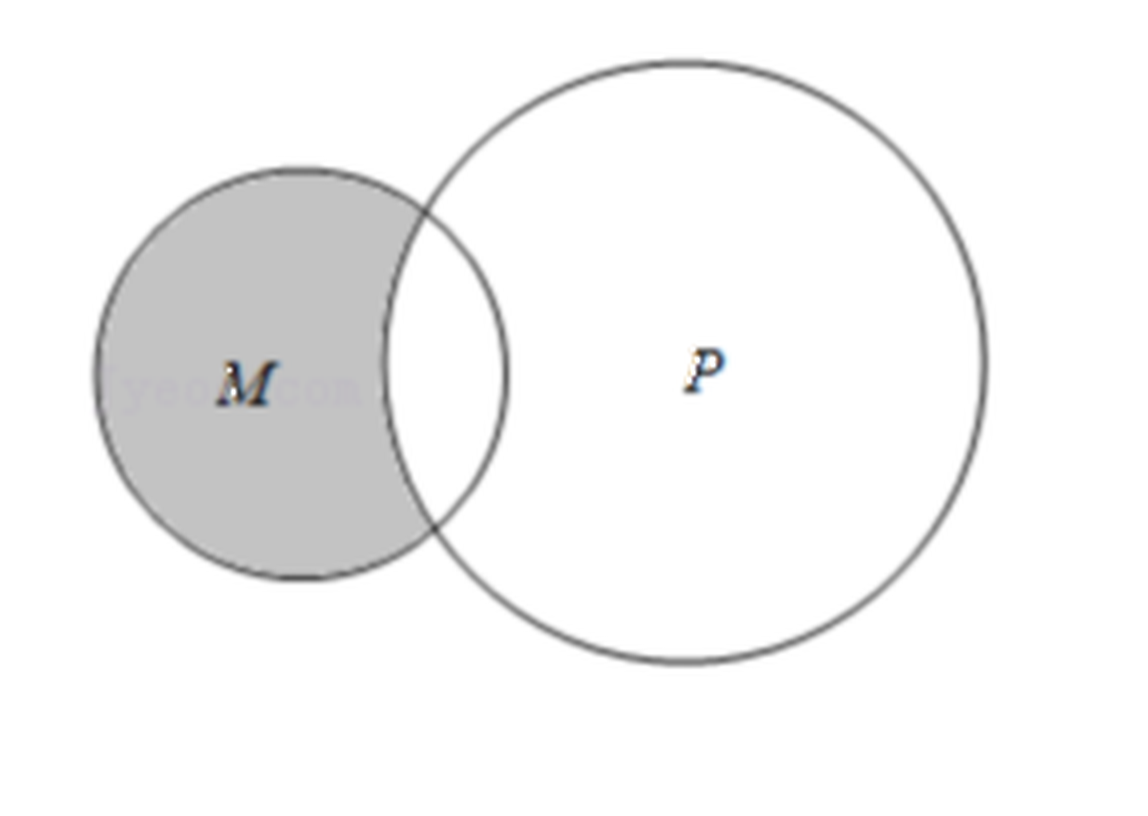
\includegraphics[width=0.36\textwidth]{figures/venn_M_shaded_P.png}
\end{center}

\step{阴影部分表示 $M-P$，所以 $M-(M-P)=M\cap P$. 故选 $B$.}
\solend

\fi

\item 设 $A_1$、$A_2$、$\cdots$、$A_7$ 均是含有 2 个元素的集合，且满足：

$A_i\cap A_{i+1}=\varnothing(i=1,2,3,4,5,6)$，$A_1\cap A_7=\varnothing$. 记 $B=A_1\cup A_2\cup\cdots\cup A_7$，则 $B$ 中元素个数的最小值是\mbox{（\quad）}

\keepwithprev
A. $4$\qquad B. $5$\qquad C. $6$\qquad D. $7$

\ans{$B$}

\ifanswer
\solbegin
\step{$A_1\cap A_7=\varnothing$，$A_i\cap A_{i+1}=\varnothing(i=1,2,3,4,5,6)$，}
\step{所以 $A_1$ 与 $A_2$ 的元素不同，则 $A_1\cup A_2$ 元素个数为 $4$，}
\step{若 $B$ 中元素个数的最小值是 $4$，则只能是 $A_3=A_1=A_5=A_7$，$A_4=A_2=A_6$，}
\step{与 $A_1\cap A_7=\varnothing$ 矛盾，}
\step{若 $A_3$ 从 $A_1$ 中选择 1 个元素，再加入一个新元素，}
\step{这样 $A_1\cup A_2\cup A_3$ 元素个数为 5 个，}
\step{这 5 个元素适当排列，得到 $A_4$、$A_5$、$A_6$、$A_7$，}
\step{例如 $A_1=\{1,2\},A_2=\{3,4\},A_3=\{1,5\}$，}
\step{取 $A_4=\{2,4\},A_5=\{3,5\},A_6=\{1,2\},A_7=\{3,5\}$，符合题意，}
\step{则 $B$ 中元素个数的最小值是 $2+2+1=5$，故选 $B$.}
\solend

\fi

\end{enumerate}

\bigsec{三、解答题}

\begin{enumerate}
\setcounter{enumi}{13}

\item 设 $A=\{x\mid x^2-ax+a^2-19=0\}$，$B=\{x\mid x^2-5x+6=0\}$，$C=\{x\mid x^2+2x-8=0\}$.

\begin{enumerate}[label=(\arabic*)]
\item 若 $A\cap B$ 非空，且 $A\cap C=\varnothing$，求 $a$ 的值；
\item $A\cap B=A\cap C\neq\varnothing$，求 $a$ 的值.
\end{enumerate}

\ifanswer
\solbegin
\stepm{(1)}{由题意，$C=\{-4,2\}$，}
\step{因为 $A\cap B$ 非空且 $A\cap C=\varnothing$，所以 $3\in A$，}
\step{即 $9-3a+a^2-19=0$，解得 $a=-2$ 或 $a=5$，}
\step{当 $a=-2$ 时，$A=\{3,-5\}$，满足题意；}
\step{当 $a=5$ 时，$A=\{2,3\}$，此时 $A\cap C=\{2\}$，不满足题意；}
\step{综上，$a=-2$；}
\stepm{(2)}{因为 $A\cap B=A\cap C\neq\varnothing$，所以 $2\in A$，}
\step{即 $4-2a+a^2-19=0$，解得 $a=-3$ 或 $a=5$，}
\step{当 $a=-3$ 时，$A=\{2,-5\}$，满足题意；}
\step{当 $a=5$ 时，$A=\{2,3\}$，不满足题意，}
\step{故 $a=-3$.}
\solend

\fi

\ansspace[6]

\item 已知 $A=\{x\mid x<-3\text{ 或 }x>1\}$.

\begin{enumerate}[label=(\arabic*)]
\item 若 $B=\{x\mid x<3m+1\text{ 或 }x>m+2\}$，$A\sub B$，求 $m$ 的取值范围.
\item 若 $B=\{x\mid m+2<x<3m+1\}$，$B\sub A$，求 $m$ 的取值范围.
\end{enumerate}

\ifanswer
\solbegin
\stepm{(1)}{当 $3m+1>m+2$，即 $m>\dfrac{1}{2}$ 时，$B=\R$，满足 $A\sub B$；}
\step{当 $3m+1\leqslant m+2$，即 $m\leqslant\dfrac{1}{2}$ 时，要使 $A\sub B$，}
\step{得 $\begin{cases}3m+1\geqslant-3\text{ ①}\\ m+2\leqslant 1\text{ ②}\end{cases}$，解得 $-\dfrac{4}{3}\leqslant m\leqslant-1$.}
\step{综上所述，$m$ 的取值范围为 $\left\{m\mid -\dfrac{4}{3}\leqslant m\leqslant-1\text{ 或 }m>\dfrac{1}{2}\right\}$；}
\stepm{(2)}{当 $B=\varnothing$ 时，则 $3m+1\leqslant m+2$，即 $m\leqslant\dfrac{1}{2}$ 时，满足 $B\sub A$；}
\step{当 $B\neq\varnothing$ 时，且 $B\sub A$，则 $\begin{cases}3m+1>m+2\\ 3m+1\leqslant-3\text{ 或 }m+2\geqslant 1\end{cases}$，所以 $m>\dfrac{1}{2}$.}
\step{综上所述，$m$ 的取值范围为 $\R$.}
\solend

\fi

\ansspace[6]

% 压轴题：其后已无内容，故作答区全用可丢弃胶水（\ansspace*），并在题目前先量一下版面。
\ansneed{7cm}

\item 已知集合 $A$ 为非空集合，定义

$S=\{x\mid x=a+b,a,b\in A\},T=\{x\mid x=|a-b|,a,b\in A\}$.

\begin{enumerate}[label=(\arabic*)]
\item 若集合 $A=\{1,3\}$，直接写出集合 $S$、$T$（无需写计算过程）；
\item 若集合 $A=\{x_1,x_2,x_3,x_4\}$，$x_1<x_2<x_3<x_4$，且 $T=A$，求证：$x_1+x_4=x_2+x_3$；
\item 若集合 $A=\{x\mid 0\leqslant x\leqslant 2021,x\in\N\}$，$S\cap T=\varnothing$. 记 $|A|$ 为集合 $A$ 中元素的个数，求 $|A|$ 的最大值.
\end{enumerate}

\ifanswer
\solbegin
\stepm{(1)}{$S=\{2,4,6\},T=\{0,2\}$；}
\stepm{(2)}{集合 $T$ 中最小的元素为 0，因为 $T=A$，且 $x_1<x_2<x_3<x_4$，所以 $x_1=0$，}
\step{所以集合 $T$ 中元素为 $x_2-x_1=x_2,x_3-x_1=x_3,x_4-x_1=x_4$，}
\step{以及 $x_3-x_2,x_4-x_2,x_4-x_3$ 均属于 $A$，}
% 注：本行原卷印「所以 $x_3$ 即 $x_4-x_2=x_3-x_1$」，「所以 $x_3$ 即 …」语义不完整，
%     疑有漏排（按本段结论应得 $x_4-x_2=x_3$），无法确证原意，本稿照抄原卷、未改。
\step{因为 $x_1=0<x_3-x_2<x_4-x_2<x_4$，所以 $x_3$ 即 $x_4-x_2=x_3-x_1$，}
\step{即 $x_1+x_4=x_2+x_3$；}
\stepm{(3)}{设 $A=\{a_1,a_2,a_3,\cdots,a_k\}$ 满足题意，其中 $a_1<a_2<\cdots<a_k$，}
\step{则 $2a_1<a_1+a_2<\cdots<a_1+a_k<a_2+a_k<a_3+a_k<\cdots<a_{k-1}+a_k<2a_k$，}
\step{所以 $|S\cup T|\leqslant 2k+1$，所以 $3k-1\leqslant 2a_k+1\leqslant 4043(k\in\N^*)$，}
\step{所以 $k\leqslant 1348$，}
\step{实际上当 $A=\{674,675,676,\cdots,2021\}$ 时满足题意，}
\step{证明如下：设 $A=\{m,m+1,m+2,\cdots,2021\},m\in\N$，}
\step{设 $S=\{2m,2m+1,2m+2,\cdots,4042\}$，$T=\{0,1,2,\cdots,2021-m\}$，}
\step{由题意得 $2021-m<2m$，即 $m>673\dfrac{2}{3}$，}
\step{故 $m$ 的最小值是 674，于是当 $m=674$，$A$ 中的元素最多，}
\step{即 $A=\{674,675,676,\cdots,2021\}$ 时满足题意，}
\step{综上所述，集合 $A$ 中元素的个数的最大值是 $1348$.}
\solend

\fi

\ansspace*[9]

\end{enumerate}

\bigsec{附加题}

\begin{enumerate}
\setcounter{enumi}{16}

\item 设 $A$ 是整数集的一个非空子集，对于 $k\in A$，如果 $k-1\notin A$ 且 $k+1\notin A$，那么 $k$ 是 $A$ 的一个“孤立元”。给定 $S=\{1,2,3,4,5,6,7,8\}$，由 $S$ 的 3 个元素构成的所有集合中，不含“孤立元”的集合共有 \blankline[2.4em] 个.

\ifanswer
\solbegin
\step{由题意得，“孤立元”即为在集合中无与之相邻的元素，}
\step{满足条件的集合有 $\{1,2,3\},\{2,3,4\},\{3,4,5\},\{4,5,6\},\{5,6,7\},\{6,7,8\}$，}
\step{共 6 个集合.}
\solend

\fi

\item 已知 $A\cap B=\varnothing$，$M=\{T\mid T\sub A\}$，$P=\{S\mid S\sub B\}$，则 $M\cap P=$ \blankline[4.4em].

\ans{$\{\varnothing\}$}

\item 已知集合 $A=\{x\mid x=m^2-n^2,m,n\in\Z\}$，写出所有满足集合 $A$ 的偶数 \blankline[4.4em].

\ans{$4n,n\in\Z$}

\item 对于给定的正整数 $n(n\geqslant 2)$ 若有限集合 $A=\{a_1,a_2,\cdots,a_n\}\sub M$，且满足

$a_1+a_2+\cdots+a_n=a_1\cdot a_2\cdots a_n$，则称 $A$ 为集合 $M$ 的 $n$ 元“调和子集”，则自然数集 $\N$ 的所有 3 元“调和子集”为 \blankline[3.6em].

\ans{$\{1,2,3\}$}

\end{enumerate}

\end{document}
"
% 紧凑版：xelatex "\def\iscompact{1}% 高一15_七宝中学_抱孩子练习.tex
%   —— 高一上数学「2026-2027 年七宝中学高一上抱孩子练习 9.8」（试卷版/答案版）
% 试卷版：xelatex 高一15_七宝中学_抱孩子练习.tex
% 答案版：xelatex "\def\isanswer{1}\input{高一15_七宝中学_抱孩子练习.tex}"
% 紧凑版：xelatex "\def\iscompact{1}\input{高一15_七宝中学_抱孩子练习.tex}"
%
% 原始材料是微信公众号图文（公众号「魔都数学加油站」），正文为 7 张 PNG 页（1080×1527）。
% 原文本身就是一份**讲评版**——题目下方直接印出【答案】或【解析】。试题文字、答案与解析
% 均照原卷录入，未改内容。卷面上的粉色斜水印「魔都数学加油站」属水印，未录入。
%
% 卷首标题：原卷印作「2026-2027 年七宝中学高一上抱孩子练习 9.8」——「抱孩子练习」四字
% 确系原卷所印（已放大 imgs_B/00.png 卷首核对），句末的「9.8」亦印在同一标题行内，
% 本稿一并照录，未改作「周末作业」；年份区间按全稿惯例排 en dash。
%
% 与原卷的排版差异（均已在 README「说明」中交代）：
%   ① 原文自**第 3 题**起（第 1、2 题未在该文中发布），故本稿题号亦自 3 起；
%   ② 原卷本就印有「一、填空题」「二、选择题」「三、解答题」三节标题，末节另印「附加题」，
%      本稿照原卷分节，只把标题改排成全稿统一的「大节标题」样式；
%   ③ 原卷填空、选择的答案直接印在题目下方，本稿统一改为试卷版隐去、答案版以【答案】或
%      【解析】给出（第 11 题原卷的答案是写在解析末句「故选 B」里的），使两版彻底分离；
%   ④ 原卷的集合符号 $R$、$Z$、$N$ 有正体与粗体两种写法（第 4 题的 $\mathbf{R}$、
%      第 16(3)、17、19、20 题的 $\mathbf{N}$、$\mathbf{Z}$ 为粗体，第 15 题解析的 $B=R$
%      为正体），本稿按全稿惯例统一写作 $\R$、$\Z$、$\N$；
%   ⑤ 原卷用**半角**括号（第 13 题「$\varnothing(i=1,2,3,4,5,6)$」、第 16(1)「(无需写计算过程)」、
%      第 16(2)「$A=\{x_1,x_2,x_3,x_4\}$」、第 20 题「$n(n\geqslant 2)$」），本稿按全稿惯例排全角；
%   ⑥ 原卷未印副标题，本稿按全稿惯例补出副标题「集合与常用逻辑用语」；
%   ⑦ 第 18、20 题的 $\subseteq$（带下划线，真包含写作 $\subset$ 与之形近）已逐处放大比对确认，
%      第 18 题的答案 $\{\varnothing\}$ 亦与 $\subseteq$ 口径相符（若为真包含则答案应为 $\varnothing$）。
%
% 原卷存疑两处（均已放大到能看清字形后核对，无法确证原意，本稿照抄原卷、未改）：
%   ① 第 10 题【解析】末句原卷印「所以 $1-k^2\neq 0$，即 $k\neq\pm 1$」——按此式，当 $k=1$
%      时两方程为同一直线、有无穷多解，$A\cap B\neq\varnothing$ 仍成立，故 $A\cap B\neq\varnothing$
%      当且仅当 $k\neq -1$；原卷结论与题设不合，疑为原卷笔误，但无法确证原意，本稿照抄原卷；
%   ② 第 16(2)【解析】原卷印「因为 $x_1=0<x_3-x_2<x_4-x_2<x_4$，所以 $x_3$ 即 $x_4-x_2=x_3-x_1$，」
%      ——「所以 $x_3$ 即 …」一句语义不完整，疑有漏排（按本段结论应得 $x_4-x_2=x_3$），
%      无法确证原意，本稿照抄原卷。

\documentclass[a4paper,11pt]{article}
\usepackage{common}

\begin{document}

\examtitlest[3]{2026--2027 年七宝中学高一上抱孩子练习 9.8}{集合与常用逻辑用语}

\bigsec{一、填空题}

\begin{enumerate}
\setcounter{enumi}{2}

\item 方程 $\sqrt{x+2}=-x$ 的解的集合为 \blankline[4.4em].

\ifanswer
\solbegin
\step{因为 $\sqrt{x+2}=-x$，所以 $\begin{cases}x\leqslant 0\\ x+2=x^2\end{cases}$，解得 $x=-1$，}
\step{所以方程 $\sqrt{x+2}=-x$ 的解的集合为 $\{-1\}$.}
\solend

\fi

\item 若 $A=\{x\mid a-4<x\leqslant a+4\}$，$B=\{x\mid x>5\text{ 或 }x<-1\}$，且 $A\cup B=\R$，则实数 $a$ 的取值范围是 \blankline[3.6em].

\ans{$[1,3)$}

\item 设集合 $A=\{x\mid x=2n+1,n\in\N\}$，$B=\{x\mid x=3n,n\in\N\}$，则 $A\cap B=$ \blankline[4.4em].

\ans{$\{x\mid x=6n+3,n\in\N\}$}

\item 已知集合 $A=\{1,2\}$，集合 $B=\{x\mid ax=6\}$，若 $A\cup B=A$，则 $a$ 的所有取值构成的集合为 \blankline[4.4em].

\ifanswer
\solbegin
\step{因为 $A\cup B=A$，所以 $B\sub A$，}
\step{当 $a=0$ 时，$B=\varnothing$，满足 $B\sub A$；}
\step{当 $a\neq 0$ 时，$B=\left\{\dfrac{6}{a}\right\}$，则 $\dfrac{6}{a}=1$ 或 $\dfrac{6}{a}=2$，解得 $a=6$ 或 $a=3$，}
\step{综上所述，$a$ 的所有取值构成的集合为 $\{0,3,6\}$.}
\solend

\fi

\item 设 $U=\{2,4,a^2-a+1\}$，$A=\{2,|a+1|\}$，$\overline{A}=\{7\}$，则 $a=$ \blankline[2.4em].

\ans{$3$}

\item 已知集合 $A=\{x\mid x^2-px-q=0\}$，$B=\{x\mid x^2+qx-p=0\}$，且 $A\cap B=\{1\}$，则 $A\cup B=$ \blankline[4.4em].

\ans{$\{0,-1,1\}$}

\item 定义集合运算：$A\odot B=\{z\mid z=xy(x+y),x\in A,y\in B\}$，若 $A=\{1,2\},B=\{3,4\}$，则 $A\odot B$ 的所有元素之和是 \blankline[3.6em].

\ans{$110$}

\item 已知集合 $A=\{(x,y)\mid kx+y=k+1\}$，$B=\{(x,y)\mid x+ky=2k\}$，其中 $k$ 为实数，$A\cap B\neq\varnothing$，则 $k$ 的取值范围是 \blankline[4.4em].

\ifanswer
\solbegin
\step{因为 $A\cap B\neq\varnothing$，所以方程组 $\begin{cases}kx+y=k+1\\ x+ky=2k\end{cases}$ 有解，消 $y$ 得 $(1-k^2)x=k-k^2$，}
% 注：末句原卷印「所以 $1-k^2\neq 0$，即 $k\neq\pm 1$」。按此式，$k=1$ 时两方程为同一直线、
%     有无穷多解，$A\cap B\neq\varnothing$ 仍成立，故结论应为 $k\neq -1$。疑为原卷笔误，
%     但无法确证原意，本稿照抄原卷、未改（详见文件头「原卷存疑」①）。
\step{所以 $1-k^2\neq 0$，即 $k\neq\pm 1$.}
\solend

\fi

\end{enumerate}

\bigsec{二、选择题}

\begin{enumerate}
\setcounter{enumi}{10}

\item 给出关系式：①$0\in\varnothing$；②$\varnothing=\{0\}$；③$\{a,b\}=\{b,a\}$；④$\{y\mid y=x^2-2\}=\{(x,y)\mid y=x^2-2\}$，其中正确的关系式的个数是\mbox{（\quad）}

\keepwithprev
A. $0$\qquad B. $1$\qquad C. $2$\qquad D. $3$

\ans{$B$}

\ifanswer
\solbegin
\step{在①中，$\varnothing$ 表示空集，$0\notin\varnothing$，故①错误；在②中，$\varnothing\sub\{0\}$，故②错误；}
\step{在③中，$\{a,b\}=\{b,a\}$，故③正确；}
\step{在④中，因为，$\{y\mid y=x^2-2\}$ 和 $\{(x,y)\mid y=x^2-2\}$ 的代表元素不同，}
\step{所以 $\{y\mid y=x^2-2\}\neq\{(x,y)\mid y=x^2-2\}$，故④错误.}
\step{故正确的是③，故选 $B$.}
\solend

\fi

\item 设集合 $M$、$P\neq\varnothing$，定义集合 $M-P=\{x\mid x\in M,x\notin P\}$，则集合 $M-(M-P)$ 是\mbox{（\quad）}

\keepwithprev
A. $P$\qquad B. $M$\qquad C. $M\cup P$\qquad D. $M\cap P$

\ans{$B$}

\ifanswer
\solbegin
\step{$M-(M-P)=\{x\mid x\in M,\text{ 且 }x\notin(M-P)\}$，}
\step{用 venn 图表示集合 $M$、$P$ 的关系如图：}

\begin{center}
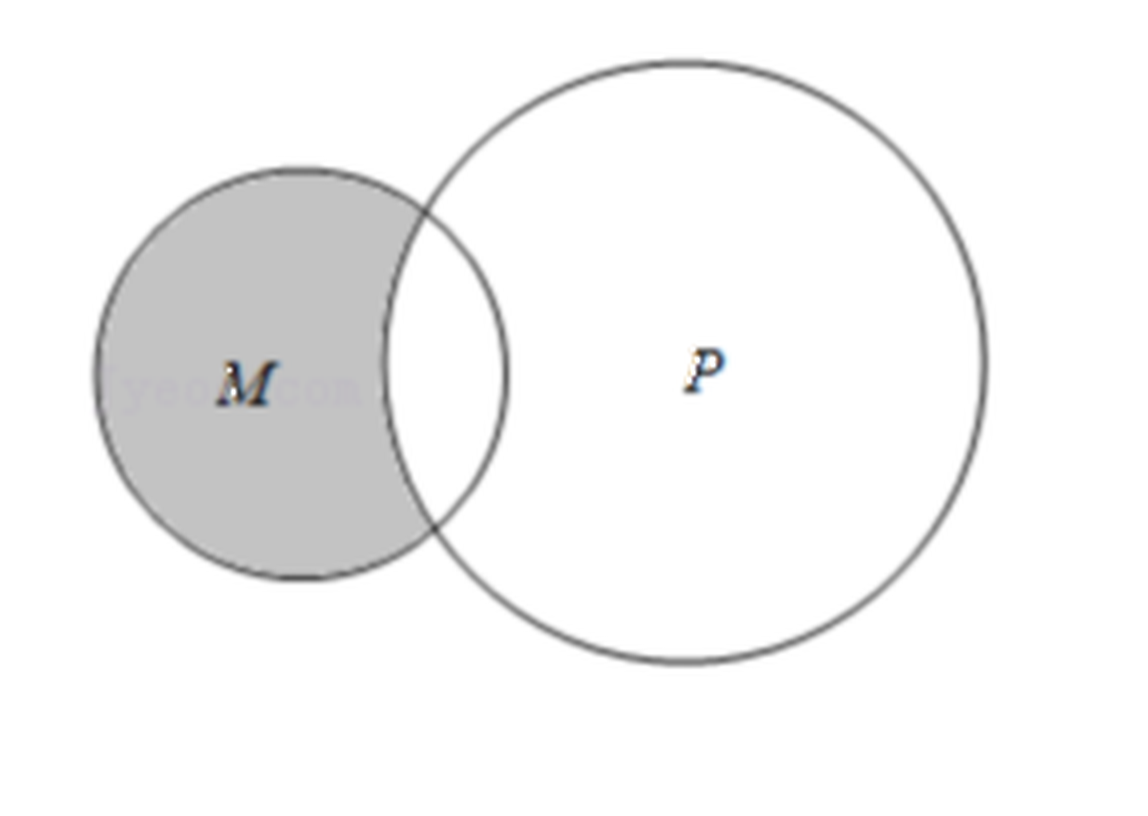
\includegraphics[width=0.36\textwidth]{figures/venn_M_shaded_P.png}
\end{center}

\step{阴影部分表示 $M-P$，所以 $M-(M-P)=M\cap P$. 故选 $B$.}
\solend

\fi

\item 设 $A_1$、$A_2$、$\cdots$、$A_7$ 均是含有 2 个元素的集合，且满足：

$A_i\cap A_{i+1}=\varnothing(i=1,2,3,4,5,6)$，$A_1\cap A_7=\varnothing$. 记 $B=A_1\cup A_2\cup\cdots\cup A_7$，则 $B$ 中元素个数的最小值是\mbox{（\quad）}

\keepwithprev
A. $4$\qquad B. $5$\qquad C. $6$\qquad D. $7$

\ans{$B$}

\ifanswer
\solbegin
\step{$A_1\cap A_7=\varnothing$，$A_i\cap A_{i+1}=\varnothing(i=1,2,3,4,5,6)$，}
\step{所以 $A_1$ 与 $A_2$ 的元素不同，则 $A_1\cup A_2$ 元素个数为 $4$，}
\step{若 $B$ 中元素个数的最小值是 $4$，则只能是 $A_3=A_1=A_5=A_7$，$A_4=A_2=A_6$，}
\step{与 $A_1\cap A_7=\varnothing$ 矛盾，}
\step{若 $A_3$ 从 $A_1$ 中选择 1 个元素，再加入一个新元素，}
\step{这样 $A_1\cup A_2\cup A_3$ 元素个数为 5 个，}
\step{这 5 个元素适当排列，得到 $A_4$、$A_5$、$A_6$、$A_7$，}
\step{例如 $A_1=\{1,2\},A_2=\{3,4\},A_3=\{1,5\}$，}
\step{取 $A_4=\{2,4\},A_5=\{3,5\},A_6=\{1,2\},A_7=\{3,5\}$，符合题意，}
\step{则 $B$ 中元素个数的最小值是 $2+2+1=5$，故选 $B$.}
\solend

\fi

\end{enumerate}

\bigsec{三、解答题}

\begin{enumerate}
\setcounter{enumi}{13}

\item 设 $A=\{x\mid x^2-ax+a^2-19=0\}$，$B=\{x\mid x^2-5x+6=0\}$，$C=\{x\mid x^2+2x-8=0\}$.

\begin{enumerate}[label=(\arabic*)]
\item 若 $A\cap B$ 非空，且 $A\cap C=\varnothing$，求 $a$ 的值；
\item $A\cap B=A\cap C\neq\varnothing$，求 $a$ 的值.
\end{enumerate}

\ifanswer
\solbegin
\stepm{(1)}{由题意，$C=\{-4,2\}$，}
\step{因为 $A\cap B$ 非空且 $A\cap C=\varnothing$，所以 $3\in A$，}
\step{即 $9-3a+a^2-19=0$，解得 $a=-2$ 或 $a=5$，}
\step{当 $a=-2$ 时，$A=\{3,-5\}$，满足题意；}
\step{当 $a=5$ 时，$A=\{2,3\}$，此时 $A\cap C=\{2\}$，不满足题意；}
\step{综上，$a=-2$；}
\stepm{(2)}{因为 $A\cap B=A\cap C\neq\varnothing$，所以 $2\in A$，}
\step{即 $4-2a+a^2-19=0$，解得 $a=-3$ 或 $a=5$，}
\step{当 $a=-3$ 时，$A=\{2,-5\}$，满足题意；}
\step{当 $a=5$ 时，$A=\{2,3\}$，不满足题意，}
\step{故 $a=-3$.}
\solend

\fi

\ansspace[6]

\item 已知 $A=\{x\mid x<-3\text{ 或 }x>1\}$.

\begin{enumerate}[label=(\arabic*)]
\item 若 $B=\{x\mid x<3m+1\text{ 或 }x>m+2\}$，$A\sub B$，求 $m$ 的取值范围.
\item 若 $B=\{x\mid m+2<x<3m+1\}$，$B\sub A$，求 $m$ 的取值范围.
\end{enumerate}

\ifanswer
\solbegin
\stepm{(1)}{当 $3m+1>m+2$，即 $m>\dfrac{1}{2}$ 时，$B=\R$，满足 $A\sub B$；}
\step{当 $3m+1\leqslant m+2$，即 $m\leqslant\dfrac{1}{2}$ 时，要使 $A\sub B$，}
\step{得 $\begin{cases}3m+1\geqslant-3\text{ ①}\\ m+2\leqslant 1\text{ ②}\end{cases}$，解得 $-\dfrac{4}{3}\leqslant m\leqslant-1$.}
\step{综上所述，$m$ 的取值范围为 $\left\{m\mid -\dfrac{4}{3}\leqslant m\leqslant-1\text{ 或 }m>\dfrac{1}{2}\right\}$；}
\stepm{(2)}{当 $B=\varnothing$ 时，则 $3m+1\leqslant m+2$，即 $m\leqslant\dfrac{1}{2}$ 时，满足 $B\sub A$；}
\step{当 $B\neq\varnothing$ 时，且 $B\sub A$，则 $\begin{cases}3m+1>m+2\\ 3m+1\leqslant-3\text{ 或 }m+2\geqslant 1\end{cases}$，所以 $m>\dfrac{1}{2}$.}
\step{综上所述，$m$ 的取值范围为 $\R$.}
\solend

\fi

\ansspace[6]

% 压轴题：其后已无内容，故作答区全用可丢弃胶水（\ansspace*），并在题目前先量一下版面。
\ansneed{7cm}

\item 已知集合 $A$ 为非空集合，定义

$S=\{x\mid x=a+b,a,b\in A\},T=\{x\mid x=|a-b|,a,b\in A\}$.

\begin{enumerate}[label=(\arabic*)]
\item 若集合 $A=\{1,3\}$，直接写出集合 $S$、$T$（无需写计算过程）；
\item 若集合 $A=\{x_1,x_2,x_3,x_4\}$，$x_1<x_2<x_3<x_4$，且 $T=A$，求证：$x_1+x_4=x_2+x_3$；
\item 若集合 $A=\{x\mid 0\leqslant x\leqslant 2021,x\in\N\}$，$S\cap T=\varnothing$. 记 $|A|$ 为集合 $A$ 中元素的个数，求 $|A|$ 的最大值.
\end{enumerate}

\ifanswer
\solbegin
\stepm{(1)}{$S=\{2,4,6\},T=\{0,2\}$；}
\stepm{(2)}{集合 $T$ 中最小的元素为 0，因为 $T=A$，且 $x_1<x_2<x_3<x_4$，所以 $x_1=0$，}
\step{所以集合 $T$ 中元素为 $x_2-x_1=x_2,x_3-x_1=x_3,x_4-x_1=x_4$，}
\step{以及 $x_3-x_2,x_4-x_2,x_4-x_3$ 均属于 $A$，}
% 注：本行原卷印「所以 $x_3$ 即 $x_4-x_2=x_3-x_1$」，「所以 $x_3$ 即 …」语义不完整，
%     疑有漏排（按本段结论应得 $x_4-x_2=x_3$），无法确证原意，本稿照抄原卷、未改。
\step{因为 $x_1=0<x_3-x_2<x_4-x_2<x_4$，所以 $x_3$ 即 $x_4-x_2=x_3-x_1$，}
\step{即 $x_1+x_4=x_2+x_3$；}
\stepm{(3)}{设 $A=\{a_1,a_2,a_3,\cdots,a_k\}$ 满足题意，其中 $a_1<a_2<\cdots<a_k$，}
\step{则 $2a_1<a_1+a_2<\cdots<a_1+a_k<a_2+a_k<a_3+a_k<\cdots<a_{k-1}+a_k<2a_k$，}
\step{所以 $|S\cup T|\leqslant 2k+1$，所以 $3k-1\leqslant 2a_k+1\leqslant 4043(k\in\N^*)$，}
\step{所以 $k\leqslant 1348$，}
\step{实际上当 $A=\{674,675,676,\cdots,2021\}$ 时满足题意，}
\step{证明如下：设 $A=\{m,m+1,m+2,\cdots,2021\},m\in\N$，}
\step{设 $S=\{2m,2m+1,2m+2,\cdots,4042\}$，$T=\{0,1,2,\cdots,2021-m\}$，}
\step{由题意得 $2021-m<2m$，即 $m>673\dfrac{2}{3}$，}
\step{故 $m$ 的最小值是 674，于是当 $m=674$，$A$ 中的元素最多，}
\step{即 $A=\{674,675,676,\cdots,2021\}$ 时满足题意，}
\step{综上所述，集合 $A$ 中元素的个数的最大值是 $1348$.}
\solend

\fi

\ansspace*[9]

\end{enumerate}

\bigsec{附加题}

\begin{enumerate}
\setcounter{enumi}{16}

\item 设 $A$ 是整数集的一个非空子集，对于 $k\in A$，如果 $k-1\notin A$ 且 $k+1\notin A$，那么 $k$ 是 $A$ 的一个“孤立元”。给定 $S=\{1,2,3,4,5,6,7,8\}$，由 $S$ 的 3 个元素构成的所有集合中，不含“孤立元”的集合共有 \blankline[2.4em] 个.

\ifanswer
\solbegin
\step{由题意得，“孤立元”即为在集合中无与之相邻的元素，}
\step{满足条件的集合有 $\{1,2,3\},\{2,3,4\},\{3,4,5\},\{4,5,6\},\{5,6,7\},\{6,7,8\}$，}
\step{共 6 个集合.}
\solend

\fi

\item 已知 $A\cap B=\varnothing$，$M=\{T\mid T\sub A\}$，$P=\{S\mid S\sub B\}$，则 $M\cap P=$ \blankline[4.4em].

\ans{$\{\varnothing\}$}

\item 已知集合 $A=\{x\mid x=m^2-n^2,m,n\in\Z\}$，写出所有满足集合 $A$ 的偶数 \blankline[4.4em].

\ans{$4n,n\in\Z$}

\item 对于给定的正整数 $n(n\geqslant 2)$ 若有限集合 $A=\{a_1,a_2,\cdots,a_n\}\sub M$，且满足

$a_1+a_2+\cdots+a_n=a_1\cdot a_2\cdots a_n$，则称 $A$ 为集合 $M$ 的 $n$ 元“调和子集”，则自然数集 $\N$ 的所有 3 元“调和子集”为 \blankline[3.6em].

\ans{$\{1,2,3\}$}

\end{enumerate}

\end{document}
"
%
% 原始材料是微信公众号图文（公众号「魔都数学加油站」），正文为 7 张 PNG 页（1080×1527）。
% 原文本身就是一份**讲评版**——题目下方直接印出【答案】或【解析】。试题文字、答案与解析
% 均照原卷录入，未改内容。卷面上的粉色斜水印「魔都数学加油站」属水印，未录入。
%
% 卷首标题：原卷印作「2026-2027 年七宝中学高一上抱孩子练习 9.8」——「抱孩子练习」四字
% 确系原卷所印（已放大 imgs_B/00.png 卷首核对），句末的「9.8」亦印在同一标题行内，
% 本稿一并照录，未改作「周末作业」；年份区间按全稿惯例排 en dash。
%
% 与原卷的排版差异（均已在 README「说明」中交代）：
%   ① 原文自**第 3 题**起（第 1、2 题未在该文中发布），故本稿题号亦自 3 起；
%   ② 原卷本就印有「一、填空题」「二、选择题」「三、解答题」三节标题，末节另印「附加题」，
%      本稿照原卷分节，只把标题改排成全稿统一的「大节标题」样式；
%   ③ 原卷填空、选择的答案直接印在题目下方，本稿统一改为试卷版隐去、答案版以【答案】或
%      【解析】给出（第 11 题原卷的答案是写在解析末句「故选 B」里的），使两版彻底分离；
%   ④ 原卷的集合符号 $R$、$Z$、$N$ 有正体与粗体两种写法（第 4 题的 $\mathbf{R}$、
%      第 16(3)、17、19、20 题的 $\mathbf{N}$、$\mathbf{Z}$ 为粗体，第 15 题解析的 $B=R$
%      为正体），本稿按全稿惯例统一写作 $\R$、$\Z$、$\N$；
%   ⑤ 原卷用**半角**括号（第 13 题「$\varnothing(i=1,2,3,4,5,6)$」、第 16(1)「(无需写计算过程)」、
%      第 16(2)「$A=\{x_1,x_2,x_3,x_4\}$」、第 20 题「$n(n\geqslant 2)$」），本稿按全稿惯例排全角；
%   ⑥ 原卷未印副标题，本稿按全稿惯例补出副标题「集合与常用逻辑用语」；
%   ⑦ 第 18、20 题的 $\subseteq$（带下划线，真包含写作 $\subset$ 与之形近）已逐处放大比对确认，
%      第 18 题的答案 $\{\varnothing\}$ 亦与 $\subseteq$ 口径相符（若为真包含则答案应为 $\varnothing$）。
%
% 原卷存疑两处（均已放大到能看清字形后核对，无法确证原意，本稿照抄原卷、未改）：
%   ① 第 10 题【解析】末句原卷印「所以 $1-k^2\neq 0$，即 $k\neq\pm 1$」——按此式，当 $k=1$
%      时两方程为同一直线、有无穷多解，$A\cap B\neq\varnothing$ 仍成立，故 $A\cap B\neq\varnothing$
%      当且仅当 $k\neq -1$；原卷结论与题设不合，疑为原卷笔误，但无法确证原意，本稿照抄原卷；
%   ② 第 16(2)【解析】原卷印「因为 $x_1=0<x_3-x_2<x_4-x_2<x_4$，所以 $x_3$ 即 $x_4-x_2=x_3-x_1$，」
%      ——「所以 $x_3$ 即 …」一句语义不完整，疑有漏排（按本段结论应得 $x_4-x_2=x_3$），
%      无法确证原意，本稿照抄原卷。

\documentclass[a4paper,11pt]{article}
\usepackage{common}

\begin{document}

\examtitlest[3]{2026--2027 年七宝中学高一上抱孩子练习 9.8}{集合与常用逻辑用语}

\bigsec{一、填空题}

\begin{enumerate}
\setcounter{enumi}{2}

\item 方程 $\sqrt{x+2}=-x$ 的解的集合为 \blankline[4.4em].

\ifanswer
\solbegin
\step{因为 $\sqrt{x+2}=-x$，所以 $\begin{cases}x\leqslant 0\\ x+2=x^2\end{cases}$，解得 $x=-1$，}
\step{所以方程 $\sqrt{x+2}=-x$ 的解的集合为 $\{-1\}$.}
\solend

\fi

\item 若 $A=\{x\mid a-4<x\leqslant a+4\}$，$B=\{x\mid x>5\text{ 或 }x<-1\}$，且 $A\cup B=\R$，则实数 $a$ 的取值范围是 \blankline[3.6em].

\ans{$[1,3)$}

\item 设集合 $A=\{x\mid x=2n+1,n\in\N\}$，$B=\{x\mid x=3n,n\in\N\}$，则 $A\cap B=$ \blankline[4.4em].

\ans{$\{x\mid x=6n+3,n\in\N\}$}

\item 已知集合 $A=\{1,2\}$，集合 $B=\{x\mid ax=6\}$，若 $A\cup B=A$，则 $a$ 的所有取值构成的集合为 \blankline[4.4em].

\ifanswer
\solbegin
\step{因为 $A\cup B=A$，所以 $B\sub A$，}
\step{当 $a=0$ 时，$B=\varnothing$，满足 $B\sub A$；}
\step{当 $a\neq 0$ 时，$B=\left\{\dfrac{6}{a}\right\}$，则 $\dfrac{6}{a}=1$ 或 $\dfrac{6}{a}=2$，解得 $a=6$ 或 $a=3$，}
\step{综上所述，$a$ 的所有取值构成的集合为 $\{0,3,6\}$.}
\solend

\fi

\item 设 $U=\{2,4,a^2-a+1\}$，$A=\{2,|a+1|\}$，$\overline{A}=\{7\}$，则 $a=$ \blankline[2.4em].

\ans{$3$}

\item 已知集合 $A=\{x\mid x^2-px-q=0\}$，$B=\{x\mid x^2+qx-p=0\}$，且 $A\cap B=\{1\}$，则 $A\cup B=$ \blankline[4.4em].

\ans{$\{0,-1,1\}$}

\item 定义集合运算：$A\odot B=\{z\mid z=xy(x+y),x\in A,y\in B\}$，若 $A=\{1,2\},B=\{3,4\}$，则 $A\odot B$ 的所有元素之和是 \blankline[3.6em].

\ans{$110$}

\item 已知集合 $A=\{(x,y)\mid kx+y=k+1\}$，$B=\{(x,y)\mid x+ky=2k\}$，其中 $k$ 为实数，$A\cap B\neq\varnothing$，则 $k$ 的取值范围是 \blankline[4.4em].

\ifanswer
\solbegin
\step{因为 $A\cap B\neq\varnothing$，所以方程组 $\begin{cases}kx+y=k+1\\ x+ky=2k\end{cases}$ 有解，消 $y$ 得 $(1-k^2)x=k-k^2$，}
% 注：末句原卷印「所以 $1-k^2\neq 0$，即 $k\neq\pm 1$」。按此式，$k=1$ 时两方程为同一直线、
%     有无穷多解，$A\cap B\neq\varnothing$ 仍成立，故结论应为 $k\neq -1$。疑为原卷笔误，
%     但无法确证原意，本稿照抄原卷、未改（详见文件头「原卷存疑」①）。
\step{所以 $1-k^2\neq 0$，即 $k\neq\pm 1$.}
\solend

\fi

\end{enumerate}

\bigsec{二、选择题}

\begin{enumerate}
\setcounter{enumi}{10}

\item 给出关系式：①$0\in\varnothing$；②$\varnothing=\{0\}$；③$\{a,b\}=\{b,a\}$；④$\{y\mid y=x^2-2\}=\{(x,y)\mid y=x^2-2\}$，其中正确的关系式的个数是\mbox{（\quad）}

\keepwithprev
A. $0$\qquad B. $1$\qquad C. $2$\qquad D. $3$

\ans{$B$}

\ifanswer
\solbegin
\step{在①中，$\varnothing$ 表示空集，$0\notin\varnothing$，故①错误；在②中，$\varnothing\sub\{0\}$，故②错误；}
\step{在③中，$\{a,b\}=\{b,a\}$，故③正确；}
\step{在④中，因为，$\{y\mid y=x^2-2\}$ 和 $\{(x,y)\mid y=x^2-2\}$ 的代表元素不同，}
\step{所以 $\{y\mid y=x^2-2\}\neq\{(x,y)\mid y=x^2-2\}$，故④错误.}
\step{故正确的是③，故选 $B$.}
\solend

\fi

\item 设集合 $M$、$P\neq\varnothing$，定义集合 $M-P=\{x\mid x\in M,x\notin P\}$，则集合 $M-(M-P)$ 是\mbox{（\quad）}

\keepwithprev
A. $P$\qquad B. $M$\qquad C. $M\cup P$\qquad D. $M\cap P$

\ans{$B$}

\ifanswer
\solbegin
\step{$M-(M-P)=\{x\mid x\in M,\text{ 且 }x\notin(M-P)\}$，}
\step{用 venn 图表示集合 $M$、$P$ 的关系如图：}

\begin{center}
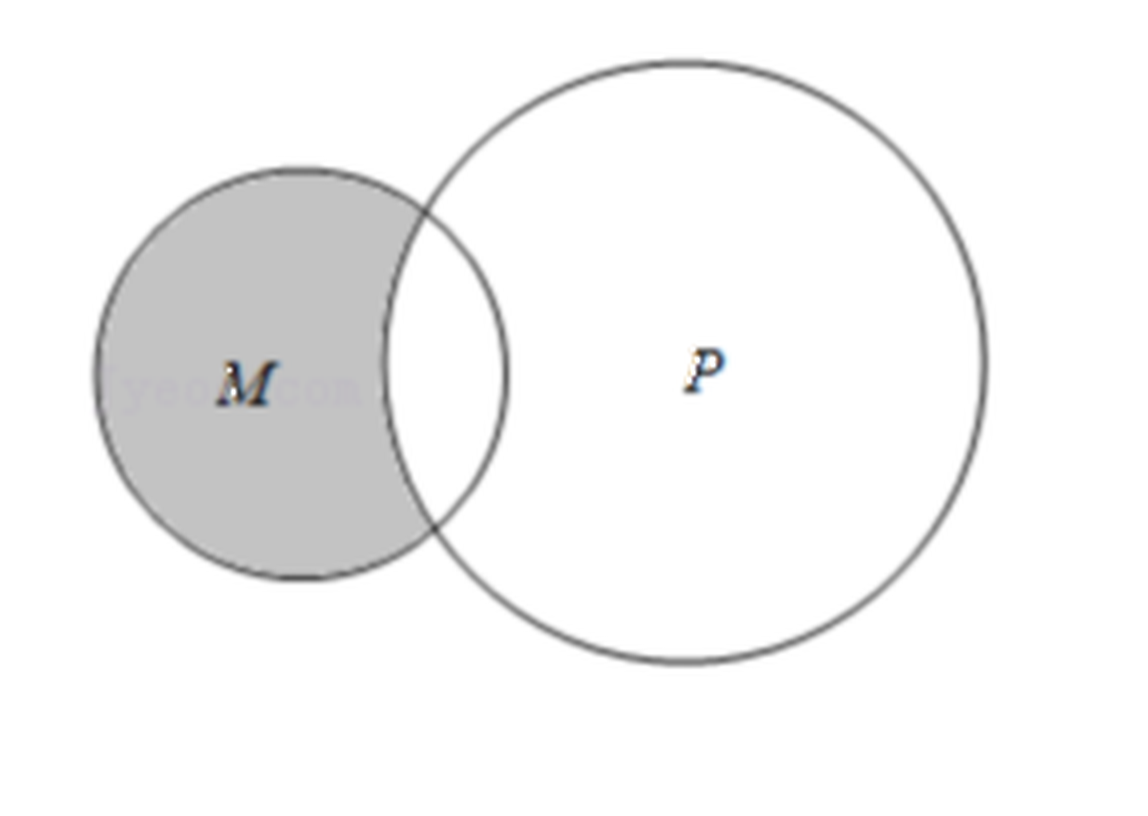
\includegraphics[width=0.36\textwidth]{figures/venn_M_shaded_P.png}
\end{center}

\step{阴影部分表示 $M-P$，所以 $M-(M-P)=M\cap P$. 故选 $B$.}
\solend

\fi

\item 设 $A_1$、$A_2$、$\cdots$、$A_7$ 均是含有 2 个元素的集合，且满足：

$A_i\cap A_{i+1}=\varnothing(i=1,2,3,4,5,6)$，$A_1\cap A_7=\varnothing$. 记 $B=A_1\cup A_2\cup\cdots\cup A_7$，则 $B$ 中元素个数的最小值是\mbox{（\quad）}

\keepwithprev
A. $4$\qquad B. $5$\qquad C. $6$\qquad D. $7$

\ans{$B$}

\ifanswer
\solbegin
\step{$A_1\cap A_7=\varnothing$，$A_i\cap A_{i+1}=\varnothing(i=1,2,3,4,5,6)$，}
\step{所以 $A_1$ 与 $A_2$ 的元素不同，则 $A_1\cup A_2$ 元素个数为 $4$，}
\step{若 $B$ 中元素个数的最小值是 $4$，则只能是 $A_3=A_1=A_5=A_7$，$A_4=A_2=A_6$，}
\step{与 $A_1\cap A_7=\varnothing$ 矛盾，}
\step{若 $A_3$ 从 $A_1$ 中选择 1 个元素，再加入一个新元素，}
\step{这样 $A_1\cup A_2\cup A_3$ 元素个数为 5 个，}
\step{这 5 个元素适当排列，得到 $A_4$、$A_5$、$A_6$、$A_7$，}
\step{例如 $A_1=\{1,2\},A_2=\{3,4\},A_3=\{1,5\}$，}
\step{取 $A_4=\{2,4\},A_5=\{3,5\},A_6=\{1,2\},A_7=\{3,5\}$，符合题意，}
\step{则 $B$ 中元素个数的最小值是 $2+2+1=5$，故选 $B$.}
\solend

\fi

\end{enumerate}

\bigsec{三、解答题}

\begin{enumerate}
\setcounter{enumi}{13}

\item 设 $A=\{x\mid x^2-ax+a^2-19=0\}$，$B=\{x\mid x^2-5x+6=0\}$，$C=\{x\mid x^2+2x-8=0\}$.

\begin{enumerate}[label=(\arabic*)]
\item 若 $A\cap B$ 非空，且 $A\cap C=\varnothing$，求 $a$ 的值；
\item $A\cap B=A\cap C\neq\varnothing$，求 $a$ 的值.
\end{enumerate}

\ifanswer
\solbegin
\stepm{(1)}{由题意，$C=\{-4,2\}$，}
\step{因为 $A\cap B$ 非空且 $A\cap C=\varnothing$，所以 $3\in A$，}
\step{即 $9-3a+a^2-19=0$，解得 $a=-2$ 或 $a=5$，}
\step{当 $a=-2$ 时，$A=\{3,-5\}$，满足题意；}
\step{当 $a=5$ 时，$A=\{2,3\}$，此时 $A\cap C=\{2\}$，不满足题意；}
\step{综上，$a=-2$；}
\stepm{(2)}{因为 $A\cap B=A\cap C\neq\varnothing$，所以 $2\in A$，}
\step{即 $4-2a+a^2-19=0$，解得 $a=-3$ 或 $a=5$，}
\step{当 $a=-3$ 时，$A=\{2,-5\}$，满足题意；}
\step{当 $a=5$ 时，$A=\{2,3\}$，不满足题意，}
\step{故 $a=-3$.}
\solend

\fi

\ansspace[6]

\item 已知 $A=\{x\mid x<-3\text{ 或 }x>1\}$.

\begin{enumerate}[label=(\arabic*)]
\item 若 $B=\{x\mid x<3m+1\text{ 或 }x>m+2\}$，$A\sub B$，求 $m$ 的取值范围.
\item 若 $B=\{x\mid m+2<x<3m+1\}$，$B\sub A$，求 $m$ 的取值范围.
\end{enumerate}

\ifanswer
\solbegin
\stepm{(1)}{当 $3m+1>m+2$，即 $m>\dfrac{1}{2}$ 时，$B=\R$，满足 $A\sub B$；}
\step{当 $3m+1\leqslant m+2$，即 $m\leqslant\dfrac{1}{2}$ 时，要使 $A\sub B$，}
\step{得 $\begin{cases}3m+1\geqslant-3\text{ ①}\\ m+2\leqslant 1\text{ ②}\end{cases}$，解得 $-\dfrac{4}{3}\leqslant m\leqslant-1$.}
\step{综上所述，$m$ 的取值范围为 $\left\{m\mid -\dfrac{4}{3}\leqslant m\leqslant-1\text{ 或 }m>\dfrac{1}{2}\right\}$；}
\stepm{(2)}{当 $B=\varnothing$ 时，则 $3m+1\leqslant m+2$，即 $m\leqslant\dfrac{1}{2}$ 时，满足 $B\sub A$；}
\step{当 $B\neq\varnothing$ 时，且 $B\sub A$，则 $\begin{cases}3m+1>m+2\\ 3m+1\leqslant-3\text{ 或 }m+2\geqslant 1\end{cases}$，所以 $m>\dfrac{1}{2}$.}
\step{综上所述，$m$ 的取值范围为 $\R$.}
\solend

\fi

\ansspace[6]

% 压轴题：其后已无内容，故作答区全用可丢弃胶水（\ansspace*），并在题目前先量一下版面。
\ansneed{7cm}

\item 已知集合 $A$ 为非空集合，定义

$S=\{x\mid x=a+b,a,b\in A\},T=\{x\mid x=|a-b|,a,b\in A\}$.

\begin{enumerate}[label=(\arabic*)]
\item 若集合 $A=\{1,3\}$，直接写出集合 $S$、$T$（无需写计算过程）；
\item 若集合 $A=\{x_1,x_2,x_3,x_4\}$，$x_1<x_2<x_3<x_4$，且 $T=A$，求证：$x_1+x_4=x_2+x_3$；
\item 若集合 $A=\{x\mid 0\leqslant x\leqslant 2021,x\in\N\}$，$S\cap T=\varnothing$. 记 $|A|$ 为集合 $A$ 中元素的个数，求 $|A|$ 的最大值.
\end{enumerate}

\ifanswer
\solbegin
\stepm{(1)}{$S=\{2,4,6\},T=\{0,2\}$；}
\stepm{(2)}{集合 $T$ 中最小的元素为 0，因为 $T=A$，且 $x_1<x_2<x_3<x_4$，所以 $x_1=0$，}
\step{所以集合 $T$ 中元素为 $x_2-x_1=x_2,x_3-x_1=x_3,x_4-x_1=x_4$，}
\step{以及 $x_3-x_2,x_4-x_2,x_4-x_3$ 均属于 $A$，}
% 注：本行原卷印「所以 $x_3$ 即 $x_4-x_2=x_3-x_1$」，「所以 $x_3$ 即 …」语义不完整，
%     疑有漏排（按本段结论应得 $x_4-x_2=x_3$），无法确证原意，本稿照抄原卷、未改。
\step{因为 $x_1=0<x_3-x_2<x_4-x_2<x_4$，所以 $x_3$ 即 $x_4-x_2=x_3-x_1$，}
\step{即 $x_1+x_4=x_2+x_3$；}
\stepm{(3)}{设 $A=\{a_1,a_2,a_3,\cdots,a_k\}$ 满足题意，其中 $a_1<a_2<\cdots<a_k$，}
\step{则 $2a_1<a_1+a_2<\cdots<a_1+a_k<a_2+a_k<a_3+a_k<\cdots<a_{k-1}+a_k<2a_k$，}
\step{所以 $|S\cup T|\leqslant 2k+1$，所以 $3k-1\leqslant 2a_k+1\leqslant 4043(k\in\N^*)$，}
\step{所以 $k\leqslant 1348$，}
\step{实际上当 $A=\{674,675,676,\cdots,2021\}$ 时满足题意，}
\step{证明如下：设 $A=\{m,m+1,m+2,\cdots,2021\},m\in\N$，}
\step{设 $S=\{2m,2m+1,2m+2,\cdots,4042\}$，$T=\{0,1,2,\cdots,2021-m\}$，}
\step{由题意得 $2021-m<2m$，即 $m>673\dfrac{2}{3}$，}
\step{故 $m$ 的最小值是 674，于是当 $m=674$，$A$ 中的元素最多，}
\step{即 $A=\{674,675,676,\cdots,2021\}$ 时满足题意，}
\step{综上所述，集合 $A$ 中元素的个数的最大值是 $1348$.}
\solend

\fi

\ansspace*[9]

\end{enumerate}

\bigsec{附加题}

\begin{enumerate}
\setcounter{enumi}{16}

\item 设 $A$ 是整数集的一个非空子集，对于 $k\in A$，如果 $k-1\notin A$ 且 $k+1\notin A$，那么 $k$ 是 $A$ 的一个“孤立元”。给定 $S=\{1,2,3,4,5,6,7,8\}$，由 $S$ 的 3 个元素构成的所有集合中，不含“孤立元”的集合共有 \blankline[2.4em] 个.

\ifanswer
\solbegin
\step{由题意得，“孤立元”即为在集合中无与之相邻的元素，}
\step{满足条件的集合有 $\{1,2,3\},\{2,3,4\},\{3,4,5\},\{4,5,6\},\{5,6,7\},\{6,7,8\}$，}
\step{共 6 个集合.}
\solend

\fi

\item 已知 $A\cap B=\varnothing$，$M=\{T\mid T\sub A\}$，$P=\{S\mid S\sub B\}$，则 $M\cap P=$ \blankline[4.4em].

\ans{$\{\varnothing\}$}

\item 已知集合 $A=\{x\mid x=m^2-n^2,m,n\in\Z\}$，写出所有满足集合 $A$ 的偶数 \blankline[4.4em].

\ans{$4n,n\in\Z$}

\item 对于给定的正整数 $n(n\geqslant 2)$ 若有限集合 $A=\{a_1,a_2,\cdots,a_n\}\sub M$，且满足

$a_1+a_2+\cdots+a_n=a_1\cdot a_2\cdots a_n$，则称 $A$ 为集合 $M$ 的 $n$ 元“调和子集”，则自然数集 $\N$ 的所有 3 元“调和子集”为 \blankline[3.6em].

\ans{$\{1,2,3\}$}

\end{enumerate}

\end{document}
"
%
% 原始材料是微信公众号图文（公众号「魔都数学加油站」），正文为 7 张 PNG 页（1080×1527）。
% 原文本身就是一份**讲评版**——题目下方直接印出【答案】或【解析】。试题文字、答案与解析
% 均照原卷录入，未改内容。卷面上的粉色斜水印「魔都数学加油站」属水印，未录入。
%
% 卷首标题：原卷印作「2026-2027 年七宝中学高一上抱孩子练习 9.8」——「抱孩子练习」四字
% 确系原卷所印（已放大 imgs_B/00.png 卷首核对），句末的「9.8」亦印在同一标题行内，
% 本稿一并照录，未改作「周末作业」；年份区间按全稿惯例排 en dash。
%
% 与原卷的排版差异（均已在 README「说明」中交代）：
%   ① 原文自**第 3 题**起（第 1、2 题未在该文中发布），故本稿题号亦自 3 起；
%   ② 原卷本就印有「一、填空题」「二、选择题」「三、解答题」三节标题，末节另印「附加题」，
%      本稿照原卷分节，只把标题改排成全稿统一的「大节标题」样式；
%   ③ 原卷填空、选择的答案直接印在题目下方，本稿统一改为试卷版隐去、答案版以【答案】或
%      【解析】给出（第 11 题原卷的答案是写在解析末句「故选 B」里的），使两版彻底分离；
%   ④ 原卷的集合符号 $R$、$Z$、$N$ 有正体与粗体两种写法（第 4 题的 $\mathbf{R}$、
%      第 16(3)、17、19、20 题的 $\mathbf{N}$、$\mathbf{Z}$ 为粗体，第 15 题解析的 $B=R$
%      为正体），本稿按全稿惯例统一写作 $\R$、$\Z$、$\N$；
%   ⑤ 原卷用**半角**括号（第 13 题「$\varnothing(i=1,2,3,4,5,6)$」、第 16(1)「(无需写计算过程)」、
%      第 16(2)「$A=\{x_1,x_2,x_3,x_4\}$」、第 20 题「$n(n\geqslant 2)$」），本稿按全稿惯例排全角；
%   ⑥ 原卷未印副标题，本稿按全稿惯例补出副标题「集合与常用逻辑用语」；
%   ⑦ 第 18、20 题的 $\subseteq$（带下划线，真包含写作 $\subset$ 与之形近）已逐处放大比对确认，
%      第 18 题的答案 $\{\varnothing\}$ 亦与 $\subseteq$ 口径相符（若为真包含则答案应为 $\varnothing$）。
%
% 原卷存疑两处（均已放大到能看清字形后核对，无法确证原意，本稿照抄原卷、未改）：
%   ① 第 10 题【解析】末句原卷印「所以 $1-k^2\neq 0$，即 $k\neq\pm 1$」——按此式，当 $k=1$
%      时两方程为同一直线、有无穷多解，$A\cap B\neq\varnothing$ 仍成立，故 $A\cap B\neq\varnothing$
%      当且仅当 $k\neq -1$；原卷结论与题设不合，疑为原卷笔误，但无法确证原意，本稿照抄原卷；
%   ② 第 16(2)【解析】原卷印「因为 $x_1=0<x_3-x_2<x_4-x_2<x_4$，所以 $x_3$ 即 $x_4-x_2=x_3-x_1$，」
%      ——「所以 $x_3$ 即 …」一句语义不完整，疑有漏排（按本段结论应得 $x_4-x_2=x_3$），
%      无法确证原意，本稿照抄原卷。

\documentclass[a4paper,11pt]{article}
\usepackage{common}

\begin{document}

\examtitlest[3]{2026--2027 年七宝中学高一上抱孩子练习 9.8}{集合与常用逻辑用语}

\bigsec{一、填空题}

\begin{enumerate}
\setcounter{enumi}{2}

\item 方程 $\sqrt{x+2}=-x$ 的解的集合为 \blankline[4.4em].

\ifanswer
\solbegin
\step{因为 $\sqrt{x+2}=-x$，所以 $\begin{cases}x\leqslant 0\\ x+2=x^2\end{cases}$，解得 $x=-1$，}
\step{所以方程 $\sqrt{x+2}=-x$ 的解的集合为 $\{-1\}$.}
\solend

\fi

\item 若 $A=\{x\mid a-4<x\leqslant a+4\}$，$B=\{x\mid x>5\text{ 或 }x<-1\}$，且 $A\cup B=\R$，则实数 $a$ 的取值范围是 \blankline[3.6em].

\ans{$[1,3)$}

\item 设集合 $A=\{x\mid x=2n+1,n\in\N\}$，$B=\{x\mid x=3n,n\in\N\}$，则 $A\cap B=$ \blankline[4.4em].

\ans{$\{x\mid x=6n+3,n\in\N\}$}

\item 已知集合 $A=\{1,2\}$，集合 $B=\{x\mid ax=6\}$，若 $A\cup B=A$，则 $a$ 的所有取值构成的集合为 \blankline[4.4em].

\ifanswer
\solbegin
\step{因为 $A\cup B=A$，所以 $B\sub A$，}
\step{当 $a=0$ 时，$B=\varnothing$，满足 $B\sub A$；}
\step{当 $a\neq 0$ 时，$B=\left\{\dfrac{6}{a}\right\}$，则 $\dfrac{6}{a}=1$ 或 $\dfrac{6}{a}=2$，解得 $a=6$ 或 $a=3$，}
\step{综上所述，$a$ 的所有取值构成的集合为 $\{0,3,6\}$.}
\solend

\fi

\item 设 $U=\{2,4,a^2-a+1\}$，$A=\{2,|a+1|\}$，$\overline{A}=\{7\}$，则 $a=$ \blankline[2.4em].

\ans{$3$}

\item 已知集合 $A=\{x\mid x^2-px-q=0\}$，$B=\{x\mid x^2+qx-p=0\}$，且 $A\cap B=\{1\}$，则 $A\cup B=$ \blankline[4.4em].

\ans{$\{0,-1,1\}$}

\item 定义集合运算：$A\odot B=\{z\mid z=xy(x+y),x\in A,y\in B\}$，若 $A=\{1,2\},B=\{3,4\}$，则 $A\odot B$ 的所有元素之和是 \blankline[3.6em].

\ans{$110$}

\item 已知集合 $A=\{(x,y)\mid kx+y=k+1\}$，$B=\{(x,y)\mid x+ky=2k\}$，其中 $k$ 为实数，$A\cap B\neq\varnothing$，则 $k$ 的取值范围是 \blankline[4.4em].

\ifanswer
\solbegin
\step{因为 $A\cap B\neq\varnothing$，所以方程组 $\begin{cases}kx+y=k+1\\ x+ky=2k\end{cases}$ 有解，消 $y$ 得 $(1-k^2)x=k-k^2$，}
% 注：末句原卷印「所以 $1-k^2\neq 0$，即 $k\neq\pm 1$」。按此式，$k=1$ 时两方程为同一直线、
%     有无穷多解，$A\cap B\neq\varnothing$ 仍成立，故结论应为 $k\neq -1$。疑为原卷笔误，
%     但无法确证原意，本稿照抄原卷、未改（详见文件头「原卷存疑」①）。
\step{所以 $1-k^2\neq 0$，即 $k\neq\pm 1$.}
\solend

\fi

\end{enumerate}

\bigsec{二、选择题}

\begin{enumerate}
\setcounter{enumi}{10}

\item 给出关系式：①$0\in\varnothing$；②$\varnothing=\{0\}$；③$\{a,b\}=\{b,a\}$；④$\{y\mid y=x^2-2\}=\{(x,y)\mid y=x^2-2\}$，其中正确的关系式的个数是\mbox{（\quad）}

\keepwithprev
A. $0$\qquad B. $1$\qquad C. $2$\qquad D. $3$

\ans{$B$}

\ifanswer
\solbegin
\step{在①中，$\varnothing$ 表示空集，$0\notin\varnothing$，故①错误；在②中，$\varnothing\sub\{0\}$，故②错误；}
\step{在③中，$\{a,b\}=\{b,a\}$，故③正确；}
\step{在④中，因为，$\{y\mid y=x^2-2\}$ 和 $\{(x,y)\mid y=x^2-2\}$ 的代表元素不同，}
\step{所以 $\{y\mid y=x^2-2\}\neq\{(x,y)\mid y=x^2-2\}$，故④错误.}
\step{故正确的是③，故选 $B$.}
\solend

\fi

\item 设集合 $M$、$P\neq\varnothing$，定义集合 $M-P=\{x\mid x\in M,x\notin P\}$，则集合 $M-(M-P)$ 是\mbox{（\quad）}

\keepwithprev
A. $P$\qquad B. $M$\qquad C. $M\cup P$\qquad D. $M\cap P$

\ans{$B$}

\ifanswer
\solbegin
\step{$M-(M-P)=\{x\mid x\in M,\text{ 且 }x\notin(M-P)\}$，}
\step{用 venn 图表示集合 $M$、$P$ 的关系如图：}

\begin{center}
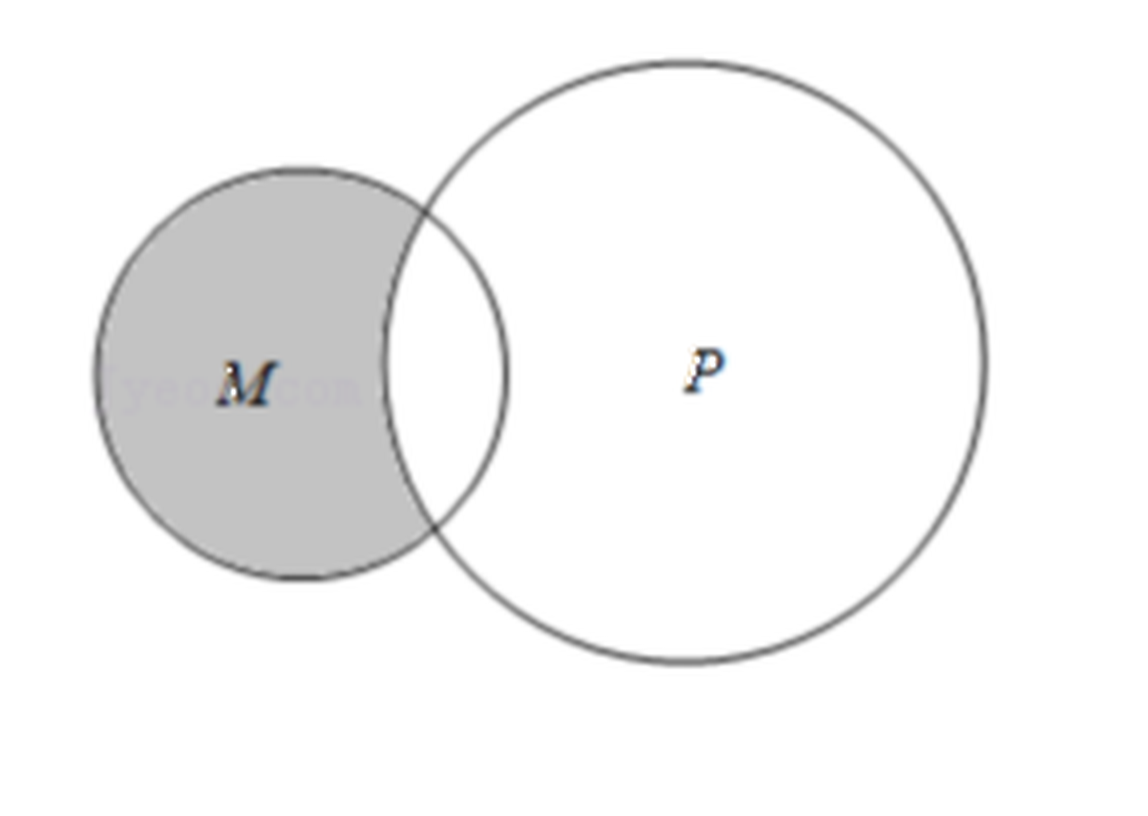
\includegraphics[width=0.36\textwidth]{figures/venn_M_shaded_P.png}
\end{center}

\step{阴影部分表示 $M-P$，所以 $M-(M-P)=M\cap P$. 故选 $B$.}
\solend

\fi

\item 设 $A_1$、$A_2$、$\cdots$、$A_7$ 均是含有 2 个元素的集合，且满足：

$A_i\cap A_{i+1}=\varnothing(i=1,2,3,4,5,6)$，$A_1\cap A_7=\varnothing$. 记 $B=A_1\cup A_2\cup\cdots\cup A_7$，则 $B$ 中元素个数的最小值是\mbox{（\quad）}

\keepwithprev
A. $4$\qquad B. $5$\qquad C. $6$\qquad D. $7$

\ans{$B$}

\ifanswer
\solbegin
\step{$A_1\cap A_7=\varnothing$，$A_i\cap A_{i+1}=\varnothing(i=1,2,3,4,5,6)$，}
\step{所以 $A_1$ 与 $A_2$ 的元素不同，则 $A_1\cup A_2$ 元素个数为 $4$，}
\step{若 $B$ 中元素个数的最小值是 $4$，则只能是 $A_3=A_1=A_5=A_7$，$A_4=A_2=A_6$，}
\step{与 $A_1\cap A_7=\varnothing$ 矛盾，}
\step{若 $A_3$ 从 $A_1$ 中选择 1 个元素，再加入一个新元素，}
\step{这样 $A_1\cup A_2\cup A_3$ 元素个数为 5 个，}
\step{这 5 个元素适当排列，得到 $A_4$、$A_5$、$A_6$、$A_7$，}
\step{例如 $A_1=\{1,2\},A_2=\{3,4\},A_3=\{1,5\}$，}
\step{取 $A_4=\{2,4\},A_5=\{3,5\},A_6=\{1,2\},A_7=\{3,5\}$，符合题意，}
\step{则 $B$ 中元素个数的最小值是 $2+2+1=5$，故选 $B$.}
\solend

\fi

\end{enumerate}

\bigsec{三、解答题}

\begin{enumerate}
\setcounter{enumi}{13}

\item 设 $A=\{x\mid x^2-ax+a^2-19=0\}$，$B=\{x\mid x^2-5x+6=0\}$，$C=\{x\mid x^2+2x-8=0\}$.

\begin{enumerate}[label=(\arabic*)]
\item 若 $A\cap B$ 非空，且 $A\cap C=\varnothing$，求 $a$ 的值；
\item $A\cap B=A\cap C\neq\varnothing$，求 $a$ 的值.
\end{enumerate}

\ifanswer
\solbegin
\stepm{(1)}{由题意，$C=\{-4,2\}$，}
\step{因为 $A\cap B$ 非空且 $A\cap C=\varnothing$，所以 $3\in A$，}
\step{即 $9-3a+a^2-19=0$，解得 $a=-2$ 或 $a=5$，}
\step{当 $a=-2$ 时，$A=\{3,-5\}$，满足题意；}
\step{当 $a=5$ 时，$A=\{2,3\}$，此时 $A\cap C=\{2\}$，不满足题意；}
\step{综上，$a=-2$；}
\stepm{(2)}{因为 $A\cap B=A\cap C\neq\varnothing$，所以 $2\in A$，}
\step{即 $4-2a+a^2-19=0$，解得 $a=-3$ 或 $a=5$，}
\step{当 $a=-3$ 时，$A=\{2,-5\}$，满足题意；}
\step{当 $a=5$ 时，$A=\{2,3\}$，不满足题意，}
\step{故 $a=-3$.}
\solend

\fi

\ansspace[6]

\item 已知 $A=\{x\mid x<-3\text{ 或 }x>1\}$.

\begin{enumerate}[label=(\arabic*)]
\item 若 $B=\{x\mid x<3m+1\text{ 或 }x>m+2\}$，$A\sub B$，求 $m$ 的取值范围.
\item 若 $B=\{x\mid m+2<x<3m+1\}$，$B\sub A$，求 $m$ 的取值范围.
\end{enumerate}

\ifanswer
\solbegin
\stepm{(1)}{当 $3m+1>m+2$，即 $m>\dfrac{1}{2}$ 时，$B=\R$，满足 $A\sub B$；}
\step{当 $3m+1\leqslant m+2$，即 $m\leqslant\dfrac{1}{2}$ 时，要使 $A\sub B$，}
\step{得 $\begin{cases}3m+1\geqslant-3\text{ ①}\\ m+2\leqslant 1\text{ ②}\end{cases}$，解得 $-\dfrac{4}{3}\leqslant m\leqslant-1$.}
\step{综上所述，$m$ 的取值范围为 $\left\{m\mid -\dfrac{4}{3}\leqslant m\leqslant-1\text{ 或 }m>\dfrac{1}{2}\right\}$；}
\stepm{(2)}{当 $B=\varnothing$ 时，则 $3m+1\leqslant m+2$，即 $m\leqslant\dfrac{1}{2}$ 时，满足 $B\sub A$；}
\step{当 $B\neq\varnothing$ 时，且 $B\sub A$，则 $\begin{cases}3m+1>m+2\\ 3m+1\leqslant-3\text{ 或 }m+2\geqslant 1\end{cases}$，所以 $m>\dfrac{1}{2}$.}
\step{综上所述，$m$ 的取值范围为 $\R$.}
\solend

\fi

\ansspace[6]

% 压轴题：其后已无内容，故作答区全用可丢弃胶水（\ansspace*），并在题目前先量一下版面。
\ansneed{7cm}

\item 已知集合 $A$ 为非空集合，定义

$S=\{x\mid x=a+b,a,b\in A\},T=\{x\mid x=|a-b|,a,b\in A\}$.

\begin{enumerate}[label=(\arabic*)]
\item 若集合 $A=\{1,3\}$，直接写出集合 $S$、$T$（无需写计算过程）；
\item 若集合 $A=\{x_1,x_2,x_3,x_4\}$，$x_1<x_2<x_3<x_4$，且 $T=A$，求证：$x_1+x_4=x_2+x_3$；
\item 若集合 $A=\{x\mid 0\leqslant x\leqslant 2021,x\in\N\}$，$S\cap T=\varnothing$. 记 $|A|$ 为集合 $A$ 中元素的个数，求 $|A|$ 的最大值.
\end{enumerate}

\ifanswer
\solbegin
\stepm{(1)}{$S=\{2,4,6\},T=\{0,2\}$；}
\stepm{(2)}{集合 $T$ 中最小的元素为 0，因为 $T=A$，且 $x_1<x_2<x_3<x_4$，所以 $x_1=0$，}
\step{所以集合 $T$ 中元素为 $x_2-x_1=x_2,x_3-x_1=x_3,x_4-x_1=x_4$，}
\step{以及 $x_3-x_2,x_4-x_2,x_4-x_3$ 均属于 $A$，}
% 注：本行原卷印「所以 $x_3$ 即 $x_4-x_2=x_3-x_1$」，「所以 $x_3$ 即 …」语义不完整，
%     疑有漏排（按本段结论应得 $x_4-x_2=x_3$），无法确证原意，本稿照抄原卷、未改。
\step{因为 $x_1=0<x_3-x_2<x_4-x_2<x_4$，所以 $x_3$ 即 $x_4-x_2=x_3-x_1$，}
\step{即 $x_1+x_4=x_2+x_3$；}
\stepm{(3)}{设 $A=\{a_1,a_2,a_3,\cdots,a_k\}$ 满足题意，其中 $a_1<a_2<\cdots<a_k$，}
\step{则 $2a_1<a_1+a_2<\cdots<a_1+a_k<a_2+a_k<a_3+a_k<\cdots<a_{k-1}+a_k<2a_k$，}
\step{所以 $|S\cup T|\leqslant 2k+1$，所以 $3k-1\leqslant 2a_k+1\leqslant 4043(k\in\N^*)$，}
\step{所以 $k\leqslant 1348$，}
\step{实际上当 $A=\{674,675,676,\cdots,2021\}$ 时满足题意，}
\step{证明如下：设 $A=\{m,m+1,m+2,\cdots,2021\},m\in\N$，}
\step{设 $S=\{2m,2m+1,2m+2,\cdots,4042\}$，$T=\{0,1,2,\cdots,2021-m\}$，}
\step{由题意得 $2021-m<2m$，即 $m>673\dfrac{2}{3}$，}
\step{故 $m$ 的最小值是 674，于是当 $m=674$，$A$ 中的元素最多，}
\step{即 $A=\{674,675,676,\cdots,2021\}$ 时满足题意，}
\step{综上所述，集合 $A$ 中元素的个数的最大值是 $1348$.}
\solend

\fi

\ansspace*[9]

\end{enumerate}

\bigsec{附加题}

\begin{enumerate}
\setcounter{enumi}{16}

\item 设 $A$ 是整数集的一个非空子集，对于 $k\in A$，如果 $k-1\notin A$ 且 $k+1\notin A$，那么 $k$ 是 $A$ 的一个“孤立元”。给定 $S=\{1,2,3,4,5,6,7,8\}$，由 $S$ 的 3 个元素构成的所有集合中，不含“孤立元”的集合共有 \blankline[2.4em] 个.

\ifanswer
\solbegin
\step{由题意得，“孤立元”即为在集合中无与之相邻的元素，}
\step{满足条件的集合有 $\{1,2,3\},\{2,3,4\},\{3,4,5\},\{4,5,6\},\{5,6,7\},\{6,7,8\}$，}
\step{共 6 个集合.}
\solend

\fi

\item 已知 $A\cap B=\varnothing$，$M=\{T\mid T\sub A\}$，$P=\{S\mid S\sub B\}$，则 $M\cap P=$ \blankline[4.4em].

\ans{$\{\varnothing\}$}

\item 已知集合 $A=\{x\mid x=m^2-n^2,m,n\in\Z\}$，写出所有满足集合 $A$ 的偶数 \blankline[4.4em].

\ans{$4n,n\in\Z$}

\item 对于给定的正整数 $n(n\geqslant 2)$ 若有限集合 $A=\{a_1,a_2,\cdots,a_n\}\sub M$，且满足

$a_1+a_2+\cdots+a_n=a_1\cdot a_2\cdots a_n$，则称 $A$ 为集合 $M$ 的 $n$ 元“调和子集”，则自然数集 $\N$ 的所有 3 元“调和子集”为 \blankline[3.6em].

\ans{$\{1,2,3\}$}

\end{enumerate}

\end{document}
"
%
% 原始材料是微信公众号图文（公众号「魔都数学加油站」），正文为 7 张 PNG 页（1080×1527）。
% 原文本身就是一份**讲评版**——题目下方直接印出【答案】或【解析】。试题文字、答案与解析
% 均照原卷录入，未改内容。卷面上的粉色斜水印「魔都数学加油站」属水印，未录入。
%
% 卷首标题：原卷印作「2026-2027 年七宝中学高一上抱孩子练习 9.8」——「抱孩子练习」四字
% 确系原卷所印（已放大 imgs_B/00.png 卷首核对），句末的「9.8」亦印在同一标题行内，
% 本稿一并照录，未改作「周末作业」；年份区间按全稿惯例排 en dash。
%
% 与原卷的排版差异（均已在 README「说明」中交代）：
%   ① 原文自**第 3 题**起（第 1、2 题未在该文中发布），故本稿题号亦自 3 起；
%   ② 原卷本就印有「一、填空题」「二、选择题」「三、解答题」三节标题，末节另印「附加题」，
%      本稿照原卷分节，只把标题改排成全稿统一的「大节标题」样式；
%   ③ 原卷填空、选择的答案直接印在题目下方，本稿统一改为试卷版隐去、答案版以【答案】或
%      【解析】给出（第 11 题原卷的答案是写在解析末句「故选 B」里的），使两版彻底分离；
%   ④ 原卷的集合符号 $R$、$Z$、$N$ 有正体与粗体两种写法（第 4 题的 $\mathbf{R}$、
%      第 16(3)、17、19、20 题的 $\mathbf{N}$、$\mathbf{Z}$ 为粗体，第 15 题解析的 $B=R$
%      为正体），本稿按全稿惯例统一写作 $\R$、$\Z$、$\N$；
%   ⑤ 原卷用**半角**括号（第 13 题「$\varnothing(i=1,2,3,4,5,6)$」、第 16(1)「(无需写计算过程)」、
%      第 16(2)「$A=\{x_1,x_2,x_3,x_4\}$」、第 20 题「$n(n\geqslant 2)$」），本稿按全稿惯例排全角；
%   ⑥ 原卷未印副标题，本稿按全稿惯例补出副标题「集合与常用逻辑用语」；
%   ⑦ 第 18、20 题的 $\subseteq$（带下划线，真包含写作 $\subset$ 与之形近）已逐处放大比对确认，
%      第 18 题的答案 $\{\varnothing\}$ 亦与 $\subseteq$ 口径相符（若为真包含则答案应为 $\varnothing$）。
%
% 原卷存疑两处（均已放大到能看清字形后核对，无法确证原意，本稿照抄原卷、未改）：
%   ① 第 10 题【解析】末句原卷印「所以 $1-k^2\neq 0$，即 $k\neq\pm 1$」——按此式，当 $k=1$
%      时两方程为同一直线、有无穷多解，$A\cap B\neq\varnothing$ 仍成立，故 $A\cap B\neq\varnothing$
%      当且仅当 $k\neq -1$；原卷结论与题设不合，疑为原卷笔误，但无法确证原意，本稿照抄原卷；
%   ② 第 16(2)【解析】原卷印「因为 $x_1=0<x_3-x_2<x_4-x_2<x_4$，所以 $x_3$ 即 $x_4-x_2=x_3-x_1$，」
%      ——「所以 $x_3$ 即 …」一句语义不完整，疑有漏排（按本段结论应得 $x_4-x_2=x_3$），
%      无法确证原意，本稿照抄原卷。

\documentclass[a4paper,11pt]{article}
\usepackage{common}

\begin{document}

\examtitlest[3]{2026--2027 年七宝中学高一上抱孩子练习 9.8}{集合与常用逻辑用语}

\bigsec{一、填空题}

\begin{enumerate}
\setcounter{enumi}{2}

\item 方程 $\sqrt{x+2}=-x$ 的解的集合为 \blankline[4.4em].

\ifanswer
\solbegin
\step{因为 $\sqrt{x+2}=-x$，所以 $\begin{cases}x\leqslant 0\\ x+2=x^2\end{cases}$，解得 $x=-1$，}
\step{所以方程 $\sqrt{x+2}=-x$ 的解的集合为 $\{-1\}$.}
\solend

\fi

\item 若 $A=\{x\mid a-4<x\leqslant a+4\}$，$B=\{x\mid x>5\text{ 或 }x<-1\}$，且 $A\cup B=\R$，则实数 $a$ 的取值范围是 \blankline[3.6em].

\ans{$[1,3)$}

\item 设集合 $A=\{x\mid x=2n+1,n\in\N\}$，$B=\{x\mid x=3n,n\in\N\}$，则 $A\cap B=$ \blankline[4.4em].

\ans{$\{x\mid x=6n+3,n\in\N\}$}

\item 已知集合 $A=\{1,2\}$，集合 $B=\{x\mid ax=6\}$，若 $A\cup B=A$，则 $a$ 的所有取值构成的集合为 \blankline[4.4em].

\ifanswer
\solbegin
\step{因为 $A\cup B=A$，所以 $B\sub A$，}
\step{当 $a=0$ 时，$B=\varnothing$，满足 $B\sub A$；}
\step{当 $a\neq 0$ 时，$B=\left\{\dfrac{6}{a}\right\}$，则 $\dfrac{6}{a}=1$ 或 $\dfrac{6}{a}=2$，解得 $a=6$ 或 $a=3$，}
\step{综上所述，$a$ 的所有取值构成的集合为 $\{0,3,6\}$.}
\solend

\fi

\item 设 $U=\{2,4,a^2-a+1\}$，$A=\{2,|a+1|\}$，$\overline{A}=\{7\}$，则 $a=$ \blankline[2.4em].

\ans{$3$}

\item 已知集合 $A=\{x\mid x^2-px-q=0\}$，$B=\{x\mid x^2+qx-p=0\}$，且 $A\cap B=\{1\}$，则 $A\cup B=$ \blankline[4.4em].

\ans{$\{0,-1,1\}$}

\item 定义集合运算：$A\odot B=\{z\mid z=xy(x+y),x\in A,y\in B\}$，若 $A=\{1,2\},B=\{3,4\}$，则 $A\odot B$ 的所有元素之和是 \blankline[3.6em].

\ans{$110$}

\item 已知集合 $A=\{(x,y)\mid kx+y=k+1\}$，$B=\{(x,y)\mid x+ky=2k\}$，其中 $k$ 为实数，$A\cap B\neq\varnothing$，则 $k$ 的取值范围是 \blankline[4.4em].

\ifanswer
\solbegin
\step{因为 $A\cap B\neq\varnothing$，所以方程组 $\begin{cases}kx+y=k+1\\ x+ky=2k\end{cases}$ 有解，消 $y$ 得 $(1-k^2)x=k-k^2$，}
% 注：末句原卷印「所以 $1-k^2\neq 0$，即 $k\neq\pm 1$」。按此式，$k=1$ 时两方程为同一直线、
%     有无穷多解，$A\cap B\neq\varnothing$ 仍成立，故结论应为 $k\neq -1$。疑为原卷笔误，
%     但无法确证原意，本稿照抄原卷、未改（详见文件头「原卷存疑」①）。
\step{所以 $1-k^2\neq 0$，即 $k\neq\pm 1$.}
\solend

\fi

\end{enumerate}

\bigsec{二、选择题}

\begin{enumerate}
\setcounter{enumi}{10}

\item 给出关系式：①$0\in\varnothing$；②$\varnothing=\{0\}$；③$\{a,b\}=\{b,a\}$；④$\{y\mid y=x^2-2\}=\{(x,y)\mid y=x^2-2\}$，其中正确的关系式的个数是\mbox{（\quad）}

\keepwithprev
A. $0$\qquad B. $1$\qquad C. $2$\qquad D. $3$

\ans{$B$}

\ifanswer
\solbegin
\step{在①中，$\varnothing$ 表示空集，$0\notin\varnothing$，故①错误；在②中，$\varnothing\sub\{0\}$，故②错误；}
\step{在③中，$\{a,b\}=\{b,a\}$，故③正确；}
\step{在④中，因为，$\{y\mid y=x^2-2\}$ 和 $\{(x,y)\mid y=x^2-2\}$ 的代表元素不同，}
\step{所以 $\{y\mid y=x^2-2\}\neq\{(x,y)\mid y=x^2-2\}$，故④错误.}
\step{故正确的是③，故选 $B$.}
\solend

\fi

\item 设集合 $M$、$P\neq\varnothing$，定义集合 $M-P=\{x\mid x\in M,x\notin P\}$，则集合 $M-(M-P)$ 是\mbox{（\quad）}

\keepwithprev
A. $P$\qquad B. $M$\qquad C. $M\cup P$\qquad D. $M\cap P$

\ans{$B$}

\ifanswer
\solbegin
\step{$M-(M-P)=\{x\mid x\in M,\text{ 且 }x\notin(M-P)\}$，}
\step{用 venn 图表示集合 $M$、$P$ 的关系如图：}

\begin{center}
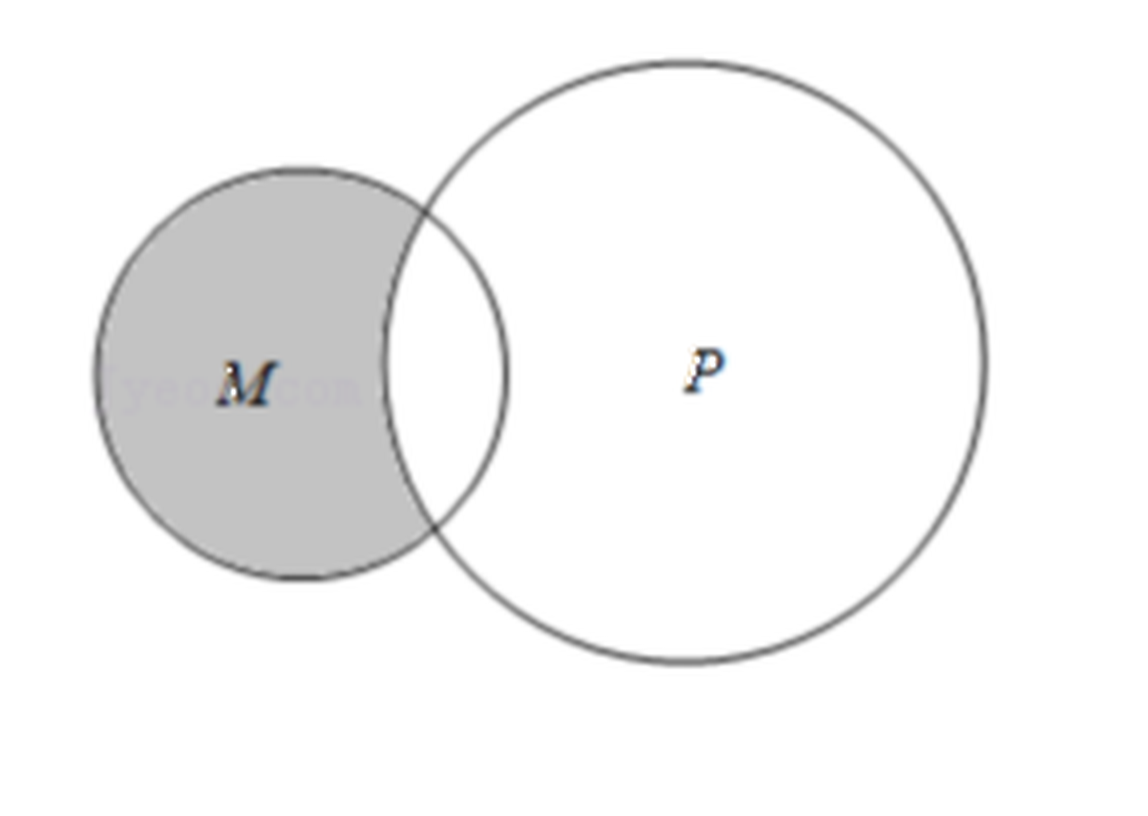
\includegraphics[width=0.36\textwidth]{figures/venn_M_shaded_P.png}
\end{center}

\step{阴影部分表示 $M-P$，所以 $M-(M-P)=M\cap P$. 故选 $B$.}
\solend

\fi

\item 设 $A_1$、$A_2$、$\cdots$、$A_7$ 均是含有 2 个元素的集合，且满足：

$A_i\cap A_{i+1}=\varnothing(i=1,2,3,4,5,6)$，$A_1\cap A_7=\varnothing$. 记 $B=A_1\cup A_2\cup\cdots\cup A_7$，则 $B$ 中元素个数的最小值是\mbox{（\quad）}

\keepwithprev
A. $4$\qquad B. $5$\qquad C. $6$\qquad D. $7$

\ans{$B$}

\ifanswer
\solbegin
\step{$A_1\cap A_7=\varnothing$，$A_i\cap A_{i+1}=\varnothing(i=1,2,3,4,5,6)$，}
\step{所以 $A_1$ 与 $A_2$ 的元素不同，则 $A_1\cup A_2$ 元素个数为 $4$，}
\step{若 $B$ 中元素个数的最小值是 $4$，则只能是 $A_3=A_1=A_5=A_7$，$A_4=A_2=A_6$，}
\step{与 $A_1\cap A_7=\varnothing$ 矛盾，}
\step{若 $A_3$ 从 $A_1$ 中选择 1 个元素，再加入一个新元素，}
\step{这样 $A_1\cup A_2\cup A_3$ 元素个数为 5 个，}
\step{这 5 个元素适当排列，得到 $A_4$、$A_5$、$A_6$、$A_7$，}
\step{例如 $A_1=\{1,2\},A_2=\{3,4\},A_3=\{1,5\}$，}
\step{取 $A_4=\{2,4\},A_5=\{3,5\},A_6=\{1,2\},A_7=\{3,5\}$，符合题意，}
\step{则 $B$ 中元素个数的最小值是 $2+2+1=5$，故选 $B$.}
\solend

\fi

\end{enumerate}

\bigsec{三、解答题}

\begin{enumerate}
\setcounter{enumi}{13}

\item 设 $A=\{x\mid x^2-ax+a^2-19=0\}$，$B=\{x\mid x^2-5x+6=0\}$，$C=\{x\mid x^2+2x-8=0\}$.

\begin{enumerate}[label=(\arabic*)]
\item 若 $A\cap B$ 非空，且 $A\cap C=\varnothing$，求 $a$ 的值；
\item $A\cap B=A\cap C\neq\varnothing$，求 $a$ 的值.
\end{enumerate}

\ifanswer
\solbegin
\stepm{(1)}{由题意，$C=\{-4,2\}$，}
\step{因为 $A\cap B$ 非空且 $A\cap C=\varnothing$，所以 $3\in A$，}
\step{即 $9-3a+a^2-19=0$，解得 $a=-2$ 或 $a=5$，}
\step{当 $a=-2$ 时，$A=\{3,-5\}$，满足题意；}
\step{当 $a=5$ 时，$A=\{2,3\}$，此时 $A\cap C=\{2\}$，不满足题意；}
\step{综上，$a=-2$；}
\stepm{(2)}{因为 $A\cap B=A\cap C\neq\varnothing$，所以 $2\in A$，}
\step{即 $4-2a+a^2-19=0$，解得 $a=-3$ 或 $a=5$，}
\step{当 $a=-3$ 时，$A=\{2,-5\}$，满足题意；}
\step{当 $a=5$ 时，$A=\{2,3\}$，不满足题意，}
\step{故 $a=-3$.}
\solend

\fi

\ansspace[6]

\item 已知 $A=\{x\mid x<-3\text{ 或 }x>1\}$.

\begin{enumerate}[label=(\arabic*)]
\item 若 $B=\{x\mid x<3m+1\text{ 或 }x>m+2\}$，$A\sub B$，求 $m$ 的取值范围.
\item 若 $B=\{x\mid m+2<x<3m+1\}$，$B\sub A$，求 $m$ 的取值范围.
\end{enumerate}

\ifanswer
\solbegin
\stepm{(1)}{当 $3m+1>m+2$，即 $m>\dfrac{1}{2}$ 时，$B=\R$，满足 $A\sub B$；}
\step{当 $3m+1\leqslant m+2$，即 $m\leqslant\dfrac{1}{2}$ 时，要使 $A\sub B$，}
\step{得 $\begin{cases}3m+1\geqslant-3\text{ ①}\\ m+2\leqslant 1\text{ ②}\end{cases}$，解得 $-\dfrac{4}{3}\leqslant m\leqslant-1$.}
\step{综上所述，$m$ 的取值范围为 $\left\{m\mid -\dfrac{4}{3}\leqslant m\leqslant-1\text{ 或 }m>\dfrac{1}{2}\right\}$；}
\stepm{(2)}{当 $B=\varnothing$ 时，则 $3m+1\leqslant m+2$，即 $m\leqslant\dfrac{1}{2}$ 时，满足 $B\sub A$；}
\step{当 $B\neq\varnothing$ 时，且 $B\sub A$，则 $\begin{cases}3m+1>m+2\\ 3m+1\leqslant-3\text{ 或 }m+2\geqslant 1\end{cases}$，所以 $m>\dfrac{1}{2}$.}
\step{综上所述，$m$ 的取值范围为 $\R$.}
\solend

\fi

\ansspace[6]

% 压轴题：其后已无内容，故作答区全用可丢弃胶水（\ansspace*），并在题目前先量一下版面。
\ansneed{7cm}

\item 已知集合 $A$ 为非空集合，定义

$S=\{x\mid x=a+b,a,b\in A\},T=\{x\mid x=|a-b|,a,b\in A\}$.

\begin{enumerate}[label=(\arabic*)]
\item 若集合 $A=\{1,3\}$，直接写出集合 $S$、$T$（无需写计算过程）；
\item 若集合 $A=\{x_1,x_2,x_3,x_4\}$，$x_1<x_2<x_3<x_4$，且 $T=A$，求证：$x_1+x_4=x_2+x_3$；
\item 若集合 $A=\{x\mid 0\leqslant x\leqslant 2021,x\in\N\}$，$S\cap T=\varnothing$. 记 $|A|$ 为集合 $A$ 中元素的个数，求 $|A|$ 的最大值.
\end{enumerate}

\ifanswer
\solbegin
\stepm{(1)}{$S=\{2,4,6\},T=\{0,2\}$；}
\stepm{(2)}{集合 $T$ 中最小的元素为 0，因为 $T=A$，且 $x_1<x_2<x_3<x_4$，所以 $x_1=0$，}
\step{所以集合 $T$ 中元素为 $x_2-x_1=x_2,x_3-x_1=x_3,x_4-x_1=x_4$，}
\step{以及 $x_3-x_2,x_4-x_2,x_4-x_3$ 均属于 $A$，}
% 注：本行原卷印「所以 $x_3$ 即 $x_4-x_2=x_3-x_1$」，「所以 $x_3$ 即 …」语义不完整，
%     疑有漏排（按本段结论应得 $x_4-x_2=x_3$），无法确证原意，本稿照抄原卷、未改。
\step{因为 $x_1=0<x_3-x_2<x_4-x_2<x_4$，所以 $x_3$ 即 $x_4-x_2=x_3-x_1$，}
\step{即 $x_1+x_4=x_2+x_3$；}
\stepm{(3)}{设 $A=\{a_1,a_2,a_3,\cdots,a_k\}$ 满足题意，其中 $a_1<a_2<\cdots<a_k$，}
\step{则 $2a_1<a_1+a_2<\cdots<a_1+a_k<a_2+a_k<a_3+a_k<\cdots<a_{k-1}+a_k<2a_k$，}
\step{所以 $|S\cup T|\leqslant 2k+1$，所以 $3k-1\leqslant 2a_k+1\leqslant 4043(k\in\N^*)$，}
\step{所以 $k\leqslant 1348$，}
\step{实际上当 $A=\{674,675,676,\cdots,2021\}$ 时满足题意，}
\step{证明如下：设 $A=\{m,m+1,m+2,\cdots,2021\},m\in\N$，}
\step{设 $S=\{2m,2m+1,2m+2,\cdots,4042\}$，$T=\{0,1,2,\cdots,2021-m\}$，}
\step{由题意得 $2021-m<2m$，即 $m>673\dfrac{2}{3}$，}
\step{故 $m$ 的最小值是 674，于是当 $m=674$，$A$ 中的元素最多，}
\step{即 $A=\{674,675,676,\cdots,2021\}$ 时满足题意，}
\step{综上所述，集合 $A$ 中元素的个数的最大值是 $1348$.}
\solend

\fi

\ansspace*[9]

\end{enumerate}

\bigsec{附加题}

\begin{enumerate}
\setcounter{enumi}{16}

\item 设 $A$ 是整数集的一个非空子集，对于 $k\in A$，如果 $k-1\notin A$ 且 $k+1\notin A$，那么 $k$ 是 $A$ 的一个“孤立元”。给定 $S=\{1,2,3,4,5,6,7,8\}$，由 $S$ 的 3 个元素构成的所有集合中，不含“孤立元”的集合共有 \blankline[2.4em] 个.

\ifanswer
\solbegin
\step{由题意得，“孤立元”即为在集合中无与之相邻的元素，}
\step{满足条件的集合有 $\{1,2,3\},\{2,3,4\},\{3,4,5\},\{4,5,6\},\{5,6,7\},\{6,7,8\}$，}
\step{共 6 个集合.}
\solend

\fi

\item 已知 $A\cap B=\varnothing$，$M=\{T\mid T\sub A\}$，$P=\{S\mid S\sub B\}$，则 $M\cap P=$ \blankline[4.4em].

\ans{$\{\varnothing\}$}

\item 已知集合 $A=\{x\mid x=m^2-n^2,m,n\in\Z\}$，写出所有满足集合 $A$ 的偶数 \blankline[4.4em].

\ans{$4n,n\in\Z$}

\item 对于给定的正整数 $n(n\geqslant 2)$ 若有限集合 $A=\{a_1,a_2,\cdots,a_n\}\sub M$，且满足

$a_1+a_2+\cdots+a_n=a_1\cdot a_2\cdots a_n$，则称 $A$ 为集合 $M$ 的 $n$ 元“调和子集”，则自然数集 $\N$ 的所有 3 元“调和子集”为 \blankline[3.6em].

\ans{$\{1,2,3\}$}

\end{enumerate}

\end{document}
